\documentclass{kti}

% ----------------------------------------
% Metadata
% ----------------------------------------
\faculty{Fakultas Pendidikan Matematika dan Ilmu Pengetahuan Alam}
\department{Departemen Pendidikan Ilmu Komputer}
\program{Program Studi Ilmu Komputer}
\title{Pengenalan Emosi Manusia Menggunakan \textit{Log-Gabor Convolutional Networks} Melalui Pendekatan \textit{Facial Region Segmentation}}
\titleen{Human Emotion Recognition Using \textit{Log-Gabor Convolutional Networks} Through \textit{Facial Region Segmentation} Approach}
\author{Naufan Rusyda Faikar}
\email{nrfaikar@student.upi.edu}
\studentid{1607645}
\monthsubmit{Agustus}
\yearsubmit{2020}
\firstsupervisorname{Prof. Dr. H. Wawan Setiawan, M.Kom}
\firstsupervisorid{196601011991031005}
\secondsupervisorname{Yaya Wihardi, S.Kom., M.Kom.}
\secondsupervisorid{198903252015041001}
\departmentheadname{Dr. Lala Septem Riza, M.T.}
\departmentheadid{197811262008121001}

% TODO: cek kembali secara menyeluruh
\hyphenation{meng-gu-na-kan seg-men-ta-tion me-ngu-kur me-nye-sat-kan me-nge-na-li pe-nge-na-lan pe-ne-ra-pan ek-strak-si di-man-fa-at-kan eks-pre-si re-le-van ha-ra-pan men-cer-min-kan meng-hu-bung-kan key-board di-u-sul-kan di-la-ku-kan di-gu-na-kan me-nge-na-kan di-sip-lin neu-ron pe-la-ti-han di-ru-mus-kan craw-ling en-hance-ment akan ber-da-sar-kan me-nga-dop-si di-sim-pan me-ne-rap-kan me-ning-kat-kan ke-se-lu-ru-han me-lan-jut-kan di-ten-tu-kan di-per-li-hat-kan ke-sa-la-han dis-gust weighted di-per-lu-kan neu-tral men-ja-jar-kan ka-nan net-work en-sem-ble}

\begin{document}

\frontmatter
% ----------------------------------------
% Halaman judul
% ----------------------------------------
\cover

% ----------------------------------------
% Halaman hak cipta
% ----------------------------------------
\copyright

% ----------------------------------------
% Halaman pengesahan
% ----------------------------------------
\approval

% ----------------------------------------
% Halaman pernyataan keaslian dan bebas
% plagiarisme
% ----------------------------------------
\statementcontent{Saya menyatakan bahwa skripsi berjudul ``Pengenalan Emosi Manusia Menggunakan \textit{Log-Gabor Convolutional Networks} Melalui Pendekatan \textit{Facial Region Segmentation}'' ini adalah benar karya saya sendiri. Dan saya tidak melakukan tindakan plagiat yang menyalahi etika dalam karya tulis ilmiah. Apabila saya terbukti bersalah, maka saya bersedia untuk memperbaiki diri, meminta maaf kepada pihak yang bersangkutan dan menanggung setiap sanksi yang berlaku.}
\statement

% ----------------------------------------
% Halaman ucapan terima kasih/persembahan
% ----------------------------------------
\acknowledgmentcontent{Untuk ibu, bapak\\dan adik-adikku tercinta.}
\acknowledgment

% ----------------------------------------
% Kata pengantar
% ----------------------------------------
\prefacecontent{Segala puji bagi Allah \textit{Subh\=anahu wa Ta’\=ala}, yang dengan nikmat-Nya maka sempurnalah segala kebaikan. Tiada daya dan upaya kecuali hanya dari-Nya. Hanya dengan memohon pertolongan-Nya, penulis dapat menyelesaikan skripsi berjudul ``Pengenalan Emosi Manusia dengan \textit{Log-Gabor Convolutional Networks} Melalui Pendekatan \textit{Facial Region Segmentation}'' ini tepat waktu. Skripsi ini disusun dalam rangka memenuhi sebagian syarat memperoleh gelar Sarjana S-1 Jurusan Ilmu Komputer di Universitas Pendidikan Indonesia.

Pada kenyataannya, skripsi ini bukan merupakan kredit tersendiri bagi penulis. Melainkan merupakan upaya murni kolaboratif dengan berbagai pihak selama penulis belajar di bangku perkuliahan. Setelah memulai dengan mengucapkan syukur kepada Allah \textit{Subh\=anahu wa Ta’\=ala} di atas segalanya, penulis ingin mengucapkan terima kasih yang tulus kepada kedua pembimbing skripsi ini, bapak Yaya Wihardi dan bapak Wawan Setiawan, karena telah bersedia dengan sepenuh hati membimbing penulis dalam menyelesaikan skripsi ini.

Sejak diberikan kesempatan oleh bapak Yaya untuk bergabung bersama beliau, bapak Wawan, ibu Enjun Junaeti dan keempat anggota lain dalam riset \textit{smart classroom}, penulis merasa lebih beruntung dari kebanyakan teman-teman lain. Selama melakukan riset bersama-sama, penulis telah banyak belajar dari berbagai tahap yang telah dilalui.

Penulis ingin mengucapkan terima kasih sebanyak-banyaknya kepada bapak Yaya sebagai mentor terbaik. Selama melakukan bimbingan, beliau telah memberikan sebuah advis kepada penulis bahwa skripsi yang bagus adalah yang selesai. Ketika skripsi itu harus tertunda penyelesaiannya karena ingin serba perfek, maka akan banyak peluang yang mungkin terlewatkan. Terus terang, penulis sangat menyukai bagaimana beliau mengumpulkan setiap mahasiswanya di ruangan yang sama untuk melakukan bimbingan pekanan. Dengan begitu, penulis telah mendapatkan berbagai masukan dan pandangan yang berbeda dari beliau sendiri dan teman-teman saat itu. Selama mengikuti kelas, penulis telah banyak belajar dari beliau khususnya mengenai \textit{computer vision} dan \textit{image processing}. Bagi penulis, beliau termasuk salah satu dosen yang paling cakap dalam mengajar. Sebagai salah satu anggota laboratorium Kecerdasan Buatan dan Robotika, beliau telah meneladani penulis untuk memiliki loyalitas dan kedisplinan yang tinggi.

Juga terima kasih kepada bapak Wawan yang telah mempercayai penulis sebagai salah satu anggota riset \textit{smart classroom} yang beliau ketuai. Tanpa dukungan yang besar dari beliau, penulis tidak akan memiliki kesempatan untuk dapat bermalam di kampus dan menuntaskan proyek akhir robotika.

Penulis merasa sangat bersyukur telah diberikan kesempatan dan kepercayaan dalam mengajar sebagai asisten dari ibu Rani Megasari di kelas Basis Data, bapak Yudi Wibisono di kelas Sistem Basis Data, bapak Herbert Siregar di kelas Pemrograman Visual dan bapak Eddy Prasetyo Nugroho di kelas Rekayasa Perangkat Lunak. Terima kasih juga kepada teman-teman yang telah menjadi partner mengajar yang kompeten. Dengan mengajar, penulis tidak hanya mendapatkan pengetahuan yang lebih luas dan mendalam mengenai bahan ajar yang disampaikan, namun juga mendapatkan keluasan untuk meningkatkan kemampuan mengajar dan berbicara di depan kelas. Penulis menjadi mengerti bahwa menempatkan diri bukan sebagai pengajar, akan tetapi sebagai partner bagi para studen, penting dilakukan dalam mengajar di kelas. Hubungan emosional yang baik sedikit banyak mempengaruhi motivasi mereka dalam mengikuti kelas.

Penulis merasa sangat beruntung telah memiliki dosen-dosen yang istimewa. Sangat menyenangkan mendengarkan mereka saling menceritakan kisah inspiratif satu sama lain. Selain yang sudah disebutkan di atas, penulis ingin berterima kasih lebih khusus kepada ibu Rosa Ariani Sukamto yang telah mengajarkan penulis untuk tidak perlu menjadi orang lain, untuk selalu jujur dalam berlaku dan untuk selalu berjuang juga tidak malu dalam belajar. Juga kepada bapak Yudi yang telah mengajarkan penulis untuk tidak takut berbuat kesalahan dalam belajar dan untuk tidak berhenti belajar sebelum mampu menghasilkan buah karya. Juga kepada bapak Herbert Siregar yang telah mengajarkan penulis untuk selalu belajar memahami sesuatu secara mendasar dan untuk selalu memiliki etos juga etika dalam bekerja. Juga kepada bapak Eddy yang telah mengajarkan penulis untuk selalu menilai sesuatu secara adil juga lugas. Juga kepada ibu Enjun yang telah mengajarkan penulis untuk selalu mengutamakan disiplin dalam berlaku dan untuk selalu menghargai usaha orang lain. Juga kepada dosen-dosen lain yang tidak dapat disebutkan satu per satu. Namun, satu hal yang dapat dipastikan bahwa penulis telah belajar banyak sekali makna dari mereka semua. Jika diperbolehkan, penulis ingin selalu dapat duduk setidaknya satu kali lagi di hadapan mereka untuk mendengarkan dan mencatat beberapa pelajaran terakhir.

Tidak lupa, penulis juga ingin mengucapkan terima kasih kepada teman-teman yang telah memberikan warna dan menyulap setiap kebersamaan kami dalam belajar di kelas menjadi sangat menyenangkan dan tidak akan pernah tergantikan. Yang telah membuat kenangan dalam ruang-ruang kelas tidak akan pernah sama jika tanpa mereka. Secara istimewa, penulis ingin berterima kasih sebanyak-banyaknya kepada Muhammad Faris Muzakki dan Yahya Firdaus yang telah menjadi partner dalam banyak pekerjaan. Juga kepada Ammar Ashshiddiqi, Reyhan Fikri Dzikriansyah, Teguh Arianto,, Adnan Khairi As., Asep Saepul Ahmad, I. G. N. Agung A. A. W., dan Genta Satria A. P. sebagai teman-teman terdekat penulis dalam menjalani kehidupan di kampus. Juga kepada kakak-kakak tingkat yang telah bersedia menjawab dan memandu penulis dengan begitu tulus dan tanpa pamrih dalam belajar.

Setiap momen yang penulis habiskan bersama teman-teman seperjuangan adalah menyenangkan dan tidak akan tergantikan. Di sisi lain, setiap momen duduk mencatat dan mengacungkan tangan bertanya mengenai setiap pelajaran yang disampaikan oleh dosen-dosen yang berdedikasi juga tidak akan terlupakan. Bersama dengan mereka semua, kami telah saling berbagi banyak pengetahuan dan cerita.

Tanpa henti-hentinya, penulis juga bersyukur telah diberikan keluarga yang selalu menjadi orang-orang yang paling pertama dan paling setia dalam mendukung setiap keputusan penulis. Mereka adalah abi Ahmad Djunaedi Sastradinata, umi Desy Rosika Natalia, Ahmad Faaiz Al-Auza'i, Salma Kaisan Syauqi dan Kaisa Rifqa Ghassani. Tanpa doa dan dukungan dari mereka semua, penulis tidak akan mampu berdiri dan melangkah di atas kaki sendiri menuju perjalanan yang penuh dengan kebahagiaan.

Terakhir, penulis ingin berterima kasih kepada bapak Lala Septem Riza selaku Ketua Departemen Pendidikan Ilmu Komputer Universitas Pendidikan Indonesia, ibu Rani selaku Ketua Program Studi Ilmu Komputer Universitas Pendidikan Indonesia serta semua dosen penguji proposal juga laporan akhir skripsi ini.

Demikian pengantar ini dibuat dengan sungguh-sungguh. Penulis berharap bahwa pekerjaan ini dapat bermanfaat bagi penulis sendiri dan seluruh pembaca budiman. \textit{At last but not least}, penulis menyatakan secara terbuka untuk menerima segala masukan dalam menyempurnakan skripsi ini.}
\preface

% ----------------------------------------
% Abstrak
% ----------------------------------------
\abstractcontent{Pengenalan emosi manusia secara otomatis dapat bermanfaat pada sektor-sektor terkait komputasi afektif. Penelitian ini merupakan penelitian pertama yang mengadopsi teknik \textit{facial region segmentation} (FRS) pada arsitektur \textit{Log-Gabor Convolutional Networks} (Log-GCNs) dalam membangun model menggunakan set data gambar wajah nonfrontal, FER-2013. Dengan menggunakan deteksi \textit{facial landmark}, daerah fitur wajah tertentu dapat disegmentasi menjadi dua-tiga bagian. Setiap bagian dapat dilatih baik secara individu maupun bersamaan menggunakan teknik \textit{network ensemble}, di mana sejumlah arsitektur GCN yang identik tergabung di dalamnya. Hasil eksperimen membuktikan bahwa Log-GCN dengan FRS berhasil mengungguli \emph{baseline} dengan augmentasi data melalui peningkatan akurasi sebesar 6,07\%.}
\abstractkeywords{Rekognisi emosi; rekognisi ekspresi wajah; FER; segmentasi daerah wajah; \textit{deep convolutional neural network}; jaringan ansambel.}

\abstractencontent{Automatic recognition of human emotions can be useful in sectors related to affective computing. We believe that it is the first study to adopt facial region segmentation (FRS) techniques on the Log-Gabor Convolutional Networks (Log-GCNs) architecture in order to build a model that using the non-frontal face dataset images, FER-2013. By using facial landmarks detection, certain facial feature areas can be segmented into two-three parts. Each region can be trained either individually or together using network ensemble techniques, where a number of identical GCN architectures are combined. The experimental results prove that Log-GCN with FRS successfully outperformed the baseline with data augmentation through an increase in accuracy of 6.07\%.}
\abstractenkeywords{Emotion recognition; facial expression recognition; FER; facial region segmentation; deep convolutional neural network; network ensemble.}
\abstract

% ----------------------------------------
% Daftar isi
% ----------------------------------------
\addcontentsline{toc}{chapter}{DAFTAR ISI}
\tableofcontents

% ----------------------------------------
% Daftar tabel
% ----------------------------------------
\listoftables
\addcontentsline{toc}{chapter}{DAFTAR TABEL}

% ----------------------------------------
% Daftar gambar
% ----------------------------------------
\listoffigures
\addcontentsline{toc}{chapter}{DAFTAR GAMBAR}

% ----------------------------------------
% Daftar lampiran
% ----------------------------------------
% [TODO]

\newpage
\mainmatter
% ----------------------------------------
% Isi
% ----------------------------------------
\chapter{Pendahuluan}
Pada bab ini disajikan latar belakang penelitian pengenalan emosi manusia meliputi jawaban atas pertanyaan-pertanyaan mengapa domain penelitian ini menarik dan penting untuk dilakukan, bagaimana peluang aplikasi dari hasil penelitian ini, bagaimana alur kerja pemodelan pengenalan emosi manusia, bagaimana pencapaian terkini dari penelitian terkait, bagaimana pendekatan yang diusulkan serta peluang keberhasilannya. Kemudian dipaparkan mengenai identifikasi masalah, rumusan masalah, tujuan penelitian, batasan penelitian dan manfaat penelitian yang relevan. Diakhiri dengan penjelasan struktur organisasi penulisan skripsi ini dari Bab I hingga Bab V dan bagian-bagian pelengkap lainnya.

\section{Latar Belakang}
Pengenalan emosi manusia sangat banyak manfaatnya, terutama pada sektor-sektor terkait \gls{komputasiafektif}\footnote{Komputasi afektif adalah studi multidisipliner pada pengembangan sistem yang mampu mengenali, memahami dan menghasilkan emosi manusia.}. Pada periklanan umpamanya, pengenalan emosi dapat diterapkan berdasarkan hubungan berbanding lurus antara kualitas respons emosional masyarakat terhadap iklan dengan peningkatan penjualan \shortcite{sujata2018facial}. Pada rekayasa perangkat lunak, pengenalan emosi dapat dimanfaatkan, baik untuk menilai efisiensi kerja dan kualitas kode tiap-tiap karyawan maupun untuk mengukur kepuasan pelanggan guna menggantikan penggunaan kuisoner yang menyesatkan \shortcite{kolakowska2013emotion,kolakowska2014emotion}. \shortciteA{beccue2018exsum} mengidentifikasi setidaknya terdapat tujuh peluang pasar dalam penggunaan teknologi ini yang tetap relevan hingga 2025 mendatang, yaitu untuk diterapkan pada layanan pelanggan, penelitian produk/pasar, pengalaman pelanggan, perawatan kesehatan, pendidikan, otomotif, dan gim.

Pengenalan emosi memberikan kemampuan tiruan kepada sistem komputer untuk dapat menafsirkan bermacam-macam emosi manusia. Untuk mencapai tujuan tersebut, berbagai pendekatan komunikasi telah dilakukan, baik itu \gls{komunikasiverbal} maupun nonverbal\footnote{Komunikasi verbal melibatkan kata-kata, baik lisan maupun tulisan. Sebaliknya, komunikasi nonverbal melibatkan perilaku fisik (bahasa tubuh), meliputi ekspresi wajah, postur tubuh dan isyarat.} \shortcite{garcia2017emotion}. Sejauh ini, pengenalan emosi melalui ekspresi wajah diklaim paling akurat. Sebab ekspresi wajah, dalam kasus terbanyak, memiliki kontribusi terbesar dalam komunikasi \shortcite{mehrabian1967decoding,mehrabian1967inference,lapakko2007communication}. Disertai asumsi bahwa sejumlah ekspresi wajah manusia bersifat universal\footnote{Set emosi yang terdiri dari enam kelas emosi (\textit{six basic emotions}), yang dianggap universal oleh \shortciteA{ekman1970universal}, meliputi \textit{angry}, \textit{disgust}, \textit{fear}, \textit{happy}, \textit{sad}, dan \textit{surprise}.}, pengenalan emosi sangat mungkin dilakukan melalui proses analisis ekspresi wajah \shortcite{ekman1970universal}.

Pengenalan ekspresi wajah termasuk kajian multidisipliner \shortcite{mandal2014understanding}, yang tidak hanya bersifat teoretis ---tentang bagaimana ekspresi wajah menyatakan emosi manusia---, melainkan juga bersifat teknis ---tentang bagaimana komputer dapat meniru kemampuan emosi manusia--- \shortcite{ekman1993facial,gendron2014perceptions,jack2012facial}. Atas kemajuan teknologi yang kian canggih, perbalahan teoretis tidak lagi kentara. Meskipun manusia belum mampu sepenuhnya untuk menjelaskan setiap aspek di dalamnya, akan tetapi \textit{machine learning} \shortcite{hebb1949organization} telah terbukti berhasil menyelesaikan masalah-masalah terkait rekognisi secara akurat. Tidak hanya dapat mengenali emosi manusia, teknologi rekognisi saat ini telah mampu mengenali emosi kucing \shortcite{evangelista2019facial} dan anjing \shortcite{amici2019ability}. Sehingga penggunaan \textit{machine learning} pada pengenalan ekspresi wajah mengetren dewasa ini.

Hingga saat ini, keberhasilan teknologi rekognisi sangat bergantung kepada kuantitas dan kualitas set data yang digunakan. Set data ekspresi wajah yang sangat bervariasi, meliputi variasi karakteristik subjek ---seperti ras, etnis, jenis kelamin dan usia--- dan potret ---seperti kualitas gambar; rotasi, sudut dan jarak pengambilan--- merupakan sebuah tantangan besar bagi penelitian pengenalan ekspresi wajah. Untuk menyeragamkan distribusi probabilitas set data ekspresi wajah, pengambilan set data sering kali dilakukan pada kondisi lingkungan yang sudah diatur sedemikian rupa. Pengambilan dengan cara demikian mengacu kepada pemotretan ekspresi wajah menggunakan sisi depan wajah untuk menghasilkan set data wajah frontal \shortcite{lucey2010extended}. Melalui cara ini, penelitian mutakhir pada pengenalan ekspresi wajah frontal mampu mencapai akurasi sempurna pada data wajah frontal \shortcite{zhou2019facial}.-

Terlepas dari banyaknya usaha dan mahalnya biaya yang harus diberikan untuk mengakuisisi set data wajah frontal, penggunaan set data frontal memiliki beberapa kerugian yang berarti. Dalam banyak skenario praktis, model rekognisi yang dilatih menggunakan set data wajah frontal menjadi tidak relevan untuk penerapan dalam kondisi liar. Sebab data input aplikasi diperoleh di bawah pengaturan lingkungan dan peralatan yang berbeda. Pada sebagian besar kasus, pengambilan potret wajah subjek tidak dilakukan dalam posisi yang sejajar dengan sensor kamera. Contohnya pada aplikasi pendeteksi emosi pengemudi kendaraan bermotor, sensor kamera diletakkan pada sudut rendah \shortcite{assari2011driver}. Sementara pada aplikasi pendeteksi emosi studen di kelas nyata, sensor kamera ditempatkan pada sudut tinggi \shortcite{jing2020feature}. Untuk alasan yang sama, pengembangan model akan menjadi sulit dilakukan melalui prosedur penambahan set data wajah frontal dari sumber yang berbeda \shortcite{yan2018cross}. Oleh karena itu, penelitian pengenalan ekspresi wajah nonfrontal menjadi urgen untuk dilaksanakan.

Pengembangan model pengenalan ekspresi wajah nonfrontal hingga saat ini belum mencapai kepuasan berarti. Melalui peningkatan kompleksitas arsitektur \textit{\acrlong{cnn}} (\acrshort{cnn}) \shortcite{lecun1989generalization} serta pemanfaatan ekstraksi fitur tradisional, model \textit{state-of-the-art} terkini hanya mampu mencapai akurasi sebesar 75,42\% \shortcite{georgescu2019local}. Melalui pengurangan tingkat variasi set data \textit{learning}, kinerja model pun dapat ditingkatkan. Misalnya melalui teknik \textit{face frontalization} yang baru-baru ini dikembangkan, di mana set data wajah nonfrontal dibangkitkan dari set data wajah frontal \shortcite{lai2018emotion}. Akan tetapi teknik-teknik ini memerlukan komputasi yang relatif mahal.

Dengan mengetahui bahwa ekspresi wajah manusia terbentuk dari lebih dari sepuluh ribu kombinasi gerakan relatif lima belas otot bagian wajah \shortcite{ekman1997face,ekman2004emotions,westbrook2019anatomy}, di mana gerakan-gerakan tersebut menyebabkan perubahan bentuk-bentuk yang kasat mata pada kulit wajah, penerapan ekstraksi fitur tekstur gambar menjadi sangat relevan. Filter Gabor, yang mana juga dianggap mirip dengan sistem visual beberapa mamalia \shortcite{sivalingamaiah2012texture}, telah terbukti sangat cocok untuk kasus-kasus yang memerlukan proses analisis tekstur \shortcite{vijay2019highly,mohammed2019handwritten}. Dengan sifatnya yang kuat terhadap perubahan rotasi, distorsi dan variasi iluminasi pada sinyal gambar \shortcite{sisodia2013human}, filter ini telah dimanfaatkan oleh banyak penelitian terdahulu pada pengenalan ekspresi wajah \shortcite{lyons1998coding,islam2018frssvm,qin2020facial}.

Pada penelitian ini, diajukan sebuah pendekatan baru pada set data wajah nonfrontal, di mana daerah-daerah wajah disegmentasikan secara otomatis menggunakan algoritma tertentu untuk mempersempit \textit{\acrlong{roi}} (\acrshort{roi}) sebelum pada akhirnya dilatih menggunakan \textit{\acrlong{gcns}} (\acrshort{gcns}) \shortcite{luan2018gabor}. \acrshort{gcns} merupakan \acrshort{cnn} yang dimasuki oleh filter Gabor \shortcite{gabor1946theory}, yang mana filter ini dapat meningkatkan kemampuan \acrshort{cnn} dalam mengekstraksi informasi tekstur terhadap perubahan orientasi dan skala. Tiap-tiap bagian wajah ini dilatih secara individu dan kemudian dihitung berdasarkan nilai akurasi per bagian untuk mendapatkan nilai akurasi akhir. Sementara itu, dilakukan eksperimen modifikasi terhadap \acrshort{gcns}, yaitu dengan menggantikan filter Gabor menjadi log-Gabor \shortcite{field1987relations}. Gagasan ini muncul setelah pembuktian bahwa filter log-Gabor lebih unggul daripada filter Gabor untuk tekstur yang kompleks \shortcite{nava2011comparison}. %Juga sebagai upaya mengurangi kompleksitas komputasi transformasi akibat adanya redudansi parameter yang dimiliki filter Gabor \shortcite{vyas2006automated,kugaevskikh2017comparison}.

\section{Identifikasi Masalah}
Dari latar belakang di atas, penulis mengidentifikasi beberapa permasalahan spesifik yang diangkat di penelitian ini sebagai berikut.
\begin{enumerate}
    \item Rancangan pemodelan pengenalan emosi melalui ekspresi wajah menggunakan \textit{\acrlong{gcns}} (\acrshort{gcns}) melalui pendekatan \textit{facial region segmentation} (\acrshort{frs}).
    \item Analisis kinerja model menggunakan \acrshort{gcns} dengan dan tanpa melalui pendekatan \acrshort{frs}.
    \item Analisis kinerja sebelum dan sesudah modifikasi instruksi pada \acrshort{gcns} melalui penggantian filter Gabor menjadi log-Gabor.
\end{enumerate}

\section{Rumusan Masalah}
Untuk memperjelas permasalahan yang akan diteliti maka penulis merumuskan permasalahan tersebut sebagai berikut.
\begin{enumerate}
    \item Bagaimana rancangan pemodelan pengenalan emosi melalui ekspresi wajah menggunakan \acrshort{gcns} melalui pendekatan \acrshort{frs}?
    \item Bagaimana analisis kinerja model menggunakan \acrshort{gcns} dengan dan tanpa melalui pendekatan \acrshort{frs}?
    \item Bagaimana analisis kinerja sebelum dan sesudah modifikasi instruksi pada \acrshort{gcns} melalui penggantian filter Gabor menjadi log-Gabor?
\end{enumerate}

\section{Tujuan Penelitian}
Berdasarkan rumusan di atas, tujuan yang hendak dicapai dari penelitian ini terangkum ke dalam poin-poin berikut ini.
\begin{enumerate}
    \item Menemukan rancangan pemodelan pengenalan emosi melalui ekspresi wajah menggunakan \acrshort{gcns} melalui pendekatan \acrshort{frs} yang optimal.
    \item Mengevaluasi analisis kinerja model menggunakan \acrshort{gcns} dengan dan tanpa melalui pendekatan \acrshort{frs}.
    \item Mengevaluasi analisis kinerja sebelum dan sesudah modifikasi instruksi pada \acrshort{gcns} melalui penggantian filter Gabor menjadi log-Gabor.
\end{enumerate}

\section{Batasan Penelitian}
Agar penelitian dapat dilaksanakan sesuai dengan bidang fokus permasalahan yang telah ditentukan, maka berikut ini adalah batasan penelitian ini.
\begin{enumerate}
    \item Diasumsikan bahwa ekspresi wajah adalah representasi paling akurat dari emosi manusia.
    \item Diasumsikan bahwa ekspresi wajah adalah universal untuk tujuh kelas emosi berbeda, yaitu \textit{angry}, \textit{disgust}, \textit{fear}, \textit{happy}, \textit{sad}, \textit{surprise}, dan \textit{neutral}.
    \item Digunakan set data berupa gambar-gambar \acrlong{2d} (\acrshort{2d}) dari pose wajah manusia, bukan berupa video atau gambar-gambar sekuensial terhadap waktu dari perubahan tampilan wajah manusia.
\end{enumerate}

\section{Manfaat Penelitian}
Hasil analisis dari eksperimen ini diharapkan dapat memberikan manfaat-manfaat sebagai berikut.
\begin{enumerate}
    \item Memberikan pengetahuan dan pengalaman pertama bagi penulis di penelitian pengenalan emosi otomatis melalui ekspresi wajah.
    \item Memberikan kontribusi kepada masyarakat di penelitian pengenalan ekspresi wajah.
    \item Memberikan dorongan kepada industri dalam pemanfaatan pengenalan ekspresi wajah sebagai salah satu usaha mencapai tujuan bisnis mereka.
\end{enumerate}

\section{Struktur Organisasi Skripsi}
Struktur organisasi skripsi berisi perincian tentang urutan skripsi yang terorganisasi ke dalam lima bab, mulai dari Bab I hingga Bab V. Bab I memuat uraian tentang pendahuluan dan merupakan bab awal skripsi yang secara terurut memuat latar belakang penelitian, identifikasi masalah penelitian, rumusan masalah penelitian, tujuan penelitian, batasan masalah, manfaat penelitian, dan struktur organisasi skripsi. Bab I ini berperan besar dalam pengembangan bab-bab selanjutnya pada skripsi ini.

Bab II memuat kajian pustaka dari sumber-sumber kredibel yang membahas mengenai sejumlah teori, konsep dan gagasan terhadap studi kasus yang diangkat dari berbagai penelitian sebelumnya yang relevan dengan penelitian ini. Diawali dengan pembahasan mengenai studi pengenalan emosi dan kaitannya dengan ekspresi wajah. Dilanjutkan dengan pembahasan penelitian terkait yang menjadi baseline bagi penelitian ini. Dan diakhiri dengan pembahasan landasan teori seperti filter Gabor, filter log-Gabor \acrshort{gcns} dan \acrshort{frs}. Kajian pustaka ini memiliki peran yang sangat penting sebagai landasan teoritik dalam penyusunan rumusan masalah, tujuan serta hipotesis penelitian.

Bab III berisi penjabaran terperinci mengenai metode penelitian sebagai landasan ilmiah penelitian ini. Diuraikan secara komprehensif mengenai prosedur penelitian yang meliputi data sampel penelitian, desain, metode dan rancangan penelitian, instrumen penelitian serta teknik analisis data.

Bab IV menguraikan implementasi metodologi dan analisis hasil penelitian berikut pembahasannya dalam bentuk deskripsi naratif. Termasuk di dalamnya pembahasan mengenai perbandingan antara metodologi yang dikembangkan dengan penelitian sebelumnya. Data hasil penelitian ditampilkan dalam bentuk tabel dan grafik statistik serta alternatif bentuk relevan lainnya. Pembahasan keputusan yang diambil dan hasil eksperimen pada penelitian ini terhadap penelitian terkait juga ikut disertakan pada bab ini.

Bab V merupakan bab terakhir dalam skripsi ini yang menyajikan kesimpulan dari penafsiran dan pemaknaan subjektif peneliti serta saran perbaikan terhadap hasil analisis temuan penelitian. Terdapat dua alternatif cara penyajian kesimpulan, yaitu dengan cara menyajikannya dalam bentuk butiran atau uraian padat.

Selain memuat sejumlah bab inti yang telah disebutkan di atas, skripsi ini dilengkapi dengan daftar pustaka sebagai sumber rujukan bagi pembaca budiman dengan sumber-sumber relevan dan kredibel sesuai dengan kriteria penulis. %Di bagian akhir dilampirkan dokumentasi terkait seluruh proses dan hasil penelitian.

\chapter{Kajian Pustaka}
Pada bab ini disajikan penjelasan sejumlah teori, konsep dan gagasan terkait dengan domain penelitian pengenalan emosi manusia. Diawali dengan penjelasan lebih lengkap atas latar belakang yang disarikan dari sumber-sumber multidisiplin yang relevan dari bidang psikologi, sosial, biologi, statistika, dan lain-lain. Dilanjutkan dengan pemaparan penelitian-penelitian terkait meliputi alur berpikir dalam penentuan berbagai pendekatan yang diusulkan serta set data publik yang digunakan pada penelitian ini, perbandingan pendekatan serta hasil eksperimen dari sejumlah penelitian terkait mutakhir dan sedikit mengenai teknik-teknik yang diadopsi pada penelitian ini. Kemudian dipaparkan beberapa metode, teknik dan formula yang disoroti pada penelitian ini meliputi filter Gabor, filter Log-Gabor, \acrshort{gcns} dan \acrshort{frs}. Diakhiri dengan deskripsi singkat mengenai beberapa pustaka utama yang dipakai dalam pelaksanaan eksperimen.

\section{Pengenalan Emosi}
Emosi merupakan bagian dari komunikasi. Komunikasi berperan penting dalam interaksi sosial di beragam sistem sosial. Studi komunikasi merupakan studi multidisipliner yang melibatkan psikologi, sosiologi, antropologi dan linguistik \shortcite{mandal2014understanding}. Pada teknologi informasi, komunikasi spesifik dipelajari dalam interaksi manusia dan komputer \shortcite{cowie2001emotion,fragopanagos2005emotion}.

Komunikasi adalah untuk berbagi realitas bersama \shortcite{cobley2008communication}. Membaca pikiran orang lain ---atau membuat kesimpulan tentang keadaan pikiran orang lain--- dalam komunikasi penting dilakukan dalam bertindak kooperatif. Ada banyak cara untuk setiap orang menyampaikan suatu makna. Sementara itu, sebuah kalimat dapat memiliki makna yang berbeda dalam konteks yang lain \shortcite{miller1999knowing}. Selain kemampuan memahami konteks, penting untuk seseorang memiliki kemampuan mengetahui sifat dan latar belakang dari lawan bicara mereka dalam komunikasi. Sebab apa yang orang sampaikan mungkin berbeda dari apa yang mereka pikirkan. Lingkungan juga berkontribusi dalam mempengaruhi bagaimana orang berpikir \shortcite{entman1989media}.

Membaca pikiran yang tidak akurat dapat berdampak pada kebingungan, kesalahpahaman hingga berujung kepada konflik hidup dan mati. Penipuan adalah salah satu dampaknya, sehingga pengenalan tanda-tanda kebohongan menjadi masalah yang menantang \shortcite{ekman2009telling,vrij2019reading}. Masalah komunikasi ini menjadi semakin rumit dalam komunikasi antar kultur. Di mana kompleksitas dan keanekaragaman dialek yang dimiliki oleh masing-masing bahasa menyulitkan dalam proses interpretasi dan penerjemahan ke dalam bahasa lain \shortcite{purnell2018cross}.

Komunikasi terbagi menjadi tiga model (Gambar \ref{fig:tipekomunikasi}), yaitu berdasarkan metode atau media, arus informasi dan hubungan organisasi. Model kedua dan ketiga mengacu pada komunikasi di lingkungan organisasi fungsional \shortcite{postmes2001communication,elving2005role,lunenburg2010formal,kandlousi2010organizational}. Sedangkan model pertama lebih generik, mengacu pada komunikasi perseorangan di mana faktor emosi menjadi lebih diperhatikan.
\begin{figure}[ht]
    \centering
    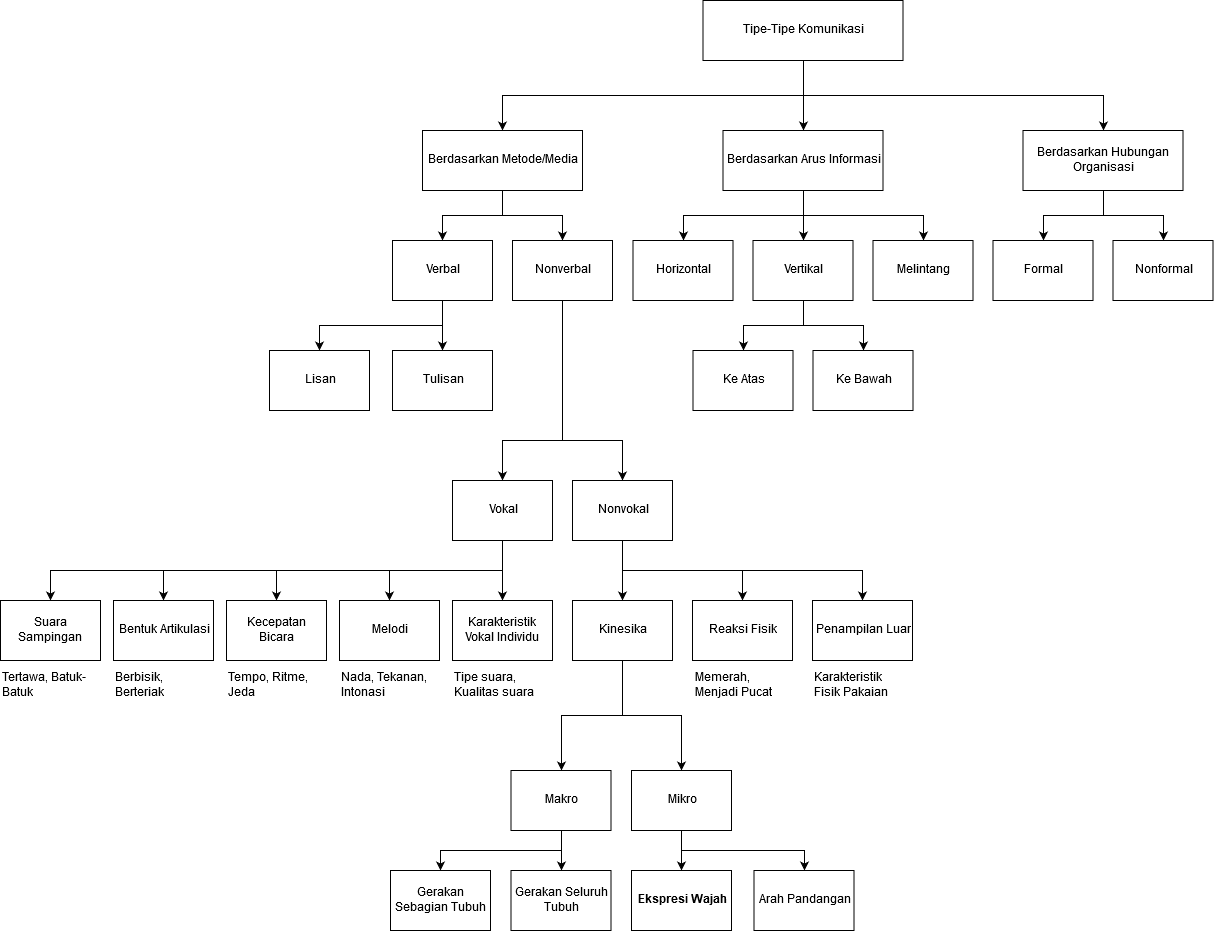
\includegraphics[width=14cm]{gambar/tipe_tipe_komunikasi.png}
    \caption[Pembagian Model-Model Komunikasi]{Pembagian Model-Model Komunikasi (\protect\shortciteNP{surkamp2014non};\\www.businesscommunicationarticles.com)}
    \label{fig:tipekomunikasi}
\end{figure}

Antara emosi, \textit{mood} dan perasaan, memiliki definisi yang berbeda di kalangan para ahli. Beberapa di antara mereka membedakannya. Dalam membandingkan emosi dan \textit{mood}, \shortciteA{ekman1994nature} menyatakan bahwa 1) \textit{mood} berlangsung lebih lama, 2) \textit{mood} lebih mudah terprovokasi, 3) \textit{mood} lebih sulit untuk dimodulasi, 4) \textit{mood} tidak memiliki ekspresi wajah unik sendiri, dan 5) \textit{mood} lebih sulit disadari penyebabnya dibandingkan dengan emosi.

Dalam kaitan emosi dengan perasaan/sentimen, \shortciteA{freedman2017emotions} menyatakan bahwa perasaan merupakan campuran dari emosi dan bertahan lebih lama. Perasaan muncul ketika membiarkan emosi, yang biasanya hanya bertahan selama enam detik. Menurut \shortciteA{perez2018emotions}, sentimen akan tetap bertahan selama disadari dan dipikirkan. Berbeda dengan emosi, sentimen dikendalikan secara sadar oleh pikiran. Sementara sebagian ahli membedakan perasaan dengan sentimen \shortcite{munezero2014they}. Meskipun konvensi dalam masalah ini belum terjadi, mereka bersepakat bahwa emosi bertahan dalam rentang waktu relatif lebih pendek.

Emosi merupakan sesuatu yang amat kompleks untuk dipahami bahkan secara mendalam. Emosi seseorang terbentuk atas berbagai faktor, seperti kepribadian \shortcite{arnold1960emotion}, bahasa \shortcite{lutz1990language}, kemampuan adaptasi \shortcite{smith1990emotion}, kultur \shortcite{kitayama1994emotion}, kondisi kesehatan \shortcite{pennebaker1995emotion}, kemampuan pengambilan keputusan \shortcite{schwarz2000emotion}, harapan \shortcite{kenny2003action}, motivasi \shortcite{bradley2007emotion} dan lain-lain. Seseorang dapat memahami signifikansi dan nilai dari sebuah emosi jika dia pernah mengalaminya sendiri \shortcite{mun2019knowing}.

Emosi merupakan sesuatu yang abstrak bagi orang lain. Akan tetapi, pada umumnya, emosi memiliki bentukan yang dapat diamati. Secara alami, emosi membentuk perilaku temporal seseorang \shortcite{baumeister2007emotion}. Bentukan tersebut hanya diakui akurat jika hal itu bersifat evaluatif \shortcite{mun2019knowing}.

Pengenalan emosi dapat dilakukan dengan berbagai teknik seperti melalui pengenalan ekspresi wajah \shortcite{canedo2019facial}, ucapan \shortcite{khalil2019speech}, tulisan \shortcite{seyeditabari2018emotion} atau sinyal-sinyal lain \shortcite{wagh2019electroencephalograph}. Masing-masing pendekatan tersebut dianggap representatif dalam pemodelan pengenalan emosi yang presisi dan akurat.

Pengenalan emosi melalui ekspresi wajah sendiri belum mampu mencerminkan emosi secara tepat dan utuh \shortcite{fernandez2013emotion}. Namun sejauh ini, pengenalan emosi melalui ekspresi wajah dinilai paling akurat. Sebab sebagian besar komunikasi adalah bersifat nonverbal \shortcite{lapakko2007communication,mehrabian1967decoding,mehrabian1967inference}.

\begin{figure}[t]
    \centering
    \begin{subfigure}[t]{6cm}
        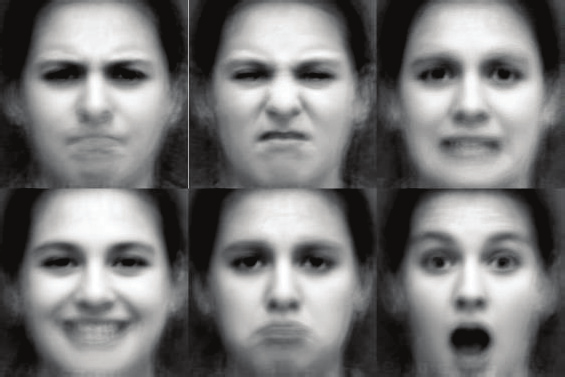
\includegraphics[width=6cm]{gambar/rerata_ekspresi_wajah_barat.png}
        \caption{}
    \end{subfigure}
    ~~~
    \begin{subfigure}[t]{6cm}
        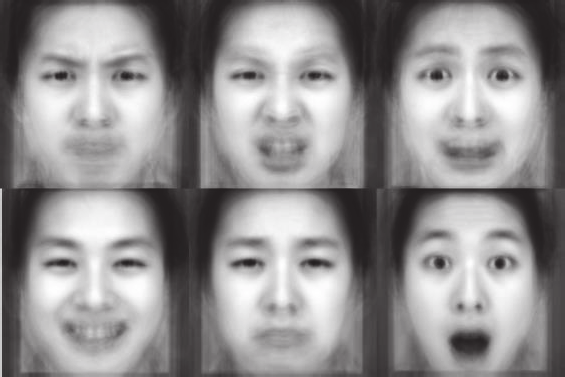
\includegraphics[width=6cm]{gambar/rerata_ekspresi_wajah_asia.png}
        \caption{}
    \end{subfigure}
    \caption[Perbedaan Rerata Pola Ekspresi Wajah Orang (a) Barat dan (b) Asia dalam Enam Kelas Emosi Berbeda]{Perbedaan Rerata Pola Ekspresi Wajah Orang (a) Barat dan (b) Asia dalam Enam Kelas Emosi Berbeda \protect\shortcite{benitez2017analysis}}
    \label{fig:rerataekspresiwajah}
\end{figure}

\begin{figure}[t]
    \centering
    \begin{subfigure}[t]{7.5cm}
        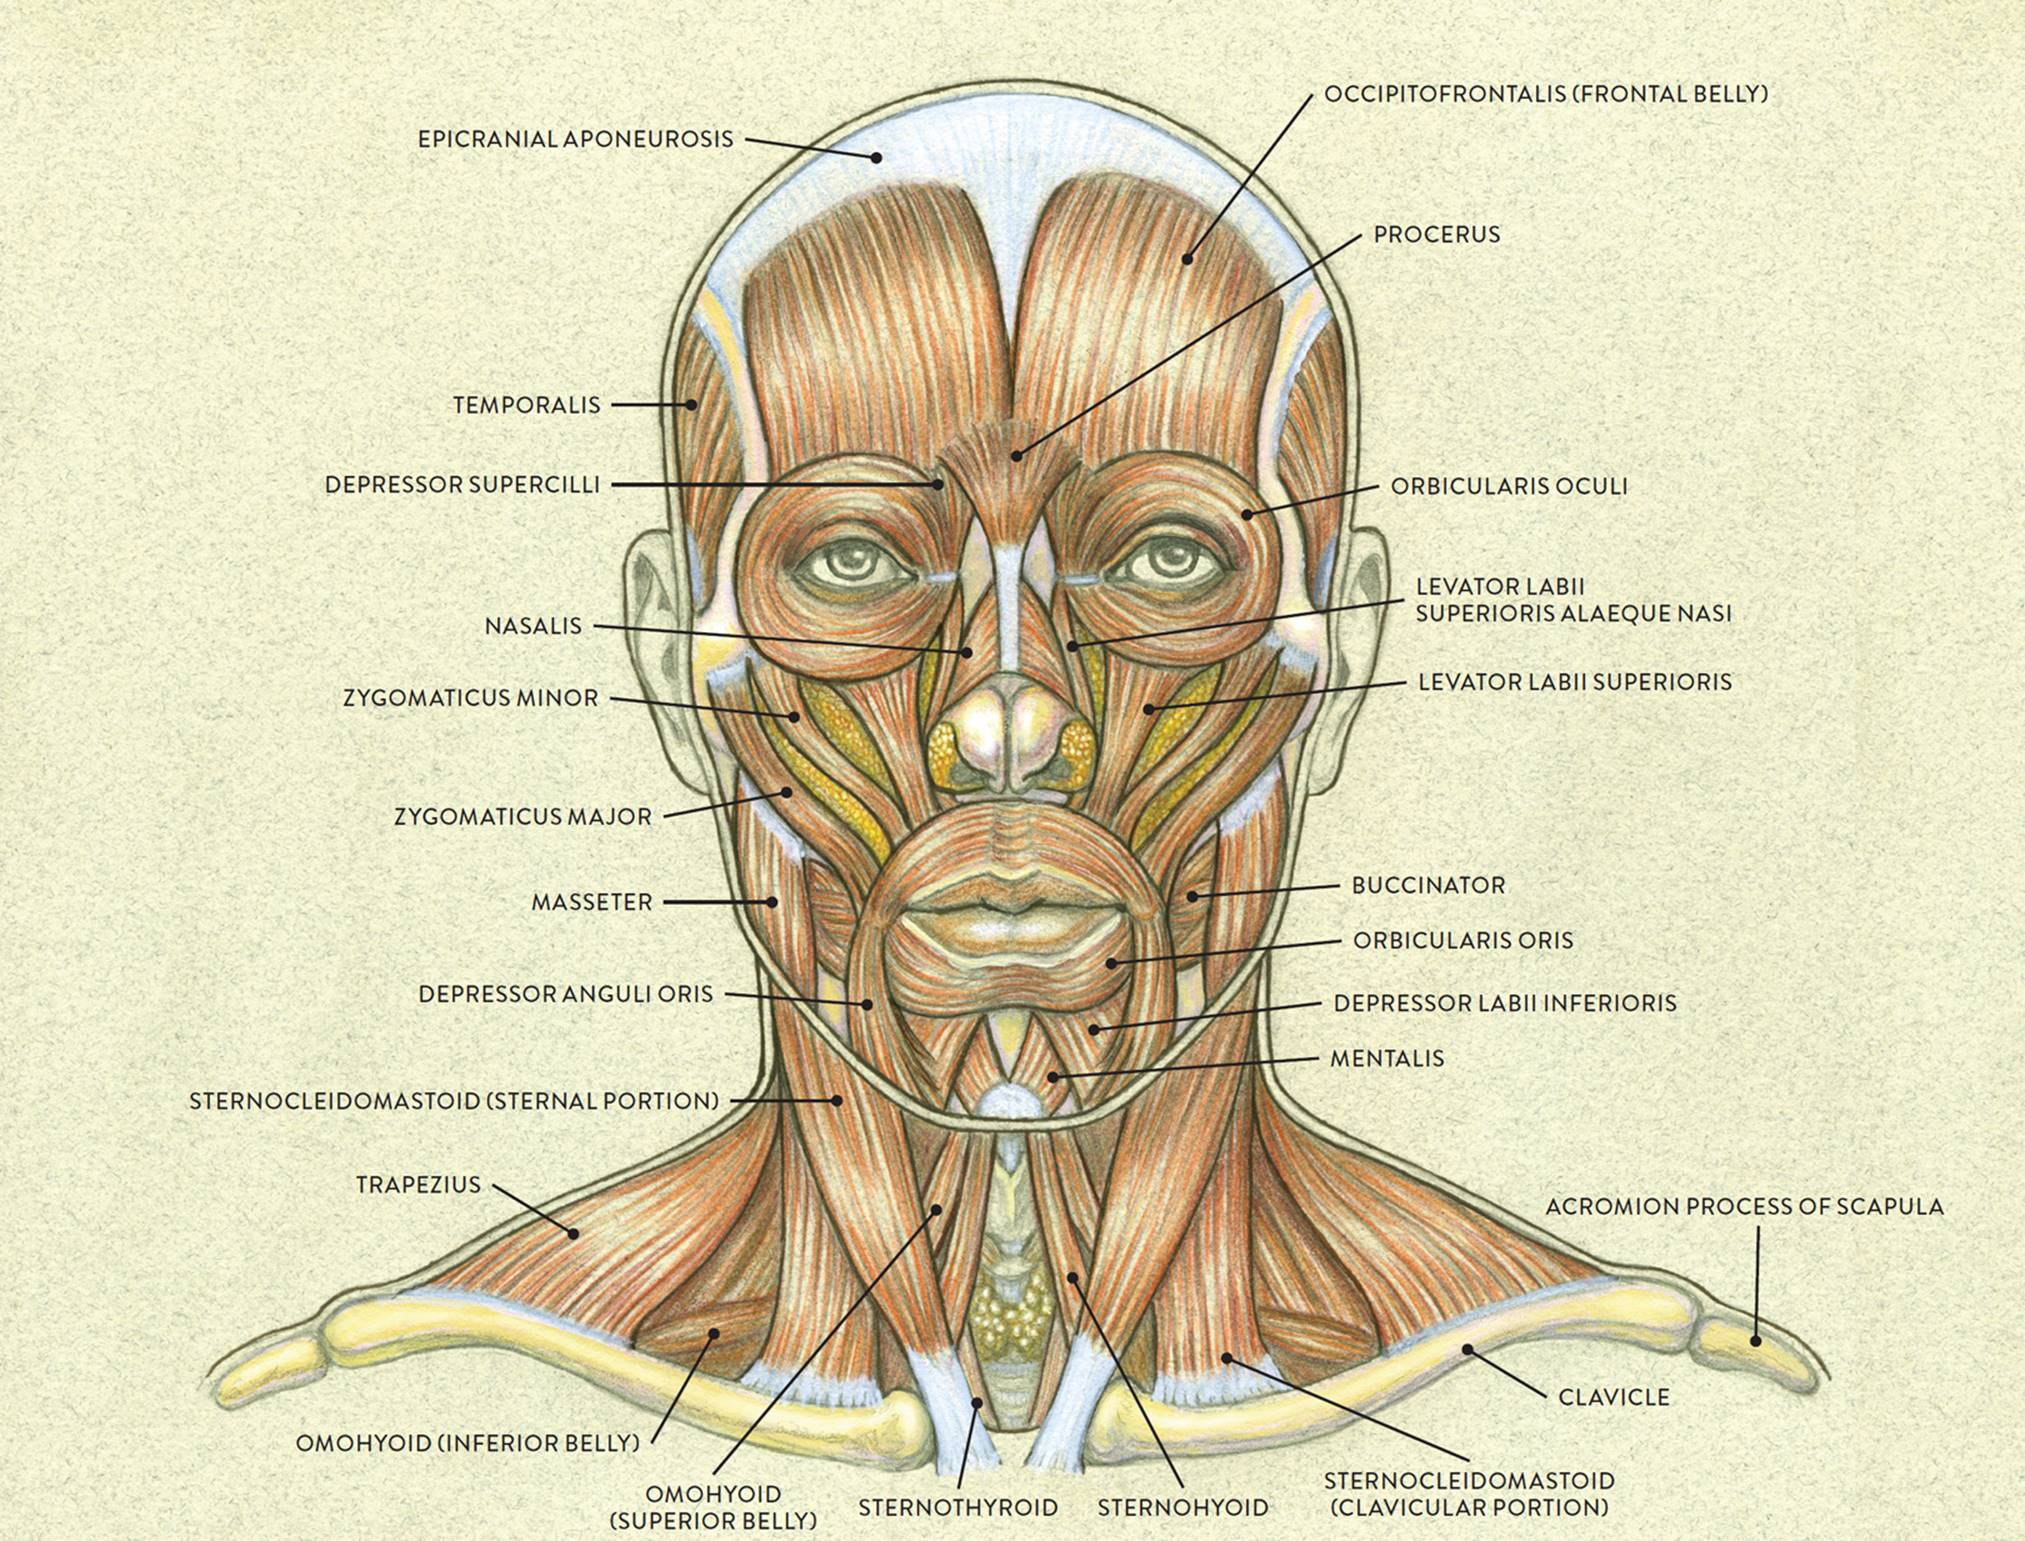
\includegraphics[width=7.5cm]{gambar/classic_human_anatomy_motion1.jpg}
    \end{subfigure}
    \begin{subfigure}[t]{4.5cm}
        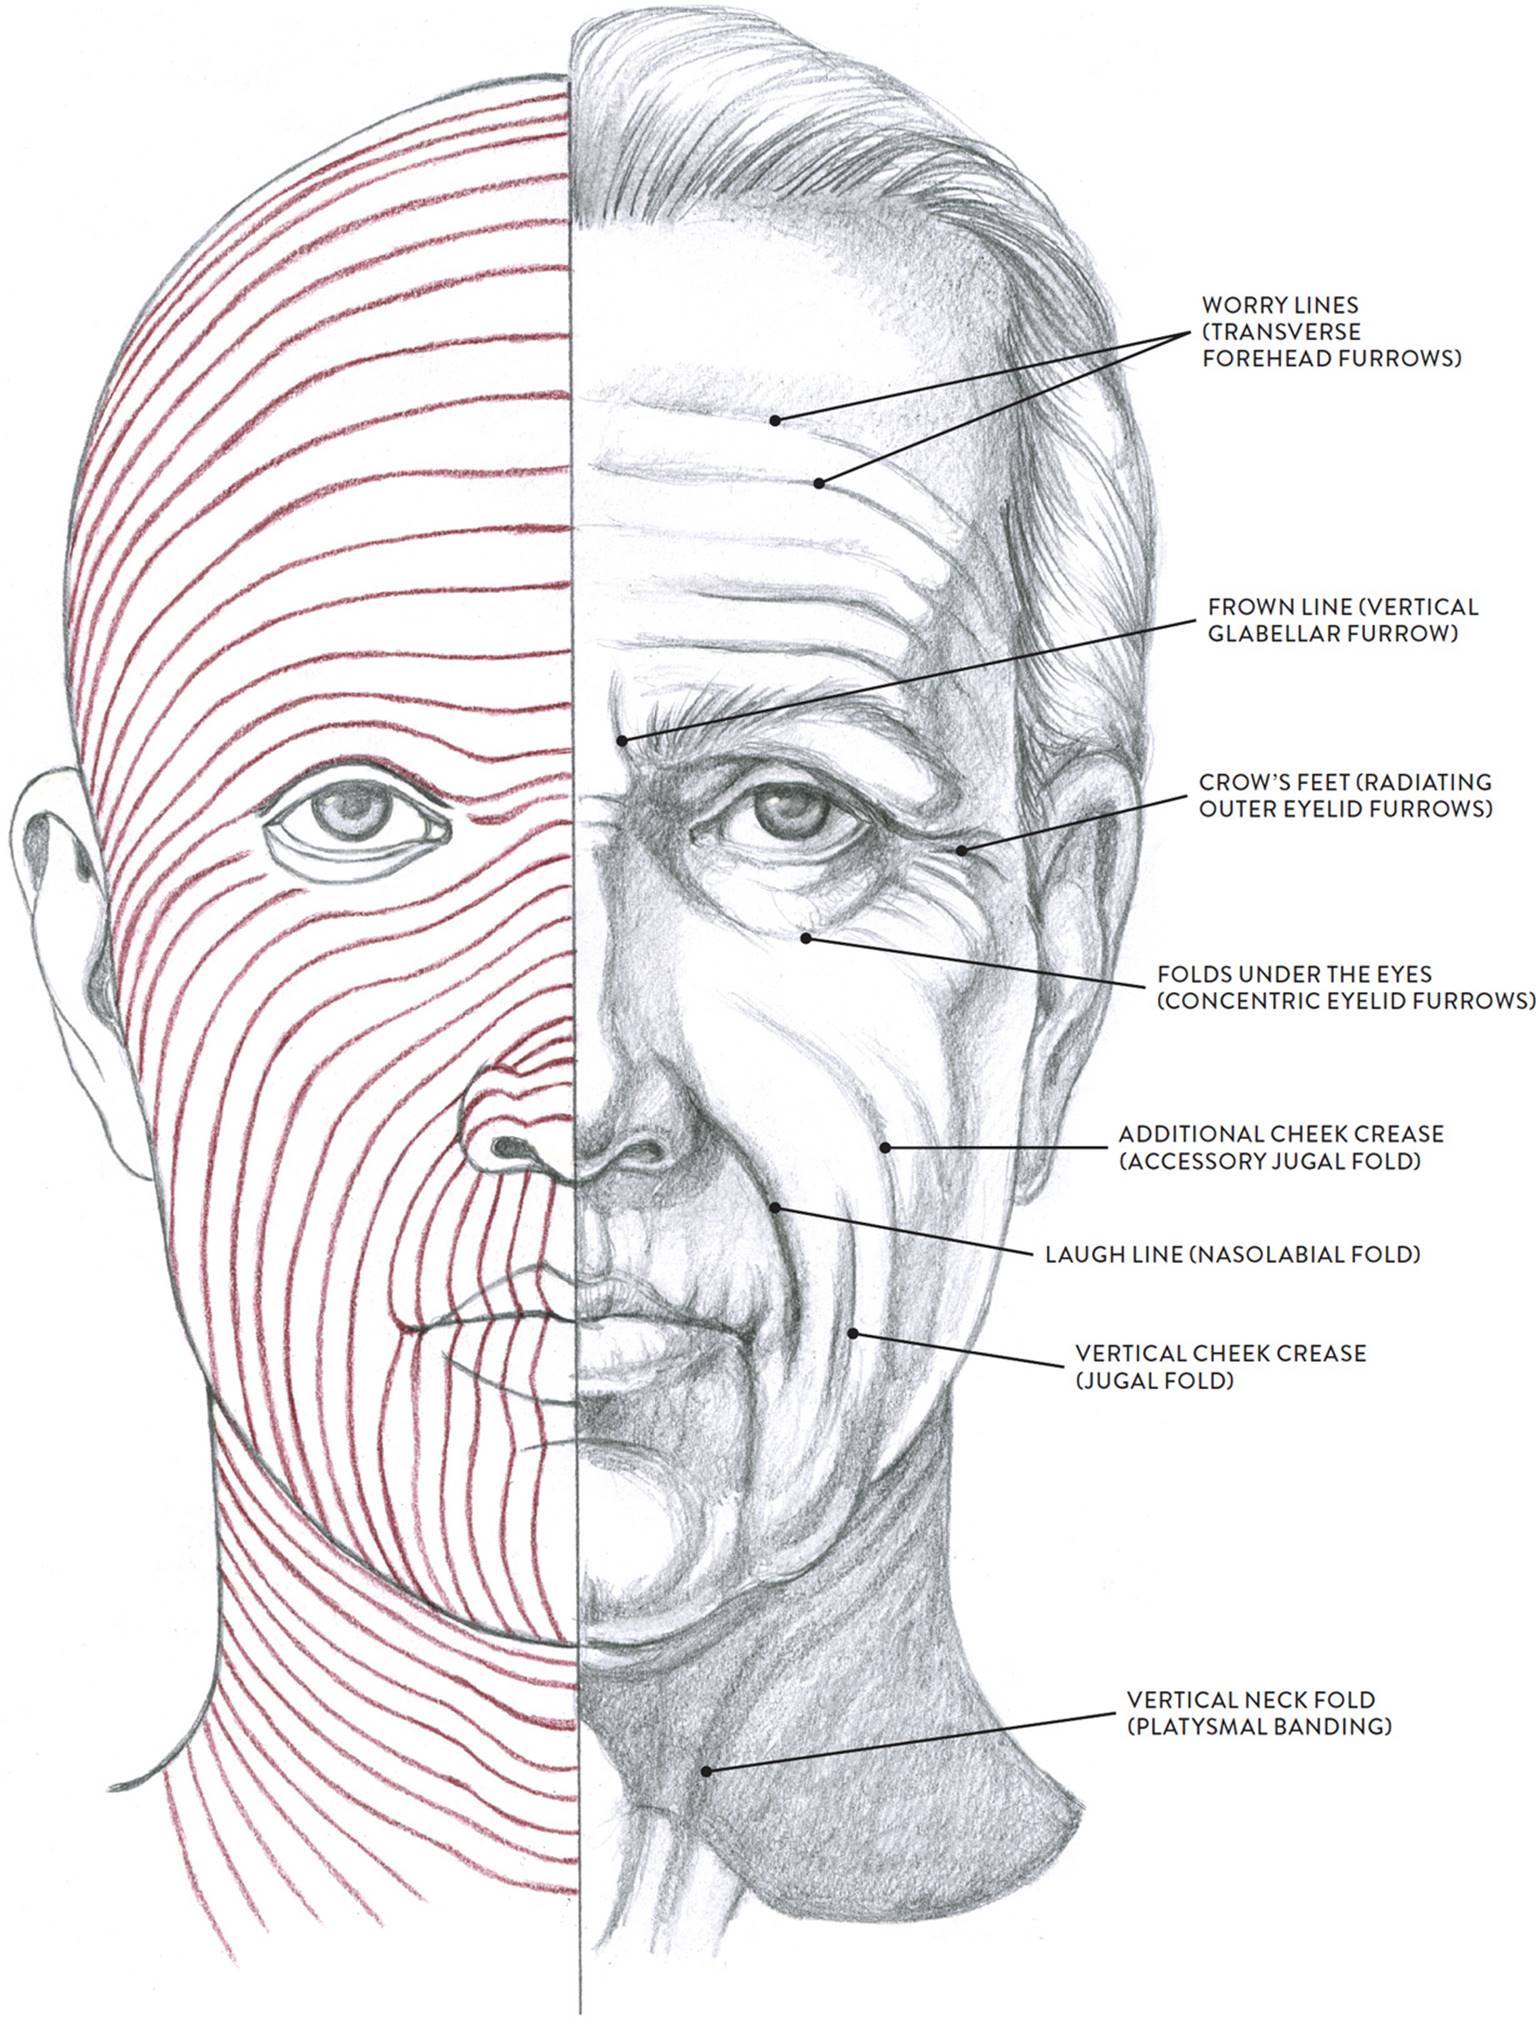
\includegraphics[width=4.5cm]{gambar/classic_human_anatomy_motion2.jpg}
    \end{subfigure}
    \caption[Otot-Otot Wajah Terkait Ekspresi Wajah]{Otot-Otot Wajah Terkait Ekspresi Wajah \protect\shortcite{winslow2015classic}}
    \label{fig:musclesface}
\end{figure}
Keuniversalan emosi masih terus diperdebatkan hingga sekarang ini \shortcite{gendron2014perceptions,hall2019nonverbal,jack2012facial}. \shortciteA{ekman1970universal} berpendapat bahwa sejumlah ekspresi wajah (\gls{sixbasicemotions}) bersifat universal, yaitu \textit{angry}, \textit{disgust}, \textit{fear}, \textit{happy}, \textit{sad}, \textit{surprise}, dan \textit{neutral}. Sebagian besar ilmuwan yang memenuhi kualifikasi \shortciteA{ekman2016scientists} menyetujui adanya bukti kuat pada keuniversalan emosi. Baru-baru ini terbukti bahwa \gls{sixbasicemotions} tidak berlaku antar kultur Asia dan Barat \shortcite{benitez2017analysis,benitez2018multicultural}. Gambar \ref{fig:rerataekspresiwajah} menunjukkan perbedaan yang cukup mendasar antara rerata pola ekspresi wajah dari kedua kultur tersebut.

Ekspresi wajah dapat dibedakan melalui lebih dari 10.000 kombinasi gerakan relatif lima belas otot bagian wajah (Gambar \ref{fig:musclesface}) \shortcite{ekman2004emotions,westbrook2019anatomy}. Kerutan kulit wajah karena usia, rona merah wajah, arah lirik dan kedipan mata serta ukuran pupil juga terlibat dalam pengenalan ekspresi wajah \shortcite{guo2013facial, kret2015emotional}.

\begin{figure}[t]
    \centering
    \begin{subfigure}[t]{6cm}
        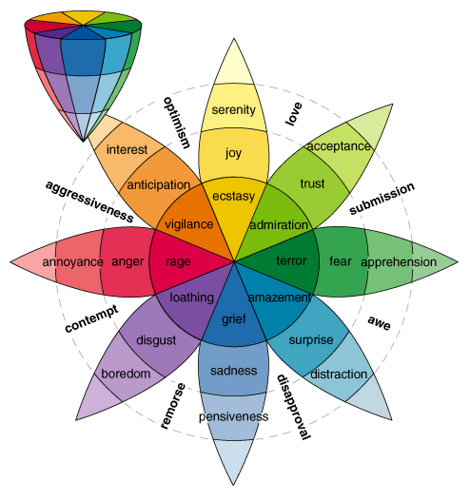
\includegraphics[width=6cm]{gambar/plutchik_wheel_emosi.jpg}
        \caption{\textit{Plutchik’s Wheel of Emotions} (https://www.theemotionmachine.com/\\classification-of-emotions/)}
        \label{fig:plutchikwheelemotions}
    \end{subfigure}
    \begin{subfigure}[t]{6cm}
        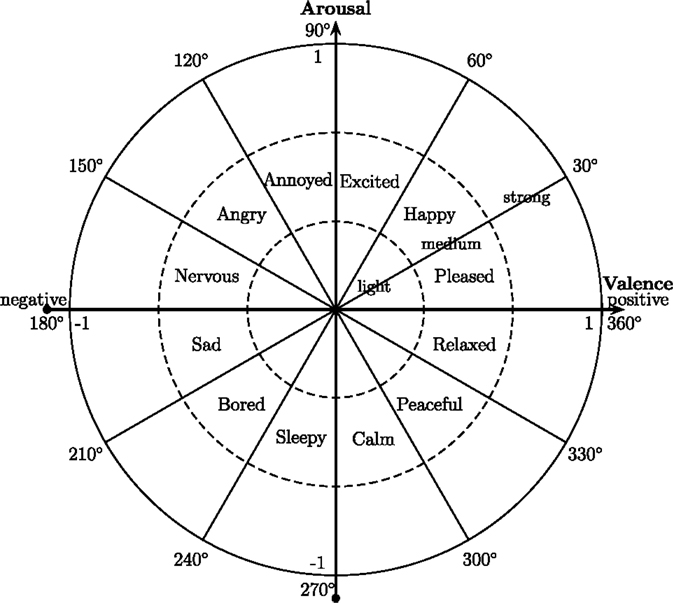
\includegraphics[width=6cm]{gambar/fuzzy_emosi.jpg}
        \caption{Lingkaran Emosi \textit{Fuzzy} \protect\shortcite{kowalczuk2016computational}}
        \label{fig:diagramemosifuzzy}
    \end{subfigure}
    \caption{Diagram Klasifikasi Emosi}
\end{figure}
Emosi tidak biner atau terdefinisi dengan baik, melainkan setiap emosi saling terhubung dan mempengaruhi satu sama lain menurut kedekatannya \shortcite{paiva2001safira}. Klasifikasi emosi tidak hanya terbatas pada model diskrit yang menghasilkan lima, enam atau 23 jenis emosi berbeda. Melalui pendekatan dimensional, \shortciteA{plutchik2013theories} memperkenalkan diagram emosi yang menghubungkan delapan jenis emosi dasar (Gambar \ref{fig:plutchikwheelemotions}). Melalui pendekatan \textit{fuzzy}, \shortciteA{kowalczuk2016computational} memperkenalkan lingkaran emosi dengan dua belas jenis emosi dasar (Gambar \ref{fig:diagramemosifuzzy}). Diagram pohon terstruktur \shortciteA{parrott2001emotions} bahkan mampu mendefinisikan hingga lebih dari seratus jenis emosi spesifik.

\newpage
\section{Penelitian Terkait}
\begin{figure}[t]
    \centering
    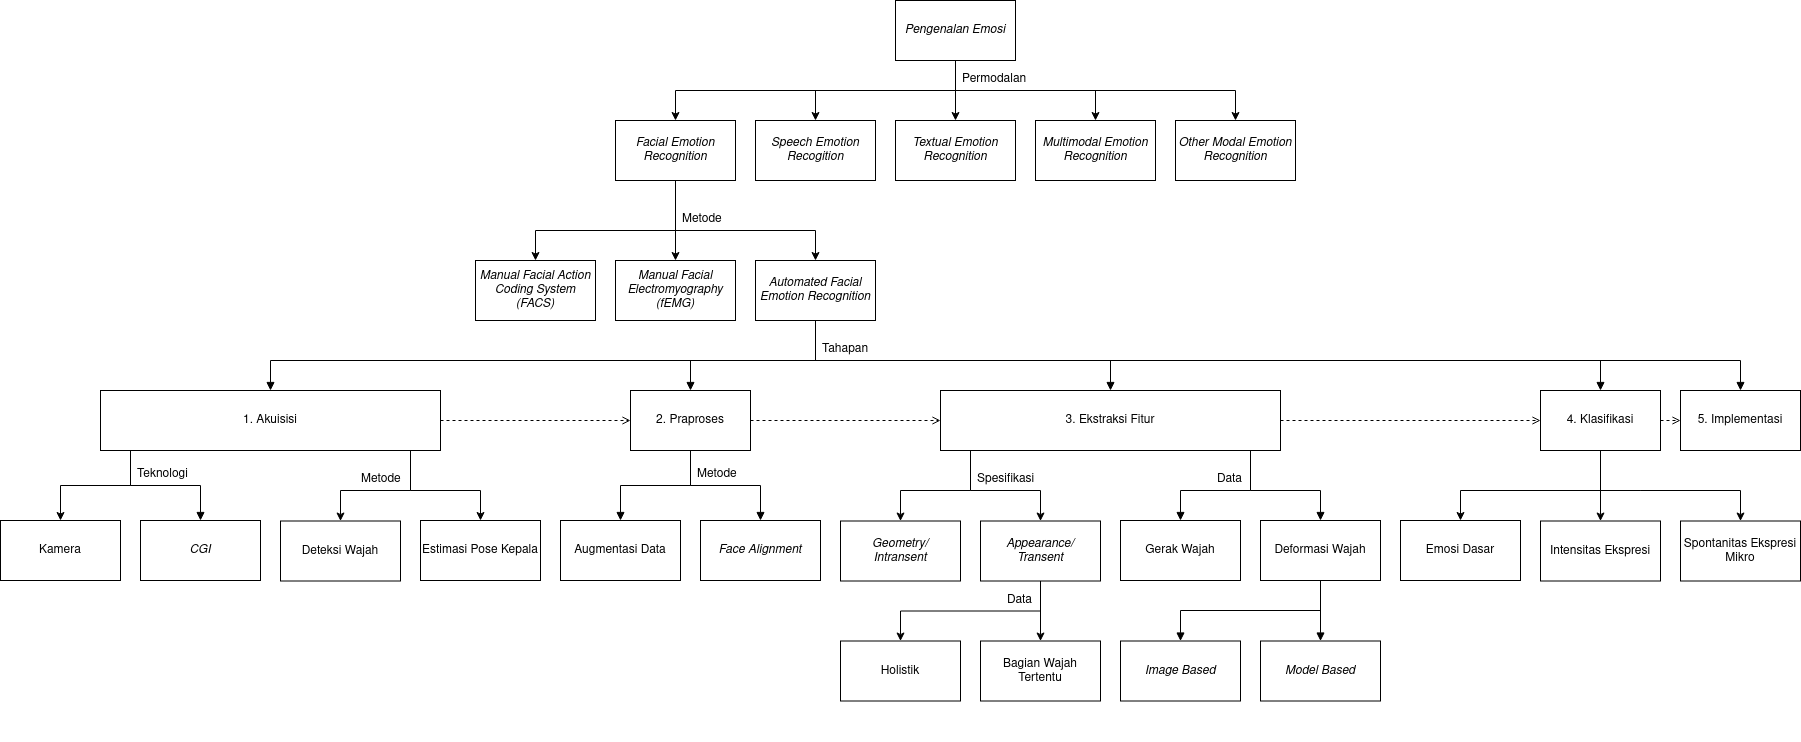
\includegraphics[width=14cm]{gambar/taksonomi_pengenalan_emosi.png}
    \caption[Taksonomi Pengenalan Emosi]{Taksonomi Pengenalan Emosi \protect\shortcite{sumathi2012automatic}}
    \label{fig:taksonomiemosi}
\end{figure}
Pengenalan emosi, terkait bidang ilmu komputer, memiliki domain penelitian yang sangat luas (Gambar \ref{fig:taksonomiemosi}). Berdasarkan jenis modal, pengenalan emosi dapat dilakukan baik melalui sinyal ucapan, tulisan, ekspresi wajah, sinyal digital ---seperti sinyal haptik dari \textit{drawing tablet} \shortcite{schrader2020linking}, sinyal aktifitas otak dari \textit{electroencephalogram} \shortcite{wagh2019electroencephalograph} dan sinyal tekanan dari \textit{keyboard} \shortcite{lv2008emotion}--- maupun kombinasi dari itu semua \shortcite{avots2019audiovisual,li2019fusion,mittal2019m3er}.

Pengenalan emosi melalui ucapan dapat dilakukan baik dengan pendekatan linguistik (tentang apa yang diucapkan) maupun paralinguistik (tentang bagaimana mengucapkannya) dalam komunikasi verbal. Dengan teknik-teknik pemrosesan sinyal, karakteristik unik tiap-tiap emosi dapat dikenali. Namun, belum ada konsensus mengenai set fitur standar untuk pengenalan ini. Sehingga menyulitkan pengevaluasian akurasi model pengenalan emosi dalam ucapan \shortcite{hook2019automatic,roy2020speech}. Bagaimanapun, hal ini merupakan tantangan terbesar bagi penelitian pengenalan emosi secara umum.

Pengenalan emosi melalui tulisan juga tergolong ke dalam kajian linguistik komputasi. Jika pengenalan emosi dalam ucapan cenderung meneliti mengenai gelombang bunyi dari wicara, maka pengenalan emosi dalam tulisan meneliti tentang tata bahasa yang terkandung dalam vektor-vektor kata baik dalam kumpulan frasa, kalimat maupun dokumen \shortcite{collobert2011natural,baali2019emotion}.

\begin{wrapfigure}{r}{4.6cm}
    \vspace{-0.5cm}
    \centering
    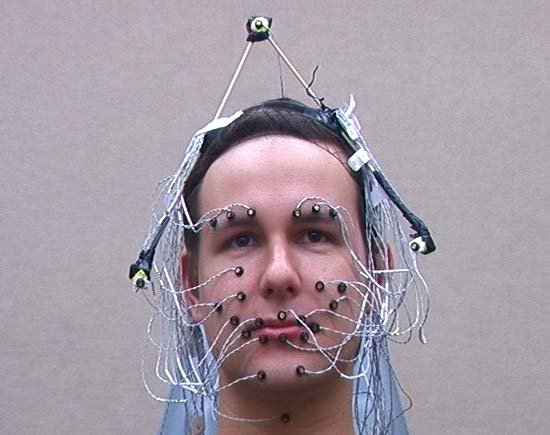
\includegraphics[width=4.5cm]{gambar/27_active_motion_capture_sensors.jpg}
    \caption[Contoh \textit{Facial Electromyography}]{Contoh \textit{Facial Electromyography} \protect\shortcite{gibert2010role}}
    \label{fig:contohfemg}
\end{wrapfigure}
Pengenalan emosi melalui ekspresi wajah menurut \shortciteA{wolf2015measuring} terbagi menjadi tiga metode, yaitu pelacakan aktivitas elektromiografi wajah, pengkodean aksi wajah dan rekognisi ekspresi wajah otomatis. Pelacakan aktivitas elektromiografi wajah atau \textit{facial electromyography} melibatkan penggunaan elektroda-elektroda yang dilekatkan pada permukaan wajah di titik-titik tertentu yang dianggap representatif (Gambar \ref{fig:contohfemg}). Sayangnya metode ini tidak dapat digunakan dalam situasi sosial sebab kompleksitas teknisnya. Namun, untuk mendeteksi aktivitas yang halus pada otot-otot wajah, metode ini sangat dapat diandalkan. Kesulitan yang dihadapi adalah menempatkan elektroda-elektroda tersebut pada posisi yang benar-benar tepat.

\begin{wrapfigure}{l}{4.7cm}
    \centering
    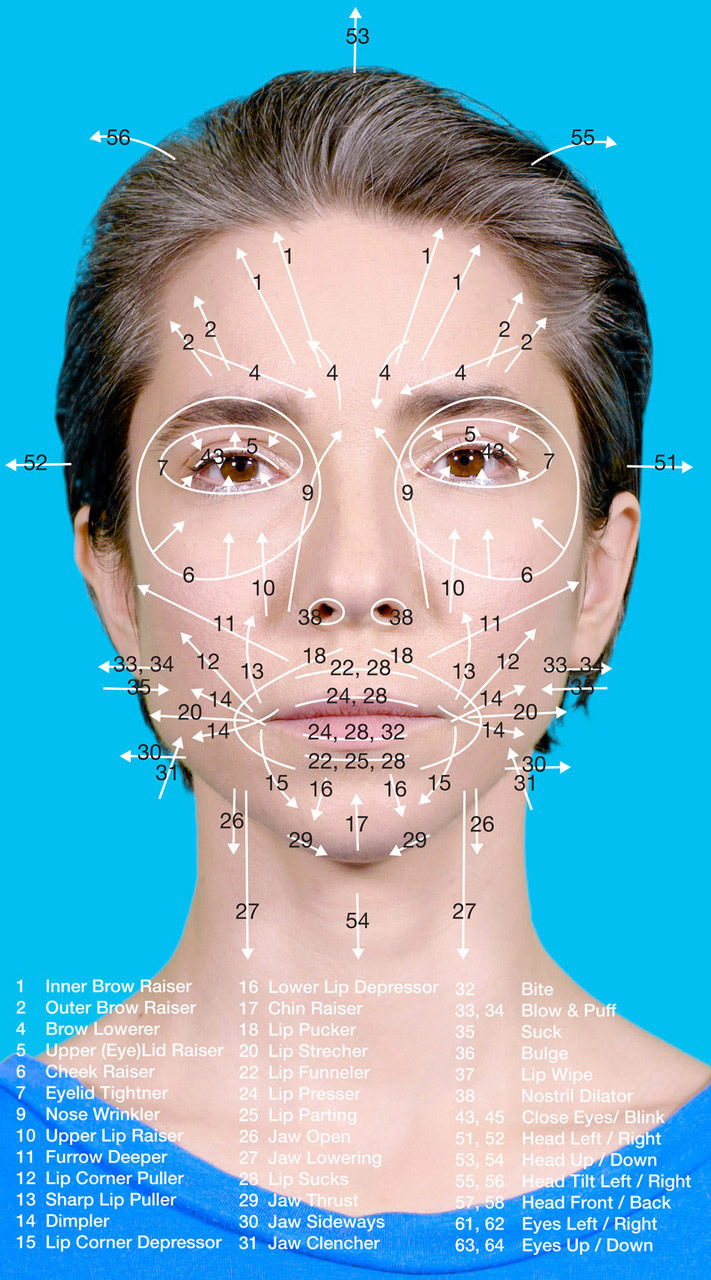
\includegraphics[width=4.7cm]{gambar/facs_coralie_vogelaar.jpg}
    \caption[Contoh \textit{Facial Action Units}]{Contoh \textit{Facial Action Units} (www.coralievogelaar.com)}
    \label{fig:contohfacs}
\end{wrapfigure}
Pengkodean aksi wajah atau \textit{facial action coding} \shortcite{ekman1997face} merupakan pengenalan emosi yang melibatkan analisis perubahan perilaku-perilaku otot-otot wajah yang kasat mata disebut sebagai unit aksi \textit{action units}. Unit-unit aksi ini didefinisikan secara manual, di antaranya adalah bagian kiri, kanan, luar dan dalam untuk tiap-tiap alis, mata, hidung, bibir dan mulut (Gambar \ref{fig:contohfacs}). Metode ini dapat meminimalkan bias oleh pengamat emosi. Namun proses analisis metode ini memerlukan bentukan emosi yang relatif kuat dan usaha manual yang banyak \shortcite{wolf2015measuring}. Dalam usaha meminimalkan waktu analisis pada perlakuan manual, pelacakan unit-unit aksi dikenali secara otomatis dengan pengukuran jarak relatif antar titik-titik wajah hasil deteksi tengara wajah atau \textit{facial landmarks} \shortcite{valstar2006fully}.

Pengenalan ekspresi wajah otomatis bekerja dengan cara menyandikan informasi ekspresi dari representasi wajah, baik informasi spasial dari tiap-tiap gambar statis maupun informasi hubungan temporal dari gambar-gambar sekuens, dengan bantuan \textit{machine learning}. Teknik \textit{machine learning} telah berkembang dari \textit{shallow learning} (di mana pemerolehan fitur-fitur wajah masih dilakukan secara manual) menjadi \textit{deep learning} (di mana pemerolehan fitur-fitur wajah diberikan seutuhnya kepada mesin). Teknik \textit{deep learning} telah terbukti jauh mengungguli metode-metode tradisional \shortcite{li2018deep}.

Pengenalan ekspresi wajah otomatis sangat bergantung pada kualitas dan kuantitas set data \textit{learning}\footnote{Penggunaan istilah set data \textit{learning} dalam konteks \textit{machine learning} mengacu kepada pengertian yang luas, yaitu mencakup set data \textit{training}, \textit{validation} dan \textit{test}.}. Maka dari itu, usaha memperoleh set data yang bagus menjadi tantangan tersendiri. Namun kekhawatiran pada pemerolehan set data ini tidak diperlukan lagi, sebab saat ini telah banyak orang dermawan yang bersusah payah untuk melakukannya. Set data tersebut sudah dilabeli dan disediakan gratis secara publik; penulis secara khusus bersyukur kepada para dermawan itu. Tinjauan mendetail mengenai beragam set data publik untuk pengenalan ekspresi wajah dapat ditemukan di \shortciteA{li2018deep}.

% TODO: bahas setiap komponen di taksonomi

\begin{figure}[t]
    \centering
    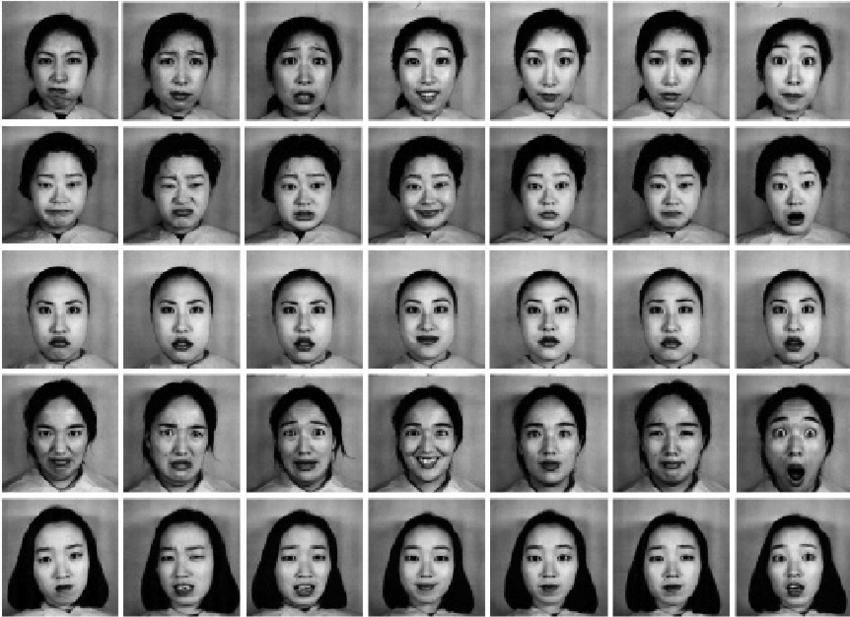
\includegraphics[width=14cm]{gambar/pratinjau_jaffe.jpg}
    \caption[Pratinjau Set Data JAFFE]{Pratinjau Set Data JAFFE \protect\shortcite{zhao2011facial}}
    \label{fig:pratinjaujaffe}
\end{figure}
Sebagian besar pengenalan ekspresi wajah otomatis memanfaatkan set data wajah frontal, contohnya JAFFE \shortcite{lyons1998coding}, CK+ \shortcite{lucey2010extended} dan EmotioNet \shortcite{fabian2016emotionet}. Gambar \ref{fig:pratinjaujaffe} memperlihatkan beberapa contoh gambar wajah frontal dari JAFFE. Mereka telah berhasil mencapai performa akurasi lebih dari 95\%. Model pengenalan ekspresi wajah melalui pendekatan teknik yang diusulkan oleh \shortciteA{zhou2019facial} bahkan mencapai akurasi sebesar 100\% untuk CK+. Namun, di samping kesulitan akuisisi data wajah frontal, model yang dikembangkan dengan set data wajah frontal menjadi tidak relevan pada penerapan di kondisi alam liar \shortcite{li2018deep}.

Pengenalan ekspresi wajah menggunakan set data wajah nonfrontal, contohnya FER-2013\footnote{Set data FER-2013 merupakan set data wajah nonfrontal publik yang paling populer digunakan dalam banyak penelitian pengenalan ekspresi wajah. Sejauh pengetahuan terbaik penulis, belum ada set data wajah nonfrontal lain yang tersedia secara publik.} \shortcite{goodfellow2013challenges}, hingga sekarang belum mencapai kepuasan berarti. Hasil survei penulis menuturkan bahwa akurasi tertinggi yang berhasil diraih saat ini untuk FER-2013 adalah 75,42\% \shortcite{georgescu2019local}. Untuk menemukan metode optimal yang mampu meningkatkan akurasi model pengenalan ekspresi wajah nonfrontal, maka penulis melakukan survei pada penelitian-penelitian terbaru. Penulis membatasi survei tersebut pada praproses, ekstraksi fitur dan model \acrshort{cnn} berikut performanya. Tabel \ref{tab:penelitiansota} memberikan gambaran mengenai hasil penerapan berbagai usulan metode penelitian dalam pengenalan emosi otomatis melalui ekspresi wajah.
\begin{table}[t]
    \caption{Penelitian Terkait}
    \label{tab:penelitiansota}
    \scriptsize
    \begin{tabular}{|C{1.4cm}|c|C{1.1cm}|C{2cm}|C{1.6cm}|C{1cm}|C{1cm}|c|}
        \hline
        \multicolumn{1}{|c|}{\multirow{2}{*}{Referensi}} & \multicolumn{1}{c|}{\multirow{2}{*}{Basis Data}} & \multicolumn{1}{C{1.1cm}|}{Tipe Jaringan} & \multicolumn{1}{C{2cm}|}{\multirow{2}{*}{Seleksi Data}} & \multicolumn{1}{c|}{\multirow{2}{*}{Praproses}} & \multicolumn{1}{C{1cm}|}{Ekstraksi Fitur} & \multicolumn{1}{c|}{\multirow{2}{*}{\textit{Classifier}}} & \multicolumn{1}{C{1cm}|}{Performa (\%)} \\
        \hline\hline
        \shortciteNP{georgescu2019local} & \multirow{15}{*}{\centering FER-2013} & \multirow{2}{*}{CNN, \textit{NE}} & \multirow{2}{*}{k-NN} & \multirow{4}{1.6cm}{\centering \textit{DA}} & \multirow{2}{1cm}{\centering CNNs + BOVW} & \multirow{2}{*}{\centering SVM} & \multirow{2}{*}{\centering 75,42} \\ % kutip FER+ jika diperlukan
        \cline{1-1}\cline{3-4}\cline{6-8}
        \shortciteNP{agrawal2020using} &  & \multirow{4}{*}{CNN} & \multirow{2}{2cm}{\centering 80\% set \textit{training}, 20\% set \textit{test}} &  & \multicolumn{2}{c|}{\multirow{2}{*}{CNN (16; 0,46M)$^\ast$}} & \multirow{2}{*}{65,23} \\
        \cline{1-1}\cline{4-8}
        \shortciteNP{engin2018face} &  &  & \multirow{11}{2cm}{\centering 28.709 set \textit{training}, 3.589 set \textit{validation}, 3.589 set \textit{test}} & \multirow{2}{*}{\textit{PN}} & \multicolumn{2}{c|}{\multirow{2}{*}{VGG-face}} & \multirow{2}{*}{67,60} \\
        \cline{1-1}\cline{3-3}\cline{5-8}
        \shortciteNP{kim2016fusing} &  & \multirow{5}{*}{CNN, \textit{NE}} &  & \multirow{5}{1.6cm}{\centering \textit{DA+FA+IN}} & \multicolumn{2}{c|}{\multirow{2}{*}{CNN (5; 2,4M)$^\ast$}} & \multirow{2}{*}{73,73} \\
        \cline{1-1}\cline{6-8}
        \shortciteNP{pramerdorfer2016facial} &  &  &  &  & \multicolumn{2}{c|}{\multirow{3}{2.2cm}{\centering CNN (10/16/33; 1,8M/1,2M/5,3M)$^\ast$}} & \multirow{3}{*}{75,20} \\
        \cline{1-1}\cline{3-3}\cline{5-8}
        \shortciteNP{zhang2015learning} &  & \multirow{4}{*}{CNN, \textit{MN}} &  & \multirow{2}{*}{\textit{FA}} & \multicolumn{2}{c|}{\multirow{2}{*}{CNN (6; 21,3M)$^\ast$}} & \multirow{2}{*}{75,10} \\
        \cline{1-1}\cline{5-8}
        \shortciteNP{devries2014multi} &  &  &  & \multirow{2}{*}{\textit{IN}} & \multicolumn{2}{c|}{\multirow{2}{*}{CNN (4; 12M)$^\ast$}} & \multirow{2}{*}{67,21} \\
        \hline
        \shortciteNP{qin2020facial} & \multirow{8}{*}{CK+} & \multirow{8}{*}{CNN, \textit{NE}} & \multirow{8}{*}{327 sekuens} & \multirow{2}{*}{\textit{FA+IN}} & \multicolumn{2}{c|}{\multirow{2}{*}{Filter Gabor + CNNs}} & \multirow{2}{*}{96,81} \\
        \cline{1-1}\cline{5-8}
        \shortciteNP{adil2019novel} & & & & \multirow{6}{*}{\textit{FRS}} & Filter Gabor & \multirow{2}{*}{SVM} & \multirow{2}{*}{92,19} \\
        \cline{1-1}\cline{6-8}
        \shortciteNP{ye2019facial} & & & & & \multicolumn{2}{c|}{\multirow{2}{*}{CNNs}} & \multirow{2}{*}{98,70} \\
        \cline{1-1}\cline{6-8}
        \shortciteNP{majumder2016automatic} &  &  &  &  & CNN + LBP & \multirow{2}{*}{SOM} & \multirow{2}{*}{98,95} \\
        \hline
    \end{tabular}
    {\raggedright
    \textit{DA---Data Augmentation}; \textit{FA---Face Alignment}; \textit{FRS---Facial Region Segmentation} \textit{IN---Illumination Normalization}; \textit{PN---Pose Normalization}; \textit{NE---Network Ensemble}; \textit{MN---Multitask Network}, \textit{CN---Cascaded Network}; \\
    $^\ast$(Jumlah total lapisan jaringan; jumlah total parameter \textit{training}).} \\
\end{table}

Perancangan desain model \acrshort{cnn} untuk pengenalan ekspresi wajah menghadapi dilema dalam upaya menghasilkan model yang efektif (dalam konteks akurasi) dan efisien (dalam konteks kompleksitas). Sehubungan dengan hal ini, \shortciteA{agrawal2020using} menjadi \textit{baseline} bagi penelitian penulis, yang mana model pengenalan ekspresi wajah yang diusulkan dapat menghasilkan akurasi seperti manusia sebesar 65,23\% \shortcite{goodfellow2013challenges} untuk FER-2013. Model yang diusulkan merupakan sebuah \textit{\acrlong{dcnns}} (\acrshort{dcnns}) murni dan sederhana ---tidak menggunakan \textit{dropout layer} dan \textit{fully connected layer}---. Dari dua model yang diberikan, penulis memilih \textit{model2} yang memiliki 464.183 parameter \textit{training}. Sebenarnya, perbedaan dari kedua model hanya terletak pada jumlah filter pada masing-masing lapisan konvolusi. Gambaran singkat arsitektur model yang digunakan dapat dilihat pada Gambar \ref{fig:arsiterturcnnbaseline}.
\begin{figure}[t]
    \centering
    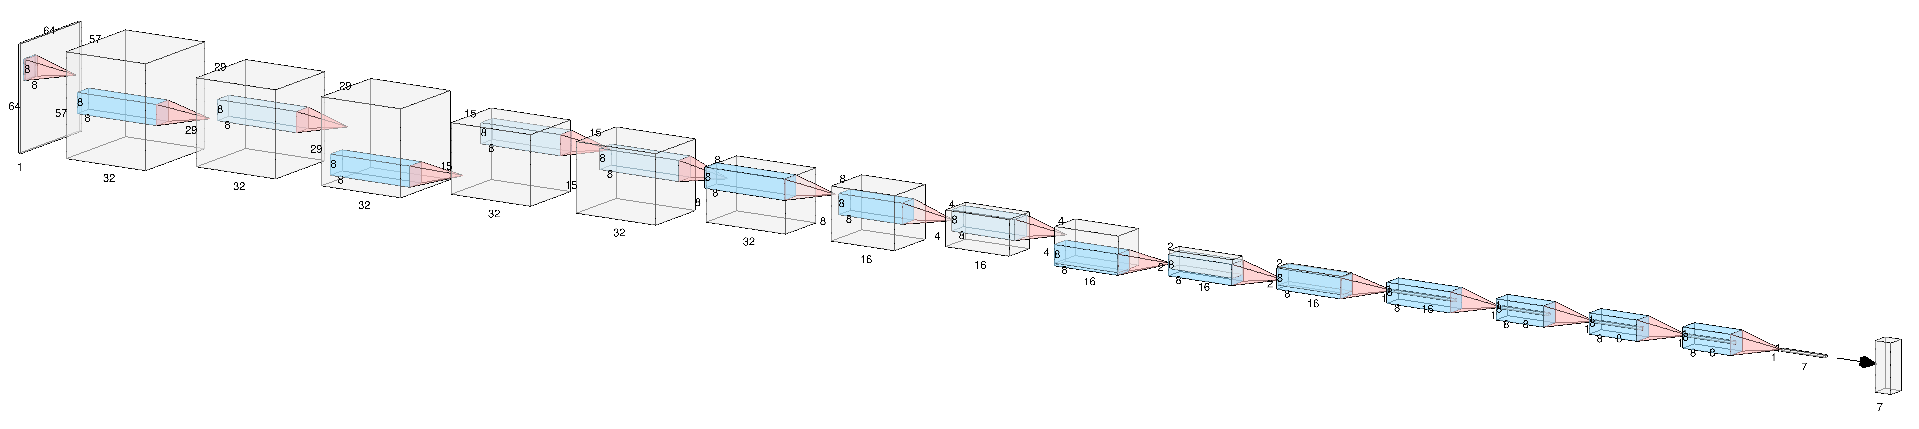
\includegraphics[width=14cm]{gambar/arsitektur_baseline_cnn.png}
    \caption[Arsitektur \acrshort{cnn} \textit{Baseline}]{Arsitektur \acrshort{cnn} \textit{Baseline} \shortcite{agrawal2020using}}
    \label{fig:arsiterturcnnbaseline}
\end{figure}

\textit{Network ensemble} adalah model jaringan yang terdiri beberapa jaringan. Model ini telah terbukti mengungguli model jaringan tunggal. Implementasi model ini mengharuskan tiap-tiap jaringan memiliki keragaman yang cukup dan didukung oleh metode pemaduan yang tepat, yaitu antara lain:
\begin{enumerate}
    \item \textit{Majority voting}: kelas data prediksi ditentukan oleh suara terbanyak dari tiap-tiap jaringan;
    \item \textit{Simple average}: kelas data prediksi ditentukan oleh perhitungan rerata probabilitas dengan bobot yang sama dari tiap-tiap jaringan;
    \item \textit{Weighted average}: kelas data prediksi ditentukan oleh perhitungan rerata probabilitas dengan bobot yang berbeda dari tiap-tiap jaringan \shortcite{li2018deep}.
\end{enumerate}
Model ini diterapkan pada pengenalan ekspresi wajah oleh \shortciteA{kim2016fusing} dan \shortciteA{pramerdorfer2016facial} demi mendapatkan akurasi sebesar 73,73\% dan 75,2\% untuk FER-2013.

\textit{Multitask network} adalah model jaringan yang diusulkan untuk mentransfer pengetahuan dari tugas-tugas relevan dan mengurai faktor-faktor gangguan. Model ini telah digunakan oleh \shortciteA{devries2014multi} dan \shortciteA{zhang2015learning} pada pengenalan ekspresi wajah demi mendapatkan akurasi sebesar 67,21\% dan 75,10\% untuk FER-2013.

\textit{Cascaded network} adalah model jaringan yang memadukan berbagai modul untuk tugas berbeda secara sekuensial. Modul-modul tersebut masing-masing berkontribusi pada penyaringan faktor-faktor variasi berbeda yang tidak dibutuhkan pada pengenalan ekspresi wajah \shortcite{li2018deep}.

\textit{Generative Adversarial Network} (GAN) adalah model jaringan khusus untuk membangkitkan gambar-gambar sintesis yang realistis. Pada pengenalan ekspresi wajah, model ini digunakan oleh \shortciteA{lai2018emotion} untuk membangkitkan gambar wajah frontal dari set data wajah nonfrontal. Penjelasan mendetail tentang model-model jaringan ini dapat ditemukan di \shortciteA{li2018deep}.

Strategi memadukan \acrshort{cnn} dan ekstraksi fitur konvensional belakangan ini telah banyak dilakukan. Strategi ini terbukti dapat meningkatkan akurasi model pengenalan ekspresi wajah. \shortciteA{georgescu2019local}, melalui usaha memadukan fitur-fitur yang diperoleh secara otomatis dan manual, saat ini menjadi \textit{state-of-the-art} bagi pengenalan ekspresi wajah untuk FER-2013. Eksperimen dimulai dengan pemilihan sampel data menggunakan \textit{k-Nearest Neighbor} (k-NN) \shortcite{fix1951discriminatory}. Secara manual, fitur-fitur diperoleh menggunakan model \textit{bag-of-visual-word} (BOVW) \shortcite{ionescu2013local} yang terdiri dari tahap ekstraksi fitur menggunakan \textit{Scale-Invariant Feature Transform} (SIFT) \shortcite{lowe2004distinctive} dan tahap \textit{clustering} menggunakan \textit{k-means} \shortcite{leung2001representing}. Secara otomatis, ekstraksi fitur dilakukan menggunakan tiga model \acrshort{cnn}, yaitu VGG-13 \shortcite{barsoum2016training}, VGG-f \shortcite{chatfield2014return} dan VGG-face \shortcite{parkhi2015deep}. Setelah itu, vektor representasi fitur dari \acrshort{cnn} dan BOVW dirangkai, dinormalisasikan dan dilatih menggunakan model \textit{Dense-Sparse-Dense} (DSD) \shortcite{han2016dsd} dengan \textit{Support Vector Machine} (SVM) \shortcite{cortes1995support} sebagai \textit{classifier}.

\textit{Facial region segmentation} merupakan salah satu teknik \textit{cropping}, yang mana memisahkan beberapa daerah fitur gambar wajah sehingga menghasilkan set data baru (Gambar \ref{fig:segmentasi18}). \textit{Facial region segmentation} telah diterapkan untuk set data wajah frontal karena kelengkapan fitur-fiturnya. Pada \shortciteA{majumder2016automatic}, \textit{facial region segmentation} digunakan untuk memisahkan daerah mata kiri, mata kanan, hidung dan mulut sehingga menghasilkan set data baru. Set data baru tersebut diduplikasi dan dikenakan \textit{local binary pattern} (LBP) \shortcite{ojala1996comparative}. Kemudian set data baru sebelum dan setelah perkenaan LBP dilatih menggunakan \textit{network ensemble} dengan \textit{self-organizing map} (SOM) \textit{classifier} \shortcite{kohonen1990self}. Model tersebut dilatih pada CK+ demi menghasilkan akurasi sebesar 98,95\%. Pada \shortciteA{ye2019facial}, bagian-bagian wajah yang disegmentasi adalah dahi (pertengahan daerah kedua mata), kedua mata dan mulut. Bagian-bagian tersebut dilatih menggunakan \textit{network ensemble} secara individu dan menghasilkan akurasi sebesar 98,70\%.
\begin{figure}[t]
    \centering
    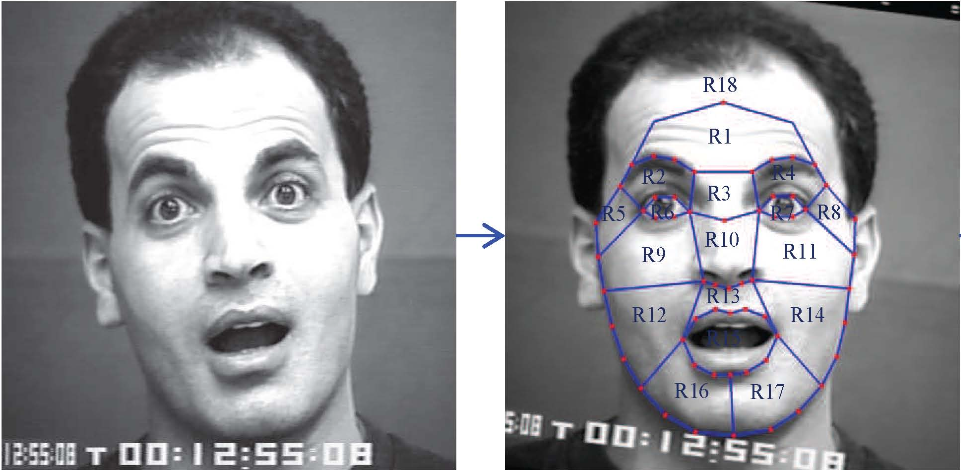
\includegraphics[width=14cm]{gambar/segmentasi_wajah_18.png}
    \caption[Segmentasi Delapan Belas Bagian Wajah]{Segmentasi Delapan Belas Bagian Wajah \protect\shortcite{ghimire2015facial}}
    \label{fig:segmentasi18}
\end{figure}

Filter Gabor merupakan salah satu filter konvolusi \acrshort{2d} yang populer digunakan dalam ekstraksi fitur berbagai tugas klasifikasi gambar menggunakan \acrshort{cnn}. Pada \shortciteA{qin2020facial}, pengenaan sejumlah filter Gabor pada set data input CK+ dibuktikan mampu meningkatkan kemampuan generalisasi \acrshort{cnn} dua kanal dan mencapai akurasi sebesar 96,81\%. Pada \shortciteA{adil2019novel}, penggunaan filter Gabor pada SVM \textit{classifier} menghasilkan akurasi sebesar 92,19\% untuk set data yang sama.

\section{Filter Gabor}
Filter Gabor adalah sebuah filter linear dari fungsi Gabor yang telah berhasil diterapkan di berbagai tugas pemrosesan gambar \shortcite{dunn1993optimal}, misalnya untuk sistem autentikasi biometrik \shortcite{aggrawal2016fingerprint,vijay2019highly}, deteksi kendaraan spesifik \shortcite{sara2019ambulance} dan identifikasi tulisan tangan \shortcite{baati2018towards,mohammed2019handwritten}.

\begin{figure}[t]
    \centering
    \begin{subfigure}[t]{12cm}
        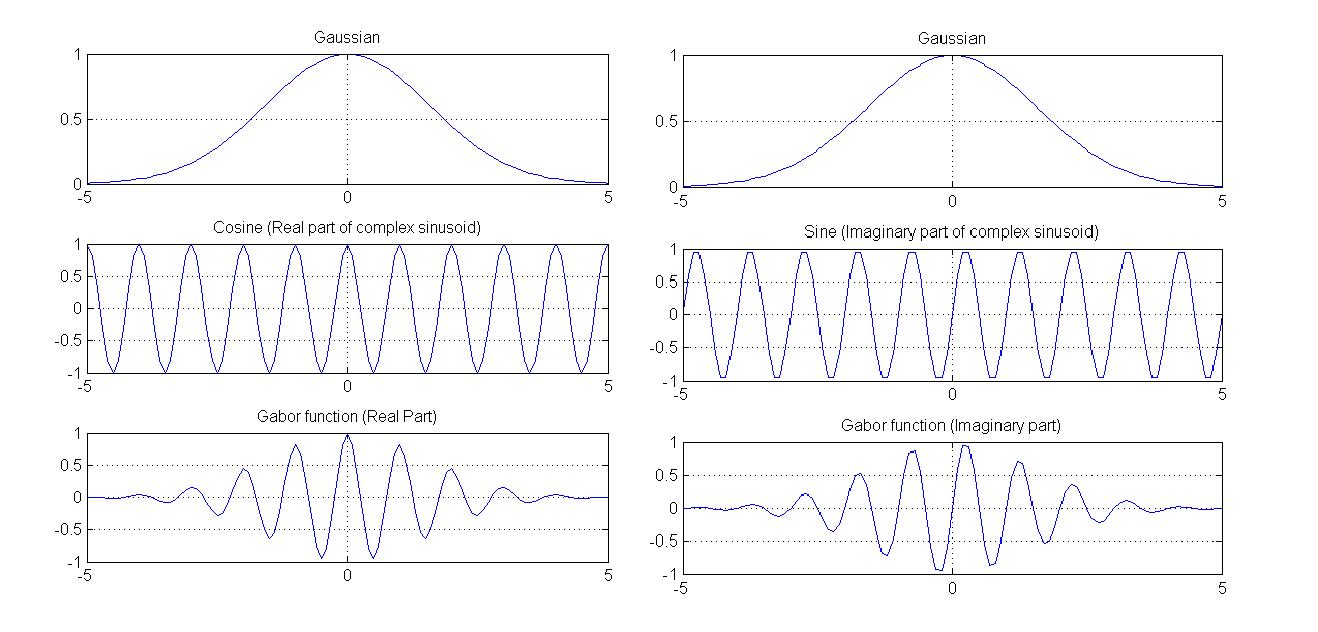
\includegraphics[width=12cm]{gambar/gabor2d.png}
        \caption[Fungsi Gabor pada Dimensi Dua]{Fungsi Gabor pada Dimensi Dua \protect\shortcite{viswanathan2014morlet}}
    \end{subfigure}
    \begin{subfigure}[t]{9cm}
        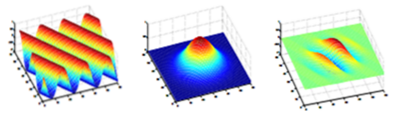
\includegraphics[width=9cm]{gambar/gabor3d.png}
        \caption[Fungsi Gabor pada Dimensi Tiga]{Fungsi Gabor pada Dimensi Tiga (https://medium.com)}
    \end{subfigure}
    ~~~
    \begin{subfigure}[t]{2.8cm}
        
\includegraphics[width=2.8cm]{gambar/filter_gabor.jpg}
        \caption[Filter Gabor]{Filter Gabor (https://think-piece.tistory.com)}
    \end{subfigure}
    \caption[Fungsi Gabor; Hasil Modulasi Sinyal Sinusoidal oleh Fungsi \textit{Gaussian}]{Fungsi Gabor; Hasil Modulasi Sinyal Sinusoidal oleh Fungsi \textit{Gaussian}}
    \label{fig:fungsigabor}
\end{figure}
Fungsi Gabor awalnya diperuntukkan dalam analisis sinyal saluran komunikasi, sebagai fungsi frekuensi terhadap waktu, guna mendapatkan esensi informasi \shortcite{gabor1946theory}. Fungsi ini diperluas menjadi fungsi \acrshort{2d} oleh \shortciteA{daugman1985uncertainty}, sebagai sebuah sinyal sinusoidal kompleks yang dimodulasi oleh fungsi Gaussian (Gambar \ref{fig:fungsigabor}), yang dinyatakan \shortcite{grigorescu20062} dalam (\ref{equ:gabor1}) dan (\ref{equ:gabor2}),
\begin{equation}
    g(x,y,\lambda,\theta,\psi,\sigma,\gamma) = \exp\left(\frac{-x'^2+\gamma^2y'^2}{2\sigma^2}\right) \exp\left(2\pi\frac{x'}{\lambda}+\psi\right)
    \label{equ:gabor1}
\end{equation}
\begin{equation}
    b = \log_2{\left(\frac{\frac{\sigma}{\lambda}\pi+\sqrt{\frac{\ln{2}}{2}}}{\frac{\sigma}{\lambda}\pi-\sqrt{\frac{\ln{2}}{2}}}\right)}, \frac{\sigma}{\lambda} = \frac{1}{\pi}\sqrt{\frac{\ln{2}}{2}}\left(\frac{2^b+1}{2^b-1}\right)
    \label{equ:gabor2}
\end{equation}
dimana,
\begin{description}[align=parleft,labelwidth=1cm]
    \item[$x'$] $= x\cos(\theta) + y\sin(\theta),$
    \item[$y'$] $= -x\sin(\theta) + y\cos(\theta),$
    \item[$\lambda$] $= \parbox[t]{11.3cm}{panjang gelombang faktor cosinus dari fungsi Gabor dengan nilai bilangan riil yang valid 2--256 piksel,}$
    \item[$\theta$] $= \parbox[t]{11.3cm}{orientasi normal terhadap garis paralel fungsi Gabor dengan nilai bilangan riil yang valid 0--80\degree,}$
    \item[$\psi$] $= \parbox[t]{11.3cm}{fase {\itshape offset} faktor kosinus dari fungsi Gabor dengan nilai bilangan riil yang valid -180\degree\ hingga 180\degree,}$
    \item[$\sigma$] $= \parbox[t]{11.3cm}{standar deviasi faktor {\itshape Gaussian} yang nilainya ditentukan oleh parameter $\lambda$ dan $b$,}$
    \item[$\gamma$] $= \parbox[t]{11.3cm}{rasio aspek spasial atau eliptisitas faktor {\itshape Gaussian} dengan nilai terletak antara 0,23 dan 0,92,}$
    \item[$b$] $= \parbox[t]{11.3cm}{{\itshape bandwidth} frekuensi spasial dari filter dengan nilai terletak antara 0,4 dan 2,5 oktaf.}$
\end{description}

Dalam pemrosesan gambar, pertama-tama, bank filter Gabor (Gambar \ref{fig:contohfiltergabor}) dibuat melalui konfigurasi unik berbagai parameter dalam (\ref{equ:gabor1}) dan (\ref{equ:gabor2}). Selanjutnya konvolusi dilakukan melalui perkalian dot matriks antara $m$ filter Gabor dengan $n$ input gambar sehingga menghasilkan $m \times n$ \textit{feature maps} (Gambar \ref{fig:contohkonvolusigabor}).
\begin{figure}
    \centering
    \begin{subfigure}[t]{6.5cm}
        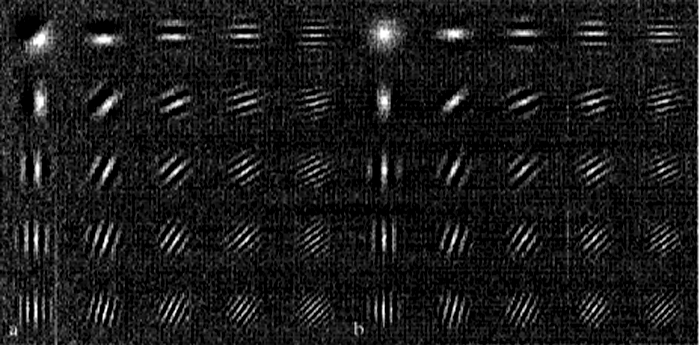
\includegraphics[width=6.5cm]{gambar/filter2_gabor.png}
        \caption[Contoh-Contoh Filter Gabor]{Contoh-Contoh Filter Gabor\\(https://www.cs.auckland.ac.nz)}
        \label{fig:contohfiltergabor}
    \end{subfigure}
    ~~~
    \begin{subfigure}[t]{6cm}
        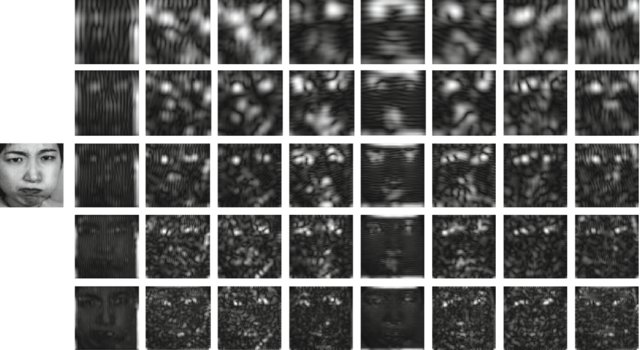
\includegraphics[width=6cm]{gambar/hasil_filter2_gabor.jpg}
        \caption[Contoh-Contoh Hasil Konvolusi oleh Filter Gabor]{Contoh-Contoh Hasil Konvolusi oleh Filter Gabor \protect\shortcite{dahmane2015conditional}}
        \label{fig:contohkonvolusigabor}
    \end{subfigure}
    \caption{Contoh Filter Gabor dan Hasil Konvolusi oleh Filter Gabor}
    \label{fig:konvolusigabor}
\end{figure}

Representasi frekuensi dan orientasi dari filter Gabor ditemukan mirip dengan sistem visual beberapa mamalia, sehingga filter ini sangat cocok untuk analisis tekstur \shortcite{sivalingamaiah2012texture}. Oleh karena itu, komputasi transformasi kompleks sebab tidak ortogonal menjadi kelemahan utama filter ini. Sifatnya yang demikian menimbulkan redudansi koefisien dan informasi \shortcite{vyas2006automated}. Sehingga tidak cocok digunakan pada sistem waktu nyata. Hal ini memotivasi berbagai penelitian untuk mencoba melakukan optimasi tanpa kehilangan akurasi yang berarti (\shortciteNP{ilonen2005efficient}; \shortciteNP{amayeh2009accurate}; \shortciteNP{kugaevskikh2017comparison}).

\section{Filter Log-Gabor}
\shortciteA{nava2011comparison} menyebutkan bahwa fungsi log-Gabor \shortcite{field87} dapat mengungguli performa fungsi Gabor pada pengenalan gambar yang memiliki tekstur yang kompleks. Dengan asumsi bahwa ekspresi wajah terbentuk dari kombinasi berbagai otot wajah yang menghasilkan tekstur kulit wajah yang kompleks, fungsi log-Gabor diharapkan dapat meningkatkan performa model rekognisi emosi. Fungsi log-Gabor dapat dirumuskan \shortcite{walia2016boosting} ke dalam (\ref{equ:loggabor}),
\begin{equation}
    g(r,\theta) = \exp{\left(\frac{-\log^2{\left(\frac{r}{f_0}\right)}}{2\sigma^2_r}\right)} \exp{\left(\frac{-(\theta-\theta_0)^2}{2\sigma^2_\theta}\right)},
    \label{equ:loggabor}
\end{equation}
% \begin{center}
%     dengan
% \end{center}
\begin{equation}
    f_0 = \text{wav}\times\text{scaleFactor}^n
\end{equation}
dimana,
\begin{description}[align=parleft,labelwidth=2cm]
    \item[$(r, \theta)$] $= \parbox[t]{10.3cm}{koordinat polar}$
    \item[$f_0$] $= \parbox[t]{10.3cm}{frekuensi pusat filter}$
    \item[\normalfont{wav}] $= \parbox[t]{10.3cm}{panjang gelombang dari skala terkecil}$
    \item[\normalfont{scaleFactor}] $= \parbox[t]{10.3cm}{faktor skala antar filter terurut}$
    \item[$\theta$] $= \parbox[t]{10.3cm}{sudut orientasi filter}$
    \item[$\sigma_r$] $= \parbox[t]{10.3cm}{skala {\itshape bandwidth}}$
    \item[$\sigma_\theta$] $= \parbox[t]{10.3cm}{sudut {\itshape bandwidth}}$
\end{description}

% TODO: contoh filter log-gabor

\section{\textit{\acrlong{ml}}}
\textit{Learning} adalah fenomena ---yang disimpulkan dari perilaku--- yang dapat diamati di seluruh makhluk hidup, termasuk manusia, hewan \shortcite{beran2020animal} dan tanaman \shortcite{parise2020extended}, baik saat mereka terjaga maupun saat tidur. \textit{Learning} dapat terjadi sekalipun tanpa keterlibatan dari orang lain \shortcite{gross2015psychology}. \textit{Learning} berarti perubahan potensi perilaku yang relatif permanen akibat keteraturan di lingkungan pelaku \shortcite{de2013learning,haselgrove2016learning}.

Hewan dan tanaman belajar melalui hubungan antara peristiwa dan respons yang berdekatan (\textit{associative learning}). Sebagai contoh, seekor kucing yang mana selalu diberi makan oleh pemiliknya setiap kali mengeong di dapur belajar jika mengeong adalah cara untuk meminta dan mendapatkan makanan \shortcite{ramos2009animal}. Contoh lain, tanaman putri malu akan mengatup sedikit dalam menanggapi sentuhan ringan dan akan mengatup rapat dalam menanggapi stimulus taktil. Setelah beberapa kali dikenakan sentuhan ringan dan stimulus taktil, maka tanaman putri malu akan mulai mengatup rapat dalam menanggapi sentuhan ringan \shortcite{abramson2016learning}.

\textit{Machine learning} \shortcite{hebb1949organization} muncul akibat keinginan untuk mengenakan \textit{learning} kepada mesin, sehingga dia mampu berinteraksi dengan lingkungannya berdasarkan pengetahuan yang diperoleh dari pengalaman. Untuk itu, berbagai disiplin terkait dipelajari seperti statistika, model interaksi sel-sel otak, teori kontrol adaptif, model-model psikologi, kecerdasan buatan, dan model-model evolusi \shortcite{nilsson2005introduction}. Akan tetapi, bagaimanapun, hingga saat ini, konsep-konsep dan teknik-teknik \textit{machine learning} lebih banyak diperoleh dari statistika daripada disiplin lain \shortcite{mitchell2006discipline}.

Sebuah mesin dikatakan belajar jika sistem secara andal meningkatkan kinerja (yang diukur oleh metrik tertentu) secara otomatis pada tugas tertentu mengikuti pengalaman tertentu. Mesin tersebut harus mampu bekerja menurut arsitektur komputasi dan algoritma tertentu dalam memproses set data statistik untuk aplikasi dimana \shortcite{nilsson2005introduction,mitchell2006discipline}:
\begin{enumerate}
    \item Beberapa tugas memerlukan algoritma yang rumit untuk didesain secara manual. Atau dengan kata lain, hanya dapat ditentukan oleh pasangan input dan keluaran. Sebagai contoh, tidak ada seorang pun mampu menulis algoritma untuk melabeli foto-foto yang memuat dirinya, namun melakukannya adalah mudah bagi semua orang.
    \item Korelasi antar data tersembunyi dalam himpunan data yang besar dan kompleks. Sebagai contoh, pada kasus penipuan kartu kredit, akan sangat sulit bagi orang untuk menemukan pola penipuan secara manual dari data transaksi bank.
    \item Lingkungan operasional tidak terdefinisi secara komplet pada waktu desain. Sebagai contoh, toko buku daring yang mampu menyesuaikan diri dengan preferensi pembelian setiap akun pelanggan.
\end{enumerate}
Dengan syarat-syarat di atas, pemanfaatan \textit{machine learning} menjadi sangat luas dan beragam. \textit{Machine learning} dapat diterapkan dengan bijak hampir di setiap lini kehidupan manusia.

% \textit{Machine learning} tidak terbatas oleh masalah-masalah dengan bentukan data input tertentu. Sebaliknya, dia menerima hampir semua data konkret, mencakup data vektor, \textit{list}, set, matrix, gambar, video, graf, \textit{string} dan campuran dari itu semua \shortcite{smola2008introduction}. Tiap-tiap jenis data tersebut diolah dengan cara-cara yang berbeda.

% \begin{figure}
%     \centering
%     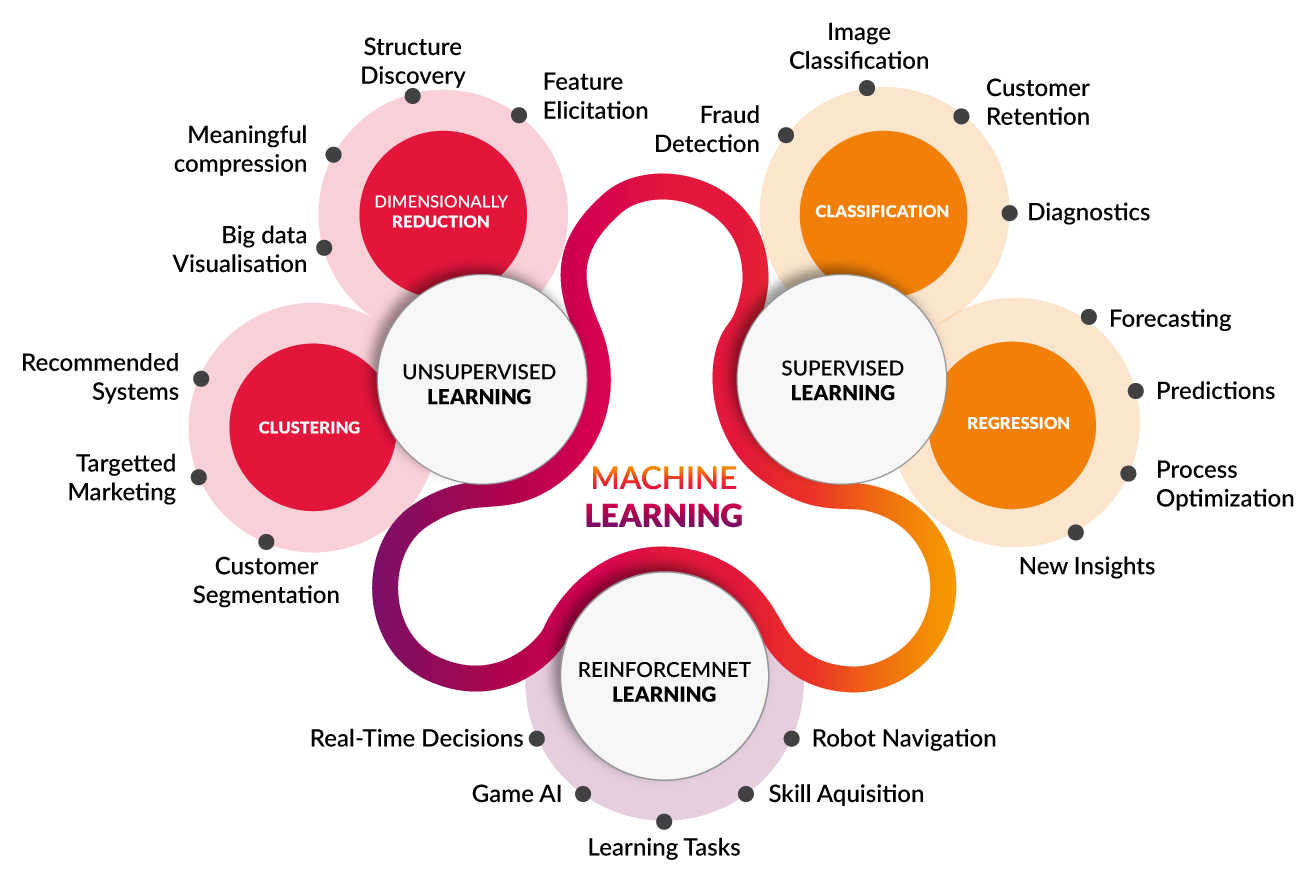
\includegraphics[width=12cm]{gambar/machine_learning_task.png}
%     \caption[Klasifikasi \textit{Machine Learning}]{Klasifikasi \textit{Machine Learning}\\(https://www.cognub.com)}
%     \label{fig:klasifikasiml}
% \end{figure}
% Tugas-tugas \textit{machine learning} dapat dibedakan menjadi \textit{supervised learning}, \textit{unsupervised learning} dan \textit{reinforcement learning} (Gambar \ref{fig:klasifikasiml}). \dots

% Problem-problem \textit{supervised learning}, berdasarkan keluarannya, dapat dibedakan menjadi klasifikasi dan regresi. Problem-problem klasifikasi, berdasarkan jumlahnya, dapat dibedakan menjadi \textit{binary classification} dan \textit{multiclass classification}. \dots

\subsection{\textit{\acrlong{ann}}}
\begin{figure}[t]
    \centering
    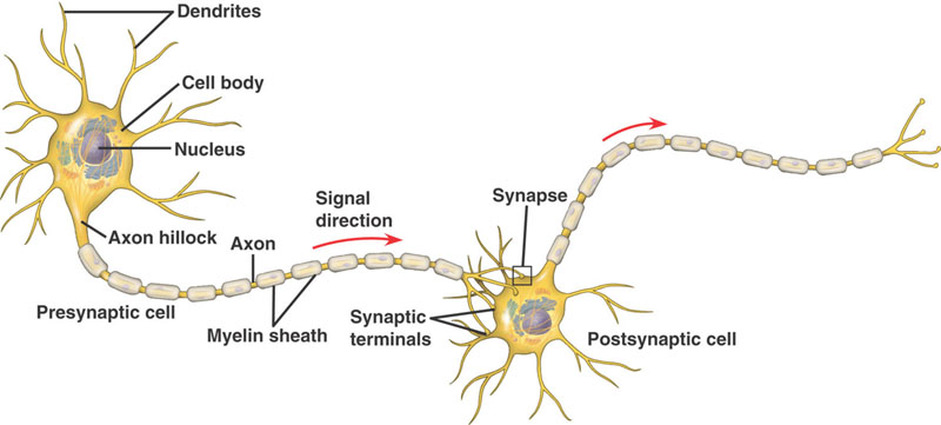
\includegraphics[width=10cm]{gambar/neuron.jpg}
    \caption[Struktur Neuron]{Struktur Neuron (https://mikerbio.weebly.com)}
    \label{fig:neuron}
\end{figure}
Otak manusia tersusun atas miliaran neuron yang saling berhubungan. Masing-masing neuron memiliki sel tubuh (soma), sejumlah dendrit dan sejumlah akson (Gambar \ref{fig:neuron}). Dendrit berfungsi untuk menerima sinyal dari akson lain pada neuron tetangga. Sinyal tersebut akan ditransmisikan melalui dari akson ke dendrit yang terkoneksi melalui sinapsis jika kekuatan sinyal tersebut di atas ambang batas tertentu. Melalui penyebaran dan interaksi sinyal-sinyal ini dalam anatomi neuron yang rumit, di mana melibatkan mekanisme nonlinear pada berbagai skala temporal dan spasial, pemrosesan informasi di otak berlangsung \shortcite{hines1997neuron,singh2001introduction}.

\textit{\acrlong{ann}} (\acrshort{ann}) mengacu pada model matematika yang memiliki arsitektur terdistribusi, yaitu terdiri atas soma (dapat dianalogikan) sebagai simpul/unit komputasi, sejumlah dendrit sebagai input, sejumlah akson sebagai keluaran dan sinapsis sebagai penyimpan informasi berupa bobot/parameter. Setiap simpul memiliki sebuah fungsi tertentu yang disebut \textit{perceptron} \shortcite{singh2001introduction,an2017electrical}. Secara umum, jaringan ini dapat digambarkan sebagai graf terarah yang terdiri dari lapisan input, lapisan tersembunyi dan lapisan target. Lapisan input terdiri dari $i$ buah simpul ditambah dengan sebuah simpul konstan yang selalu menghasilkan nilai bobot sama dengan satu. Di mana lapisan tersembunyi dapat terdiri dari satu atau lebih lapisan yang memiliki sejumlah simpul yang saling terhubung. Setiap lapisan tersembunyi dapat memiliki jumlah simpul yang beragam ditambah sebuah simpul bias yang tidak memiliki input dan menghasilkan sebuah konstanta. Kedalaman jaringan diukur dengan menjumlahkan banyak lapisan tersembunyi dan lapisan target. Besar jaringan diukur dengan menjumlahkan seluruh simpul pada setiap lapisan jaringan \shortcite{shalev2014understanding}.

\begin{figure}
    \centering
    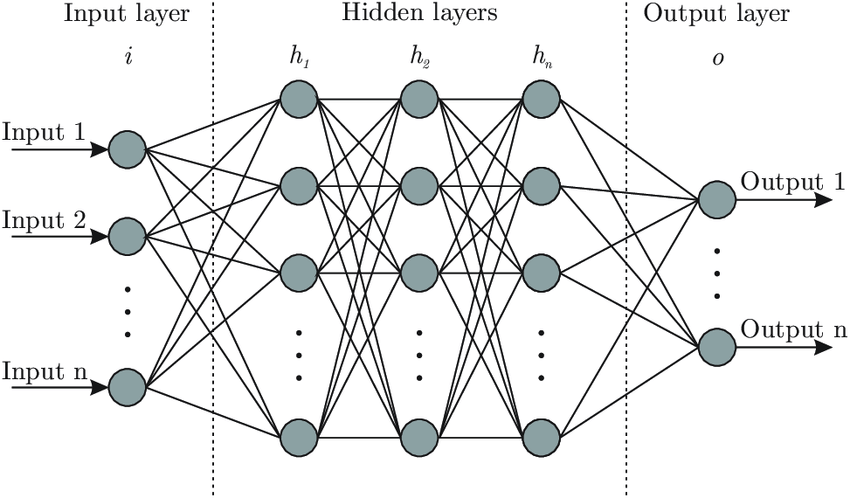
\includegraphics[width=10cm]{gambar/model_ann.png}
    \caption[Model \textit{\acrlong{ann}}]{Model \textit{\acrlong{ann}} \protect\shortcite{bre2018prediction}}
    \label{fig:modelann}
\end{figure}
Salah satu bentuk dari jaringan ini adalah \textit{feedforward multilayer perceptron}, di mana \textit{feedforward} berarti aliran data bergerak satu arah, dari input ke target/keluaran. Gambar \ref{fig:modelann} memperlihatkan jaringan \textit{feedforward} yang memiliki sejumlah input, tiga lapisan tersembunyi dan sejumlah target. Misalkan ($x_1, x_2, ..., x_i$) merupakan vektor input dan ($y_1, y_2, ..., y_m$) merupakan vektor target. Setiap simpul input terkoneksi dengan setiap simpul pada lapisan tersembunyi pertama dan setiap koneksi ini memiliki sebuah bobot $w_{i,j}$. Maka simpul ke-$j$ pada lapisan tersembunyi pertama, melalui fungsi aktivasi/transfer nonlinear tanh, melewatkan hasil penjumlahan bobot dari setiap inputnya, yaitu
\begin{equation}
    p_j = \tanh \left(\sum_i{w_{i,j}x_i}\right)
    \label{equ:hd1}
\end{equation}
Melalui proses yang sama, keluaran setiap simpul pada lapisan tersembunyi kedua dan ketiga berturut-turut adalah
\begin{equation}
    q_k = \tanh \left(\sum_j{w_{j,k}x_j}\right)
    \label{equ:hd2}
\end{equation}
\begin{equation}
    r_l = \tanh \left(\sum_k{w_{k,l}x_k}\right)
    \label{equ:hd3}
\end{equation}
Akhirnya, lapisan target melakukan penjumlahan sederhana dari setiap inputnya dengan
\begin{equation}
    y_m = \sum_l{w_{l,m}x_l}
    \label{equ:ol}
\end{equation}
Fungsi tanh dapat digantikan oleh fungsi nonlinear lain, misalnya fungsi sigmoid: $1/(1-\exp{\left[-\sum{wx}\right]})$. Kedua fungsi ini memetakan rentang input yang tidak terbatas ke rentang keluaran terbatas \shortcite{singh2001introduction}.

\textit{Supervised learning} melatih jaringan dengan menginterpolasi data pelatihan untuk memberikan generalisasi hubungan antar set data input dan target. Sebab hampir tidak mungkin untuk memperoleh hubungan yang konvergen di hampir setiap kasus. Interpolasi dilakukan melalui penyesuaian setiap nilai bobot sebanyak $n$ \textit{epoch} atau hingga mencapai model yang optimal. Model optimal diperoleh dengan meminimalkan fungsi eror untuk semua bobot jaringan. Di antara fungsi tersebut adalah fungsi eror \textit{sum-of-squares}, yaitu \shortcite{singh2001introduction}
\begin{equation}
    e^{\{z\}} = \frac{1}{2}\sum_m{\beta(y^{\{z\}}_m-T^{\{z\}}_m)^2}
    \label{equ:sos}
\end{equation}
dimana,
\begin{description}[align=parleft,labelwidth=1cm]
    \item[$z$] $= \parbox[t]{10.35cm}{input vektor tunggal}$
    \item[$T_m$] $= \parbox[t]{10.35cm}{nilai keluaran target}$
    \item[$m$] $= \parbox[t]{10.35cm}{indeks simpul target}$
    \item[$\beta_m$] $= \parbox[t]{10.35cm}{nilai prioritas bobot}$
\end{description}

\textit{Backpropagation} \shortcite{rumelhart1986learning} merupakan salah satu algoritma populer untuk melatih jaringan dengan menentukan gradien fungsi eror tiap-tiap bobot. Bobot-bobot ini mulanya diinisialisasi dengan nilai acak kecil. Dalam kalkulus, gradien garis singgung sebuah fungsi nonlinear di sebuah titik dapat diperoleh melalui subtitusi nilai koordinat titik tersebut ke dalam derivatif/turunan parsial fungsi nonlinear tersebut \shortcite{shalev2014understanding}. Pada lapisan bobot target, dengan mensubstitusikan (\ref{equ:ol}) ke dalam (\ref{equ:sos}), gradien fungsi eror setiap bobot diperoleh dari
\begin{equation}
    \frac{\partial e}{\partial w_{k,l}} = \sum_m{\beta(y_m - T_m) \frac{\partial y_m}{\partial w_{k,l}}} = \frac{\partial r_l}{\partial w_{k,l}} \sum_m{\beta(y_m - T_m) w_{l,m}}
\end{equation}
Proses perhitungan ini berlanjut dari lapisan bobot target ke lapisan-lapisan bobot tersembunyi sehingga memberikan vektor gradien eror komplit, ${\partial e}/{\partial w}$, di mana $w$ adalah set seluruh bobot jaringan. Evaluasi vektor gradien eror ini dapat dilakukan melalui proses \textit{gradien descent}, yaitu dengan menyesuaikan vektor bobot ke arah negatif terhadap vektor gradien, contohnya
\begin{equation}
    \Delta w = -\mu\frac{\partial e}{\partial w}
\end{equation}
di mana $\mu$ adalah besaran langkah yang diambil yang umumnya bernilai 0,1--1,0. Gradien ini dihitung ulang menggunakan nilai bobot yang baru sebanyak $n$ \textit{epoch} atau hingga mencapai nilai eror mendekati nol. Nilai bobot yang baru akan diperbarui setiap kali vektor dari set data pelatihan melewati sebuah simpul. Untuk mengurangi waktu yang diperlukan dalam memperbarui setiap nilai bobot, pelatihan \textit{batch} dipraktikkan, yaitu dengan memperbarui setiap nilai bobot hanya setelah mendapatkan rerata eror untuk seluruh vektor tersebut,
\begin{equation}
    E = \frac{1}{Z} \sum_{z=1}^{z=Z}{e^{\{z\}}}
\end{equation}
dan vektor gradien eror yang bersesuaian \shortcite{singh2001introduction}.

Dalam konteks permasalahan pada penelitian ini, penulis menggunakan \textit{loss function} yaitu \textit{categorical crossentropy} yang cocok untuk klasifikasi multikelas (jumlah kelas $>$ 2) berlabel tunggal pada kasus ini. Untuk itu, aktivasi \textit{softmax} \shortcite{grave2016m} digunakan pada lapisan terakhir pada jaringan. Fungsi \textit{softmax} didefinisikan oleh (\ref{equ:lossfunc}),
\begin{equation}
    f(z_w) = \frac{\exp{(z_w)}}{\mathlarger{\sum}\limits_{w' \in V}{\exp{(z_{w'})}}}
    \label{equ:lossfunc}
\end{equation}
dimana,
\begin{description}[align=parleft,labelwidth=1cm]
    \item[$z_w$] $= \parbox[t]{10.9cm}{representasi kelas yang dihitung}$
    \item[$z_w'$] $= \parbox[t]{10.9cm}{representasi kelas selain yang dihitung}$
    \item[$w$] $= \parbox[t]{10.9cm}{kelas yang dihitung}$
    \item[$w'$] $= \parbox[t]{10.9cm}{kelas selain yang dihitung}$
    \item[$V$] $= \parbox[t]{10.9cm}{himpunan kelas}$
\end{description}
\textit{Softmax} bekerja dengan menentukan probabilitas sebuah kasus untuk setiap kelas prediksi. Nilai probabilitas tersebut berkisar antara 0 dan 1. Jika semua probabilitas dijumlahkan maka akan sama dengan 1.

Sementara itu, \textit{learning rate} diperoleh menggunakan \textit{\acrlong{adam}} (\acrshort{adam}), yang merupakan peningkatan dari metode \textit{Gradient Descent} standar, sebagai \textit{optimizer}. \acrshort{adam} bekerja dengan menghitung \textit{learning rate} yang adaptif untuk setiap parameter \shortcite{prilianti2019performance}. \acrshort{adam} dipilih bukan berarti paling optimal, melainkan karena lebih mudah dikonfigurasi \shortcite{schneider2019deepobs}. \acrshort{adam} dapat diformulasikan ke dalam (\ref{equ:adama})--(\ref{equ:adame}),
\begin{equation}
    m_t = \beta_1m_{t-1}+(1-\beta_1)g_t
    \label{equ:adama}
\end{equation}
\begin{equation}
    \hat m_t = \frac{m_t}{1-\beta^t_1}
    \label{equ:adamb}
\end{equation}
\begin{equation}
    v_t = \beta_2v_{t-1}+(1-\beta_2)g_t
    \label{equ:adamc}
\end{equation}
\begin{equation}
    \hat v_t = \frac{v_t}{1-\beta^t_2}
    \label{equ:adamd}
\end{equation}
\begin{equation}
    \theta_{t-1} = \theta_t-\frac{\eta}{\sqrt{\hat v_t + \epsilon}} \hat m_t
    \label{equ:adame}
\end{equation}
dimana,
\begin{description}[align=parleft,labelwidth=1.5cm]
    \item[$\hat v_t$] $= \parbox[t]{9.9cm}{gradien kuadrat sebelumnya dengan bias yang dikoreksi}$
    \item[$\hat m_t$] $= \parbox[t]{9.9cm}{gradien rata-rata sebelumnya dengan bias yang dikoreksi}$
    \item[$v_t, m_t$] $= \parbox[t]{9.9cm}{keduanya memperkirakan peluruhan momen pertama dan kedua dari gradien yang dihitung}$
    \item[$\beta$] $= \parbox[t]{9.9cm}{konstanta peluruhan}$
    \item[$\theta_{t+1}$] $= \parbox[t]{9.9cm}{Parameter pembaruan untuk $t+1$}$
\end{description}

\subsection{\textit{\acrlong{cnn}}}
Pengenalan tulisan tangan merupakan sebuah permasalahan klasik pada topik irisan antara \textit{machine learning} dan \textit{computer vision}, di mana pengaplikasian \acrshort{ann} untuk kasus ini menghadapi dua tantangan besar. Secara sederhana, \acrshort{ann} dapat menerima set data input berlabel manapun selama itu valid dan representatif untuk kemudian melatih model yang secara umum mampu mengenali bentuk tulisan apapun. Dalam kasus ini, set data input yang digunakan adalah berupa set matriks dua dimensi yang mengandung setiap piksel dari sebuah data gambar. Sesuai dengan sifat dari matriks, transformasi geometri tertentu dimungkinkan terjadi sehingga akan memperbanyak kondisi yang perlu ditangani oleh jaringan. Sebagai akibatnya, set data \textit{learning} yang diperlukan menjadi sangat banyak dan variatif. Untuk kasus pengenalan yang lebih rumit, pengumpulan data akan menjadi semakin mustahil dilakukan. Dalam konteks pemrosesan gambar, setiap piksel merupakan representasi dari makna yang terkandung dalam sebuah gambar. Oleh karena itu, setiap piksel dari setiap data gambar input akan dimasukkan sebagai inputan jaringan. Semakin besar ukuran piksel dan semakin banyak data gambar input akan membuat proses pelatihan model memerlukan semakin banyak waktu dan semakin besar memori.

Untuk menjawab tantangan di atas, \shortciteA{lecun1989generalization} memperkenalkan sebuah jaringan spesial yang secara statistik terbukti lebih andal dalam memproses set data gambar, yaitu \textit{\acrlong{cnn}} (\acrshort{cnn}). Sesuai dengan sebutannya, jaringan ini mengharuskan terjadinya proses konvolusi minimal di salah satu lapisan tersembunyi. Secara umum, konvolusi adalah sebuah operasi perkalian matematika terhadap dua buah matriks dengan aturan dan parameter tertentu. Konvolusi \acrshort{1d} dapat didefinisikan oleh,
\begin{equation}
    y(t) = \int{x(a)w(t-a)}\,\mathrm{d}a
\end{equation}
di mana $t$ adalah indeks waktu dan $a$ adalah umur pengukuran. Konvolusi biasanya dinotasikan dengan lambang bintang (\textit{asterisk}):
\begin{equation}
    y(t) = (x \ast w)(t)
\end{equation}
di mana fungsi $x$ adalah input, fungsi $w$ adalah bobot/kernel dan fungsi $y$ adalah peta fitur/\textit{feature map}. Sementara waktu $t$ diasumsikan dengan nilai integer, maka konvolusi diskrit didefinisikan sebagai,
\begin{equation}
    y(t) = (x \ast w)(t) = \sum_{a=-\infty}^{\infty}{x(1)w(t-a)}
\end{equation}
Input di sini pada umumnya adalah larik data multidimensi, sedangkan kernel adalah larik bobot multidimensi. Larik multidimensi ini sering disebut sebagai tensor. Konvolusi \acrshort{2d} dapat ditulis sebagai,
\begin{equation}
    Y(i,j) = (I \ast K)(i,j) = \sum_m{\sum_n{I(m,n)K(i-m,j-n)}}
\end{equation}
di mana $I$ adalah larik gambar \acrshort{2d} dan $K$ adalah larik kernel \acrshort{2d}. Konvolusi ini bersifat komutatif akibat pembalikan larik kernel guna mendapatkan pembuktian. Namun, hal ini tidak penting dalam implementasi \acrshort{ann}. Sehingga banyak pustaka \acrshort{ann} mengimplementasikan \textit{cross-correlation}, konvolusi tanpa membalikkan kernel, dan menyebutnya sebagai konvolusi \shortcite{goodfellow2013challenges}:
\begin{equation}
    Y(i,j) = (K \ast I)(i,j) = \sum_m{\sum_n{K(i+m,j+n)I(m,n)}}
\end{equation}

\begin{figure}
    \centering
    \begin{subfigure}[t]{14cm}
        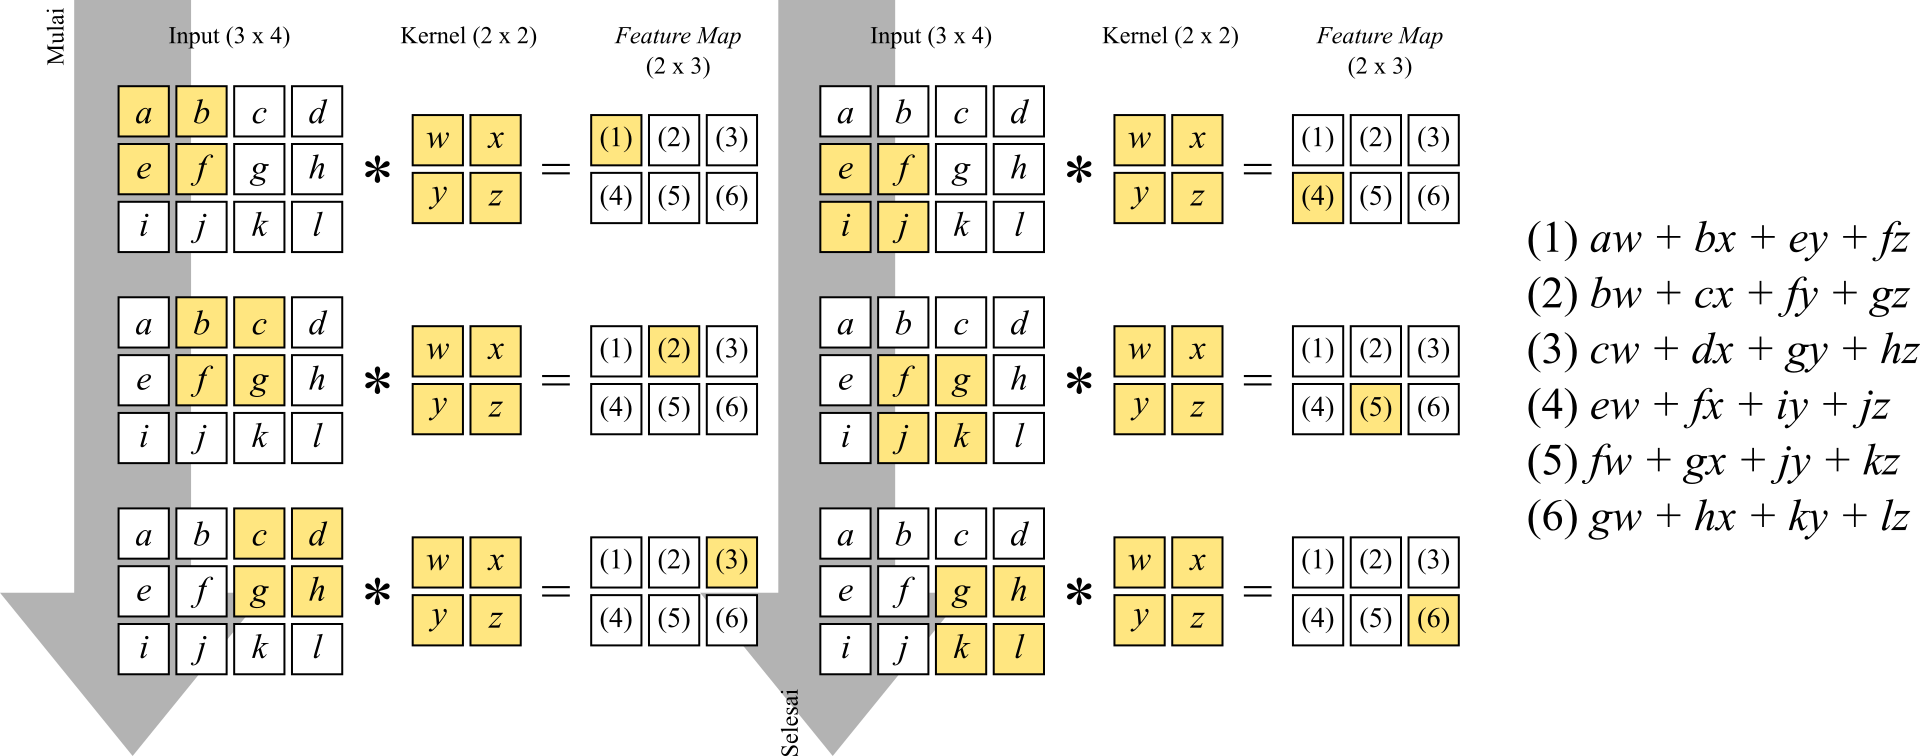
\includegraphics[width=14cm]{gambar/contoh_konvolusi1.png}
        \caption{\footnotesize Konvolusi \acrshort{2d} oleh Kernel $2 \times 2$ dengan \textit{Stride} $1 \times 1$ tanpa \textit{Zero Padding}}
        \label{fig:konvolusi1}
    \end{subfigure}
    \begin{subfigure}[t]{14cm}
        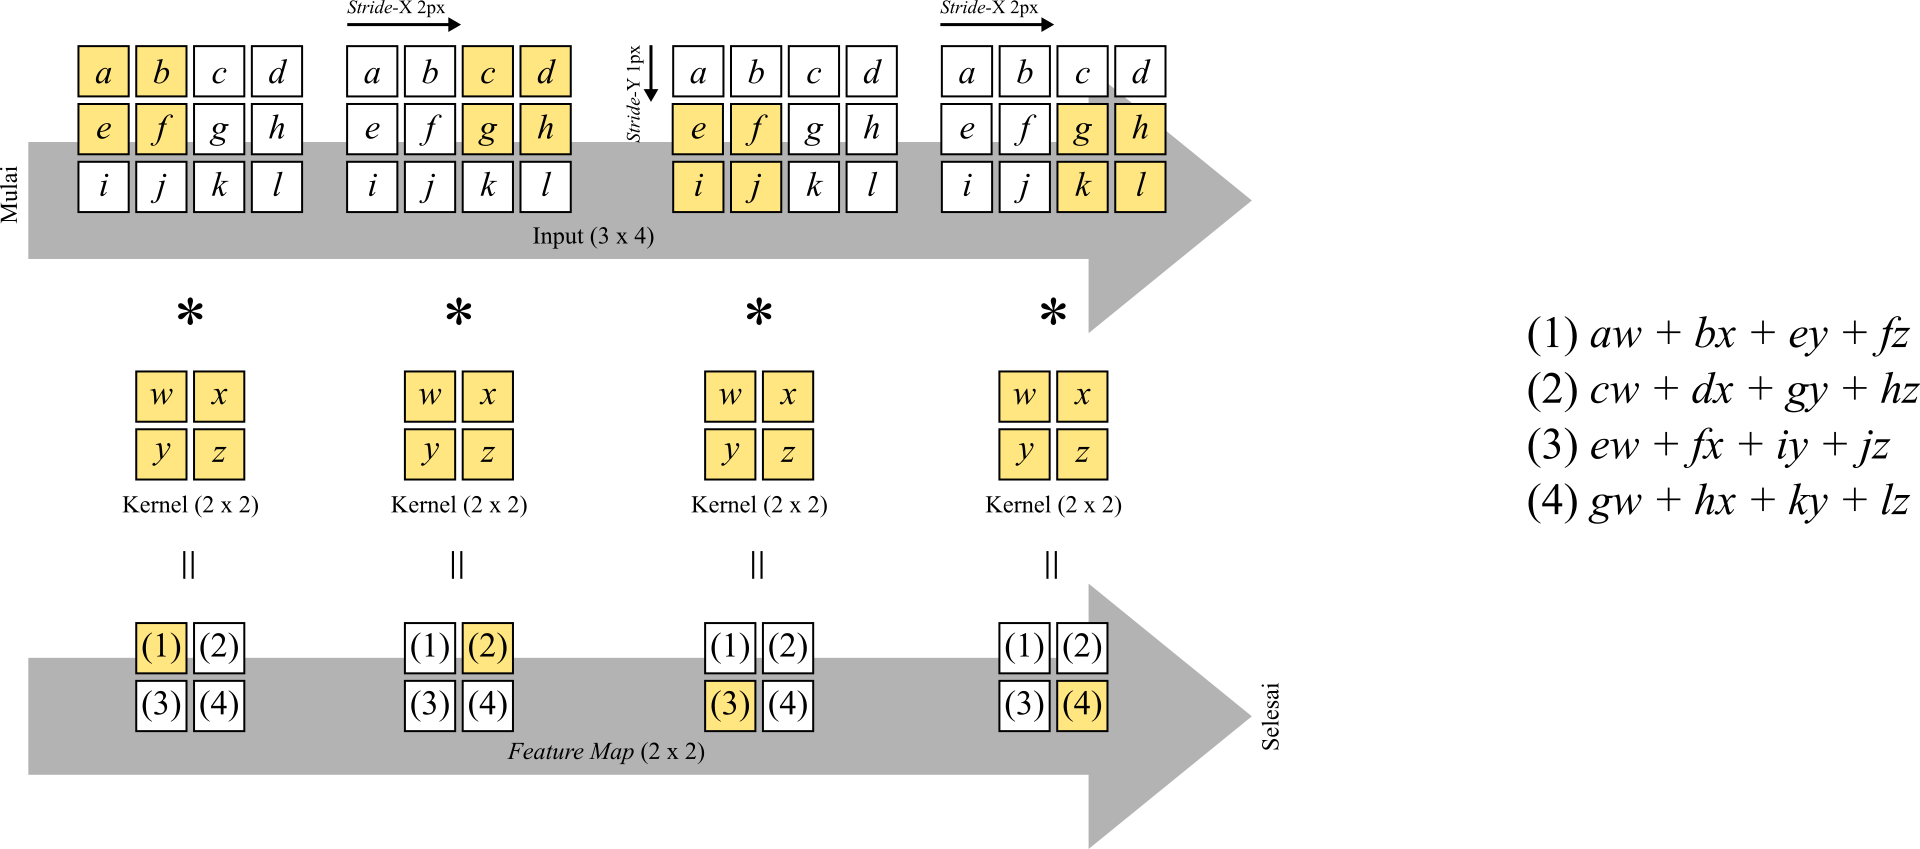
\includegraphics[width=14cm]{gambar/contoh_konvolusi2.png}
        \caption{\footnotesize Konvolusi \acrshort{2d} oleh Kernel $2 \times 2$ dengan \textit{Stride} $2 \times 1$ tanpa \textit{Zero Padding}}
        \label{fig:konvolusi2}
    \end{subfigure}
    \begin{subfigure}[t]{14cm}
        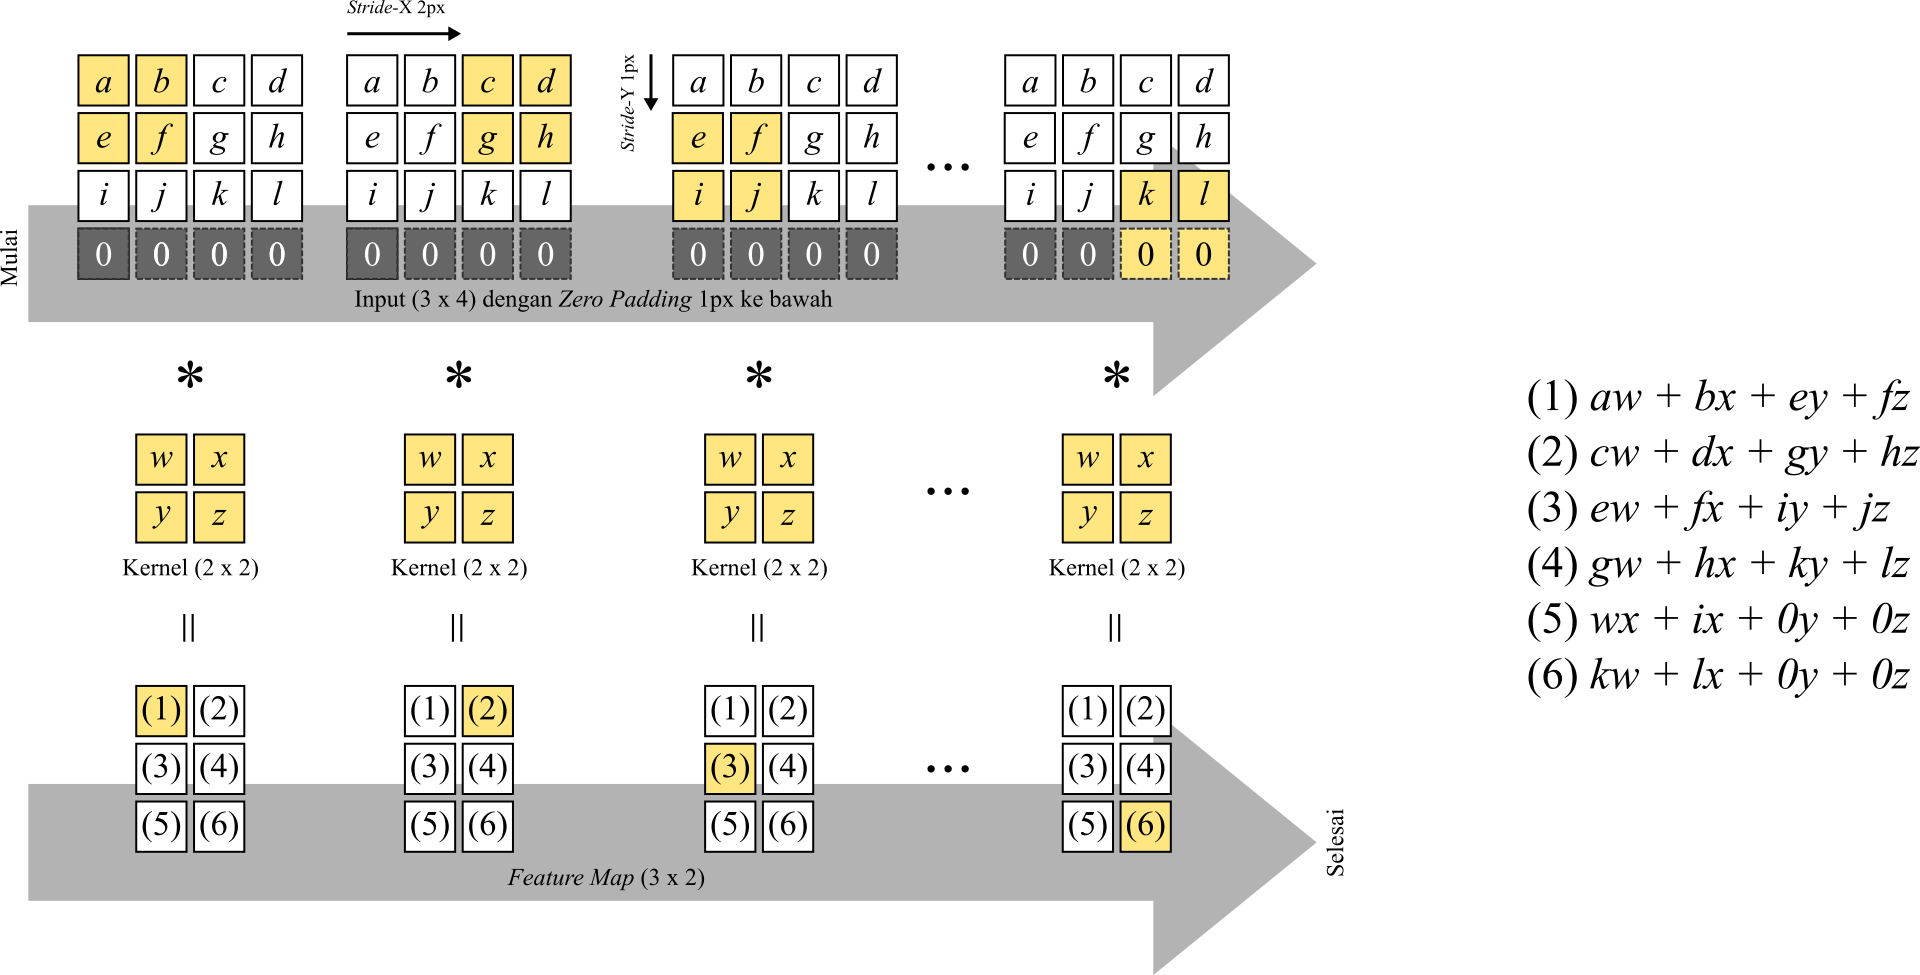
\includegraphics[width=14cm]{gambar/contoh_konvolusi3.png}
        \caption{\footnotesize Konvolusi \acrshort{2d} oleh Kernel $2 \times 2$ dengan \textit{Stride} $2 \times 1$ dan \textit{Zero Padding}}
        \label{fig:konvolusi3}
    \end{subfigure}
    \caption[Kasus-Kasus Konvolusi \acrshort{2d}]{Kasus-Kasus Konvolusi \acrshort{2d} \protect\shortcite{goodfellow2016deep}}
    \label{fig:contoh_konvolusi}
\end{figure}
Gambar \ref{fig:konvolusi1} memperlihatkan contoh konvolusi input $I(3,4)$ oleh kernel $K(2,2)$ menghasilkan \textit{feature map} $F(2,3)$. \acrshort{cnn} biasanya memiliki interaksi atau konektivitas \textit{sparse} ketika ukuran kernel lebih kecil daripada ukuran input. Tujuannya adalah mengurangi jumlah memori yang dibutuhkan untuk menyimpan parameter-parameter dari fitur-fitur gambar yang berarti. Jika ukuran kernel diperbesar, maka ukuran \textit{feature map} akan lebih kecil. Dan begitu pula sebaliknya. Di lapangan, konvolusi memiliki parameter tambahan yang disebut sebagai \textit{stride}, yang mana parameter ini mengatur seberapa besar pergeseran operasi perkalian oleh kernel terhadap input. \textit{Stride} yang berukuran lebih besar akan menghasilkan \textit{feature map} yang lebih kecil. Gambar \ref{fig:konvolusi2} menunjukkan bagaimana ukuran \textit{stride} yang berbeda, dari contoh pada Gambar \ref{fig:konvolusi1}, dapat mempengaruhi pemetaan dari input ke \textit{feature map} melalui proses konvolusi. Pemetaan dari input ke \textit{feature map} tanpa penambahan apapun terhadap input sering disebut sebagai konvolusi yang valid. Kita juga dapat mengendarai ukuran \textit{feature map} dengan melakukan zero padding pada input, di mana input diperluas dengan menambahkan aksis tertentu yang semua pikselnya bernilai nol seperti yang ditunjukkan pada Gambar \ref{fig:konvolusi3} \shortcite{goodfellow2016deep}.

Praproses data merupakan tahap yang cukup penting untuk pemodelan klasifikasi gambar. Praproses harus dilakukan secara hati-hati melalui analisis karakteristik data inputan. Pemilihan praproses yang tepat menghasilkan tahap ekstraksi fitur yang lebih baik. Sebaliknya, pemilihan yang tidak tepat dapat merusak atau bahkan menghilangkan fitur. Beragam praproses telah diterapkan oleh penelitian-penelitian terkait terdahulu, di antaranya adalah \textit{data augmentation}, \textit{illumination normalization}, \textit{face alignment} dan \textit{pose normalization}.

% TODO: histogram equalization

\textit{\acrlong{zca}} (\acrshort{zca}) merupakan teknik \textit{image whitening} yang terbukti mengungguli performa model klasifikasi gambar yang dikenakan oleh teknik normalisasi rerata dan standarisasi piksel gambar. Beberapa contoh hasil penggunaan teknik ini ditunjukkan pada Gambar \ref{fig:contohhasilzca}. Sementara fungsi \acrshort{zca} \shortcite{pal2016preprocessing} dijelaskan pada (\ref{equ:zca}),
\begin{equation}
    X_{\text{ZCA}} = U.\text{diag}(1/\sqrt{\text{diag}(S)+\epsilon}).U^T.X'
    \label{equ:zca}
\end{equation}
\begin{equation}
    X' = X/255
    \label{equ:normalisasi}
\end{equation}
dimana,
\begin{description}[align=parleft,labelwidth=2cm]
    \item[$U$] $= \parbox[t]{10.3cm}{matriks vektor Eigen,}$
    \item[$U^T$] $= \parbox[t]{10.3cm}{matriks transpos dari $U$,}$
    \item[diag($M$)] $= \parbox[t]{10.3cm}{diagonal matriks $M$,}$
    \item[$S$] $= \parbox[t]{10.3cm}{matriks nilai Eigen dari dekomposisi nilai singular matriks \textit{covariance},}$
    \item[$\epsilon$] $= \parbox[t]{10.3cm}{koefisien \textit{whitening},}$
    \item[$X'$] $= \parbox[t]{10.3cm}{hasil normalisasi oleh penskalaan fitur terhadap data $X$.}$
\end{description}
\begin{figure}[t]
    \centering
    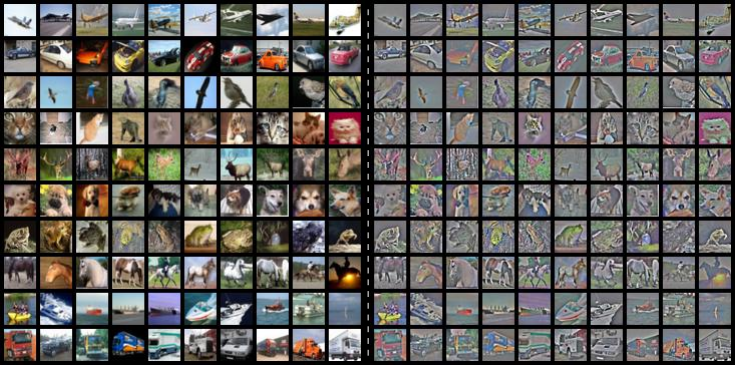
\includegraphics[width=14cm]{gambar/contoh_zca.png}
    \caption[Contoh-Contoh Hasil \acrshort{zca}]{Contoh-Contoh Hasil \acrshort{zca} \protect\shortcite{pal2016preprocessing}}
    \label{fig:contohhasilzca}
\end{figure}

\begin{figure}[t]
    \centering
    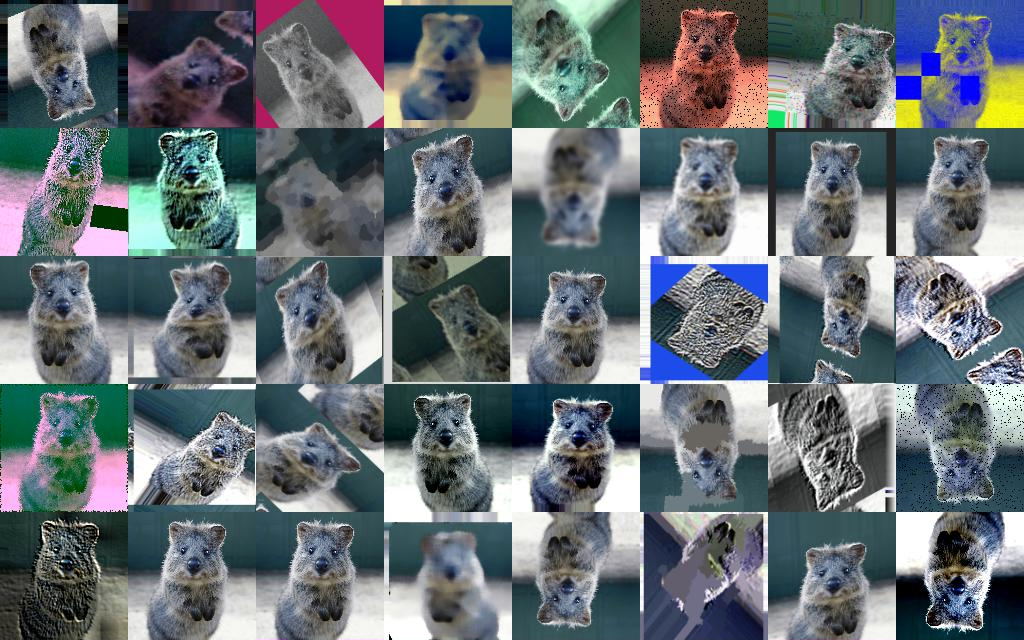
\includegraphics[width=14cm]{gambar/contoh_hasil_imgaug.png}
    \caption[Contoh-Contoh Hasil Augmentasi Data]{Contoh-Contoh Hasil Augmentasi Data (https://github.com/aleju/imgaug)}
    \label{fig:contohhasilimgaug}
\end{figure}

\begin{figure}[t]
    \centering
    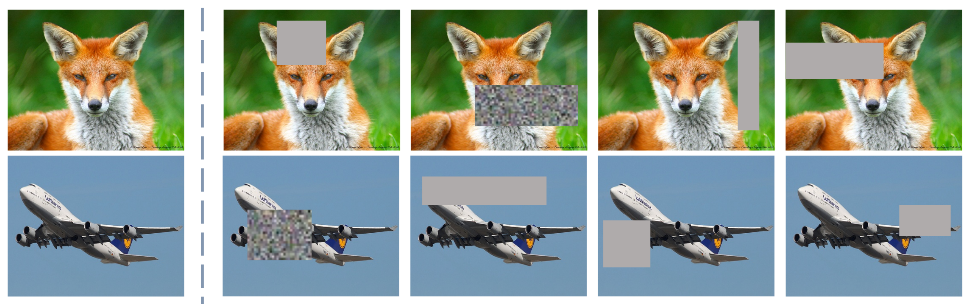
\includegraphics[width=14cm]{gambar/contoh_hasil_random_erasing.png}
    \caption[Contoh-Contoh Hasil Random Erasing]{Contoh-Contoh Hasil Random Erasing \protect\shortcite{zhong2017random}}
    \label{fig:contohrandomerasing}
\end{figure}

\textit{Data augmentation} biasa diterapkan untuk mengatasi \textit{overfitting} pada pelatihan model \acrshort{cnn} dengan set data yang terbatas. \textit{Data augmentation} dapat dilakukan baik menggunakan pendekatan konvensional (filter kernel, transformasi geometri, penghapusan acak, transformasi ruang warna dan pembauran gambar-gambar) maupun \textit{deep learning} (\textit{adversarial learning}, \textit{neural style transfer} dan GAN \textit{data augmentation}). \textit{Data augmentation} juga dapat dilakukan menggunakan \textit{meta learning}, yaitu paduan dari kedua pendekatan tersebut. Gambar \ref{fig:contohhasilimgaug} menunjukkan beberapa contoh hasil augmentasi data. Sejauh ini berdasarkan hasil eksperimen, pendekatan tradisional yang paling efektif dalam meningkatkan akurasi model adalah teknik \textit{cropping}, yaitu sebuah teknik pemrosesan gambar yang bekerja dengan menghilangkan sekumpulan piksel tertentu dari gambar \shortcite{shorten2019survey}. Di antara teknik \textit{cropping} yang paling populer dalam meningkatkan ketahanan model \acrshort{cnn} terhadap set data kecil adalah \textit{random erasing}, di mana teknik ini menghilangkan satu atau dua area piksel gambar secara acak (Gambar \ref{fig:contohrandomerasing}). Area-area gambar yang dihapus digantikan oleh piksel-piksel yang serupa atau sebarang \shortcite{zhong2017random,o2019comparing}. Penjelasan mendetail mengenai \textit{data augmentation} dapat dipelajari pada \shortciteA{shorten2019survey}.

\subsection{\textit{\acrlong{gcns}}}
\begin{figure}
    \centering
    \begin{subfigure}[t]{6.5cm}
        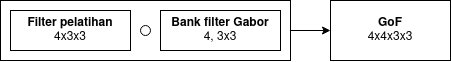
\includegraphics[width=6.5cm]{gambar/modulasi_gofs.png}
        \caption{Proses Modulasi \acrshort{gofs}}
        \label{fig:modulasigabor}
    \end{subfigure}
    ~~~
    \begin{subfigure}[t]{6.5cm}
        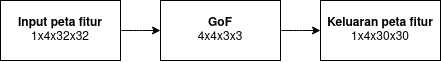
\includegraphics[width=6.5cm]{gambar/konvolusi_gofs.png}
        \caption{Contoh Konvolusi oleh \acrshort{gofs}}
        \label{fig:konvolusigofs}
    \end{subfigure}
    \caption[Modulasi dan Konvolusi \acrshort{gofs} di \acrshort{gcns}]{Modulasi dan Konvolusi \acrshort{gofs} di \acrshort{gcns} \protect\shortcite{luan2018gabor}}
    \label{fig:gofs}
\end{figure}
\begin{figure}[t]
    \centering
    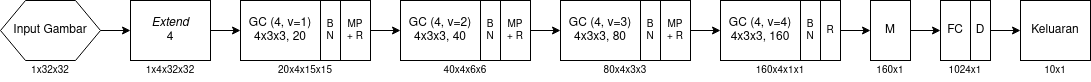
\includegraphics[width=14cm]{gambar/gcns.png}
    \caption*{\footnotesize{C---Konvolusi Spasial; MP---Max-Pooling; R---ReLu; M---Max; BN---BatchNormalization; D: Dropout}}
    \caption[Arsitektur \acrshort{gcns}]{Arsitektur \acrshort{gcns} \protect\shortcite{luan2018gabor}}
    \label{fig:gcns}
\end{figure}
\textit{\acrlong{gcns}} (\acrshort{gcns}), yang pertama kali diperkenalkan oleh \shortciteA{luan2018gabor}, merupakan \acrshort{dcnns} yang dimasuki oleh filter konvolusi \textit{\acrlong{gofs}} (\acrshort{gofs}) untuk meningkatkan ketahanan fitur yang dipelajari dalam perubahan skala dan orientasi. \acrshort{gofs} merupakan lapisan konvolusi dari modulasi filter pelatihan oleh filter Gabor dengan variasi skala dan orientasi. Gambar \ref{fig:gofs} menunjukkan bagaimana proses modulasi \acrshort{gofs} berlangsung. Sedangkan Gambar \ref{fig:gcns} menunjukkan bagaimana \acrshort{gofs} menempati setiap lapisan konvolusi pada jaringan tersebut.

\section{\textit{\acrlong{frs}}}
Pada studi segmentasi bagian wajah dalam konteks pengenalan ekspresi, tidak ada kesepakatan tentang bagaimana segmentasi yang optimal itu. Namun berdasarkan studi literatur, penulis menyimpulkan bahwa mayoritas penelitian menggunakan tiga bagian wajah yang paling menonjol pada pengenalan emosi. Ketiga bagian tersebut secara berurutan adalah mata, hidung, dan mulut \shortcite{guo2012holistic}. Proporsi kontribusi ketiga bagian tersebut hampir sama untuk setiap emosi \textit{angry}, \textit{disgust}, \textit{fear}, \textit{happy}, \textit{sad}, \textit{surprise}, dan \textit{neutral}. \shortciteA{benitez2018multicultural} membuktikan bahwa pengenalan ekspresi dengan tiga bagian ini mengungguli pengenalan menggunakan empat bagian, yaitu mata, hidung, mulut, dan dahi.

Segmentasi bagian wajah dapat dilakukan melalui berbagai cara, di antaranya melalui pendekatan \textit{grid/block based} dan \textit{local region based}. Dalam penelitian tersebut, mereka membagi wajah menjadi delapan belas bagian (Gambar \ref{fig:segmentasi18}) di mana area mata dibagi menjadi enam bagian, area hidung dibagi menjadi dua bagian dan sepuluh bagian sisanya untuk dahi, pipi dan dagu. Segmentasi area mulut pun dibuat sangat spesifik dengan membaginya berdasarkan garis luar bibir. Hasil eksperimen menunjukkan bahwa representasi \textit{local region based} lebih baik daripada representasi holistik dalam \textit{face registration} \shortcite{ghimire2015facial}. Ini menunjukkan bahwa mendefinisikan \acrshort{roi} secara spesifik dapat meningkatkan kualitas ekstraksi fitur.

% TODO: pustaka opencv (scaling, histogram equalization), FAN/RetinaFace (face detection + facial landmark detection), LogGabor dll.

\chapter{Metode Penelitian}

\section{Perancangan Penelitian}

\dots

\subsection{Perumusan Masalah}

\dots

\subsection{Studi Literatur}

\dots

\subsection{Pengumpulan Data}

\dots

\subsection{Perancangan Metode}

\dots

\subsection{Pengembangan Metode}

\dots

\subsection{Evaluasi Metode}

\dots

\section{Alat dan Bahan Penelitian}

\dots

\chapter{Temuan dan Pembahasan}
Pada bab ini disajikan berbagai temuan dan pembahasan secara komprehensif terhadap tahap-tahap pelaksanaan eksperimen dan pengujian yang berhasil dilakukan pada setiap skenario yang telah dirancang.

\section{\textit{Data Cleansing}}
Set data FER-2013 didistribusikan resmi dalam sebuah \textit{file} teks CSV\footnote{CSV atau \textit{Comma-Separated Value}, merupakan format \textit{file} teks khusus berbentuk tabel di mana setiap nilai dipisahkan menggunakan tanda koma.} berukuran 301,1MB. Sementara itu, pemuatan \textit{file} menggunakan pustaka \textit{pandas} hanya memerlukan memori sebesar 291,2MB. \textit{File} tersebut terdiri dari 35.887 baris dan 3 kolom, yaitu \textit{emotion}, \textit{pixels} dan \textit{Usage}. Setiap kolom berturut-turut memuat 7 label emosi dalam rentang nilai integer 0--6 (0: \textit{angry}, 1: \textit{disgust}, 2: \textit{fear}, 3: \textit{happy}, 4: \textit{sad}, 5: \textit{surprise} dan 6: \textit{neutral}), 2.304 piksel gambar dalam rentang nilai 0--255 dan 3 jenis penggunaan yang unik (\textit{Training}: set data \textit{training}, \textit{PrivateTest}: set data \textit{validation} dan \textit{PublicTest}: set data \textit{testing}). Adapun distribusi data telah dijelaskan pada bab yang sebelumnya.

Berdasarkan pengecekan secara hati-hati dan menyeluruh, setiap entri data adalah unik. Sehingga dapat dipastikan bahwa tidak ada irisan entri data yang sama untuk penggunaan yang berbeda. Meskipun dalam pemeriksaan singkat, ditemukan beberapa gambar yang terlihat sangat mirip. Namun hal ini tidak akan menjadi masalah, sebab tidak ada data gambar yang memiliki piksel-piksel yang tepat sama.

\textit{Data cleansing} dimulai dengan pemeriksaan data rusak, tidak relevan atau tidak lengkap. Pemeriksaan khusus data gambar dilakukan secara manual satu per satu supaya menyeluruh dan akurat. Alhasil disimpulkan bahwa setiap entri data adalah lengkap. Sayangnya, sejumlah data gambar sebanyak kurang lebih 85 buah ditemukan rusak, yaitu data gambar ke-59, 2059, 2171, 2809, 3262, 3931, 4275, 5082, 5274, 5439, 5722, 5881, 6102, 6458, 6699, 7172, 7496, 7527, 7629, 8030, 8737, 8856, 9026, 9500, 9673, 9679, 10423, 11244, 11286, 11295, 11846, 12289, 12352, 13402, 13697, 13988, 14279, 15144, 15553, 15838, 15894, 17081, 19238, 19632, 20222, 20712, 20817, 21817, 22198, 22314, 22407, 22927, 23596, 23894, 24053, 24441, 24891, 25219, 25603, 25909, 26383, 26860, 26897, 28601, 29447, 29557, 30002, 30705, 30981, 31127, 31825, 32662, 32683, 34334, 35121, 35469, 35632, 35743, 5509, 10023, 11826, 17620, 10219, 14550, dan 15389. Sehingga setiap entri data terkait perlu dihapus. Pada Gambar \ref{fig:contohdatagambarrusak}, ditampilkan beberapa contoh data gambar yang rusak. Yang banyak terlihat di sana adalah gambar sudah tidak dapat diakses kembali dari alamat web semula. Namun, yang membingungkan adalah semua itu masih merupakan \textit{file} gambar, yang mana seolah-olah gambar-gambar tersebut berupa hasil tangkapan layar (\textit{screenshot}).
\begin{figure}[t]
    \centering
    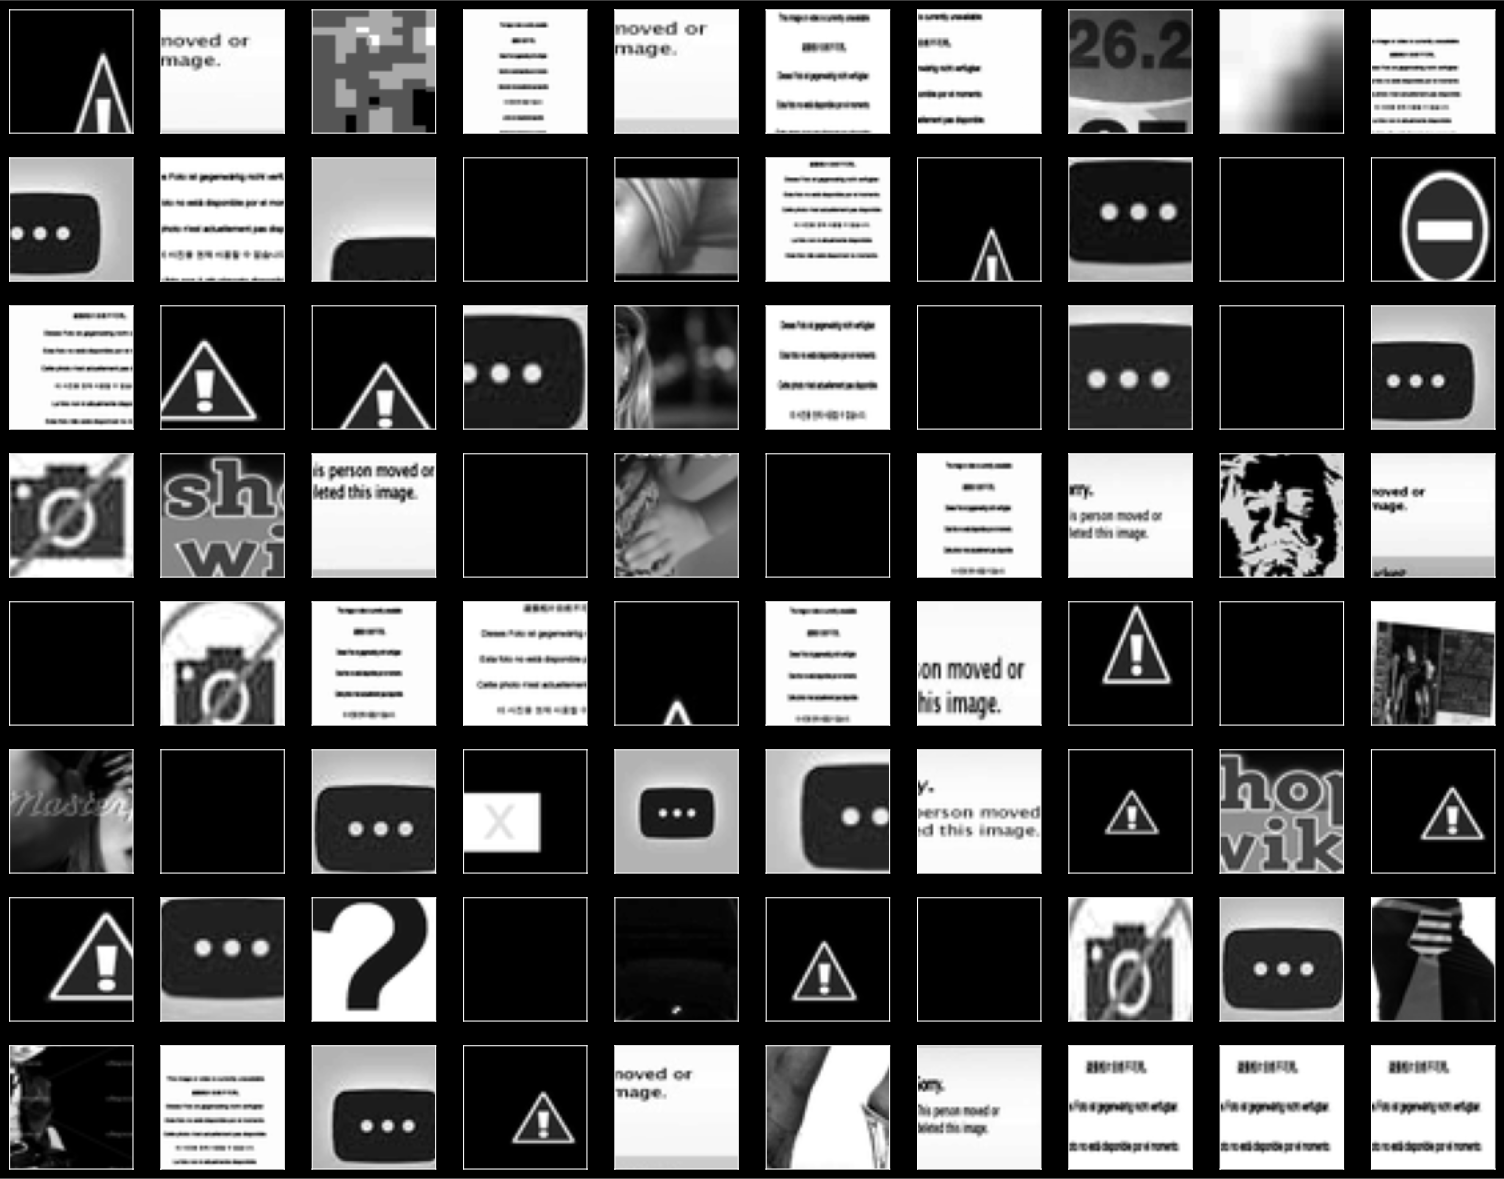
\includegraphics[width=14cm]{gambar/fer2013_data_rusak.png}
    \caption{Beberapa Contoh Data Gambar Rusak pada FER-2013}
    \label{fig:contohdatagambarrusak}
\end{figure}

\section{Praproses Data}
Pada skenario pertama, praproses data diawali dengan memperbesar (\textit{upscaling}) dimensi seluruh data gambar dari 48 $\times$ 48 piksel menjadi 64 $\times$ 64 piksel menggunakan \textit{opencv-python} dalam rangka penyesuaian ukuran set data gambar dengan dimensi lapisan input arsitektur model \acrshort{cnn} \textit{baseline}. %Beberapa contoh hasil proses ini dapat dilihat pada Gambar \ref{fig:contohupscaling}, di mana menghasilkan gambar yang tampak lebih halus meskipun tanpa interpolasi.
Selanjutnya, penulis mencoba menemukan teknik \textit{image enchancement} yang paling cocok untuk meningkatkan kualitas atau keterbacaan tiap-tiap gambar. Teknik-teknik yang akan penulis uji coba hanya berkisar pada teknik \textit{illumination normalization}. Namun, sebelum menerapkan teknik-teknik tersebut, penulis mengambil beberapa sampel gambar yang memiliki karakteristik yang cukup jauh. Dengan harapan bahwa sejumlah gambar tersebut dapat mewakili setiap variasi karakteristik gambar yang akan dikenakan teknik \textit{enhancement}.
% \begin{figure}[t]
%     \centering
%     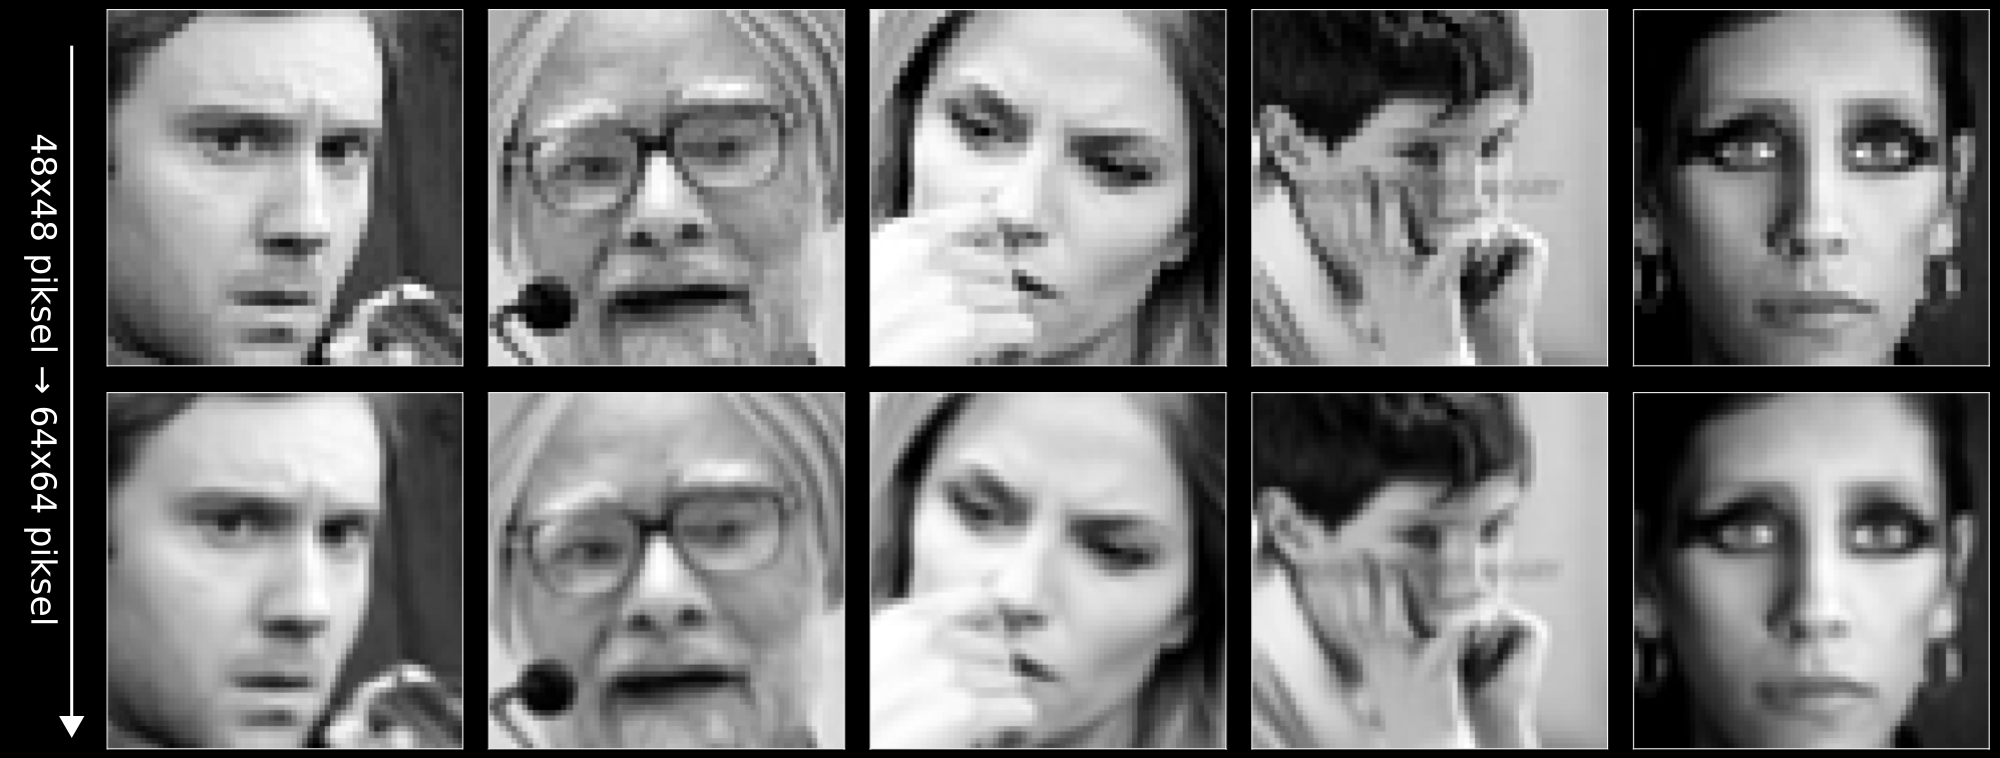
\includegraphics[width=14cm]{gambar/fer2013_contoh_upscaling.png}
%     \caption{Beberapa Contoh Hasil Proses \textit{Upscaling} terhadap FER-2013 dalam Ukuran yang Diseragamkan}
%     \label{fig:contohupscaling}
% \end{figure}

\begin{figure}
    \centering
    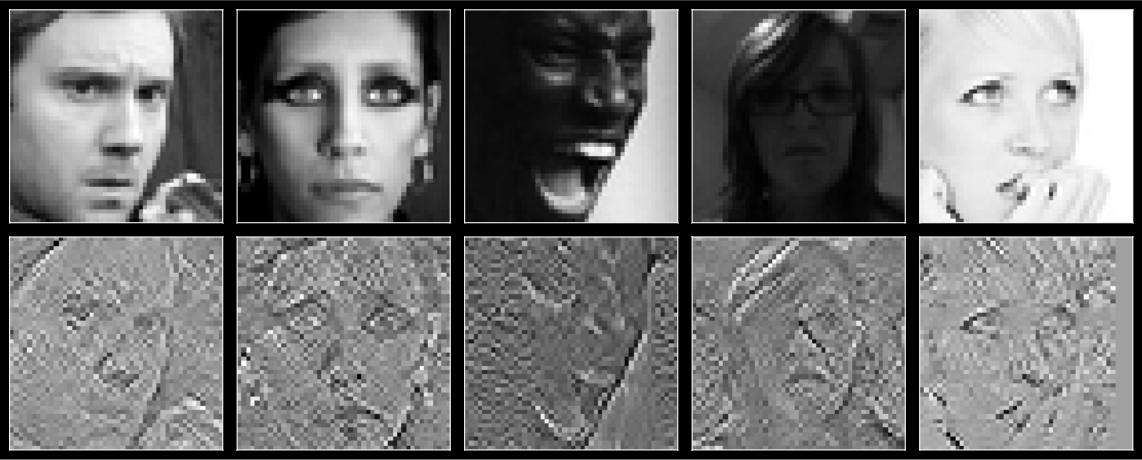
\includegraphics[width=14cm]{gambar/contoh_zca2.png}
    \caption{Beberapa Contoh Hasil Implementasi \acrshort{zca} terhadap FER-2013}
    \label{fig:contohzca2}
\end{figure}
Teknik pertama adalah \textit{image whitening} menggunakan \acrshort{zca} untuk menggantikan proses normalisasi yang disebutkan pada penelitian \textit{baseline}. Kode programnya diambil dari https://github.com/mwv/zca. Sayangnya, sebagaimana yang ditunjukkan pada Gambar \ref{fig:contohzca2}, pengenaan teknik ini ternyata menghilangkan banyak sekali informasi spasial mencakup informasi tekstur (seperti kerutan kulit di dahi dan pipi) dan garis tepi. Penulis menduga hal ini disebabkan oleh kecilnya resolusi gambar serta adanya limitasi dari \textit{grayscale}. Kekurangan ini tentunya sangat bertentangan dengan alasan mengapa penulis mengadopsi filter Gabor pada metode penelitian penulis.

\begin{figure}[t]
    \centering
    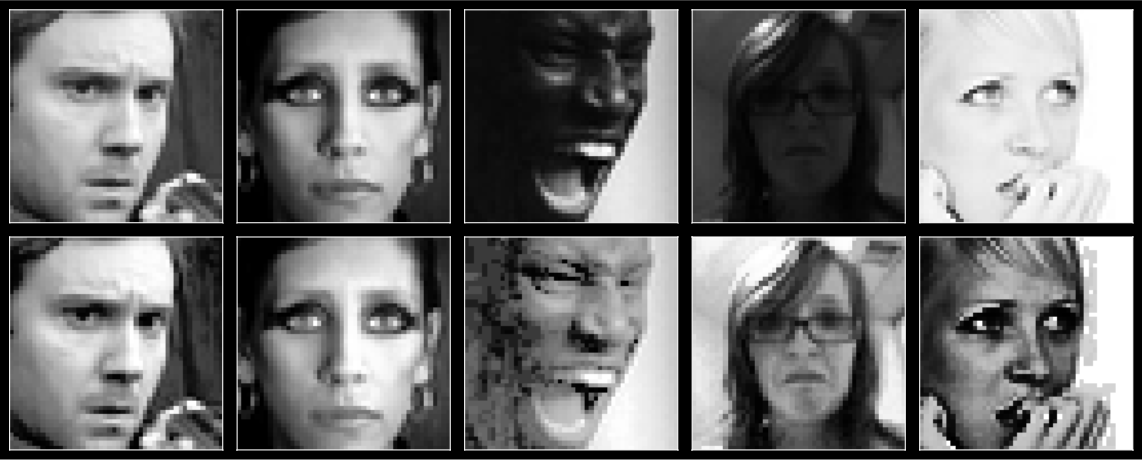
\includegraphics[width=14cm]{gambar/contoh_histogram_equalization.png}
    \caption{Beberapa Contoh Hasil Implementasi \textit{Histogram Equalization} terhadap FER-2013}
    \label{fig:contohhistogramequalization}
\end{figure}
Teknik kedua adalah \textit{histogram equalization} yang cukup populer dan dapat dipercaya terutama untuk meningkatkan kualitas area gambar yang relatif terlalu gelap. Hasilnya dapat dilihat pada Gambar \ref{fig:contohhistogramequalization}. Secara keseluruhan, teknik ini sangat andal dalam meningkatkan kualitas gambar baik yang terlalu gelap maupun terlalu terang. Namun, teknik ini gagal terhadap gambar yang memiliki kontras yang cukup jauh antara objek dan latar. Alhasil, kedua teknik ini tidak akan penulis gunakan pada penelitian ini.

\begin{table}
    \caption[Perbandingan Teknik-Teknik \textit{Facial Landmark Detection}]{Perbandingan Teknik-Teknik Facial Landmark Detection}
    \label{tab:teknikfaciallandmarkdetection}
    \begin{tabular}{|C{3.5cm}|C{2cm}|C{2.1cm}|C{0.8cm}|C{2cm}|C{0.9cm}|}
        \hline
        Pustaka & \textit{Loss} (\%)$^\bigtriangledown$ & Waktu (s)$^\bigtriangledown$ & \textit{n}$^\bigtriangleup$ & \textit{Threshold} & GPU \\
        \hline\hline
        \textit{face\_alignment} (face\_detector=sfd) & \multirow{2}{*}{3,10} & \multirow{2}{*}{2.786} & \multirow{2}{*}{68} & \multirow{6}{*}{0,5} & \multirow{6}{*}{\ding{51}} \\
        \cline{1-4}
        \textit{RetinaFace} (net=mobilenet0.25) & \multirow{2}{*}{42,23} & \multirow{2}{*}{334} & \multirow{4}{*}{5} &  &  \\
        \hhline{*{3}{|-}|~|}
        \textit{RetinaFace} (net=resnet50) & \multirow{2}{*}{7,05} & \multirow{2}{*}{476} &  &  &  \\
        \hline
    \end{tabular}
    \footnotesize
    {\raggedright
    \textit{Loss}---persentase banyak data gambar yang tidak terdeteksi wajah; Waktu---waktu total eksekusi pendeteksian \emph {facial landmark} untuk seluruh data gambar; \textit{n}---banyak \textit{facial landmark} per wajah;\\
    $^\bigtriangleup$Lebih tinggi lebih baik; $^\bigtriangledown$Lebih rendah lebih baik.}
\end{table}
Pada skenario kedua, penulis menambahkan empat langkah ekstra tepat sebelum memasuki tahap \textit{upscaling}. Tahap pertama merupakan pendeteksian area wajah pada setiap gambar dengan batas ambang (\textit{threshold}) sama dengan 0,5. Setiap area wajah yang ditandai dan berhasil melewati \textit{threshold} akan diteruskan ke tahap berikutnya, yaitu pendeteksian atau prediksi \textit{facial landmark}. Kedua tahap ini dapat ditangani baik secara terpisah maupun tergabung oleh berbagai pustaka yang telah tersedia publik. Penulis telah mencoba beberapa di antaranya dan membandingkan metode mana yang paling kredibel untuk diimplementasikan pada set data wajah nonfrontal, FER-2013. Namun, di sini penulis hanya akan membahas hasil dari dua metode terbaik, yaitu \textit{\acrlong{fan}} (\acrshort{fan}) dalam pustaka \textit{face\_alignment} \shortcite{bulat2017far} dan \textit{RetinaFace} \shortcite{deng2019retinaface}.

Sebagaimana yang disimpulkan pada Tabel \ref{tab:teknikfaciallandmarkdetection}, metode \acrshort{fan} unggul dalam kecilnya persentase kehilangan data dan banyaknya \textit{facial landmark} yang mampu diprediksi. Kendati pun waktu eksekusinya sangat lama, hal ini tidak akan menjadi masalah yang penting. Sementara itu, metode \textit{RetinaFace} memiliki waktu eksekusi relatif cukup cepat, namun memiliki persentase kehilangan data yang relatif besar. Terutama metode \textit{RetinaFace} yang menggunakan arsitektur MobileNet0.25, metode \textit{RetinaFace} kurang bisa diandalkan. Akan tetapi, masih perlu validasi tiap-tiap metode dengan mengambil beberapa sampel hasil deteksi \textit{facial landmark}.

\begin{figure}
    \centering
    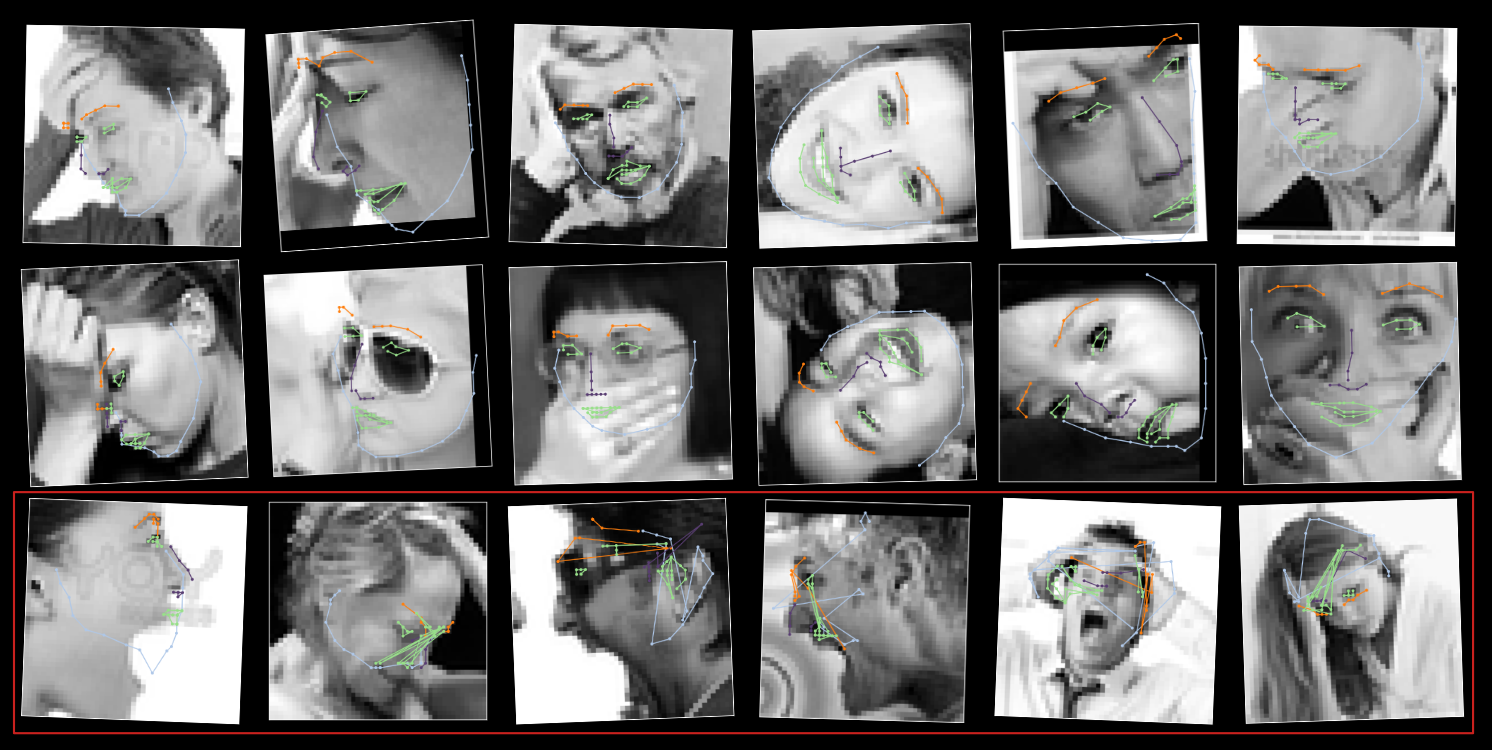
\includegraphics[width=14cm]{gambar/contoh_hasil_facealignment.png}
    \caption{Beberapa Contoh Hasil Deteksi \textit{Facial Landmark} terhadap FER-2013 Menggunakan \acrshort{fan}}
    \label{fig:contohhasilfacealignment}
\end{figure}
\begin{figure}
    \centering
    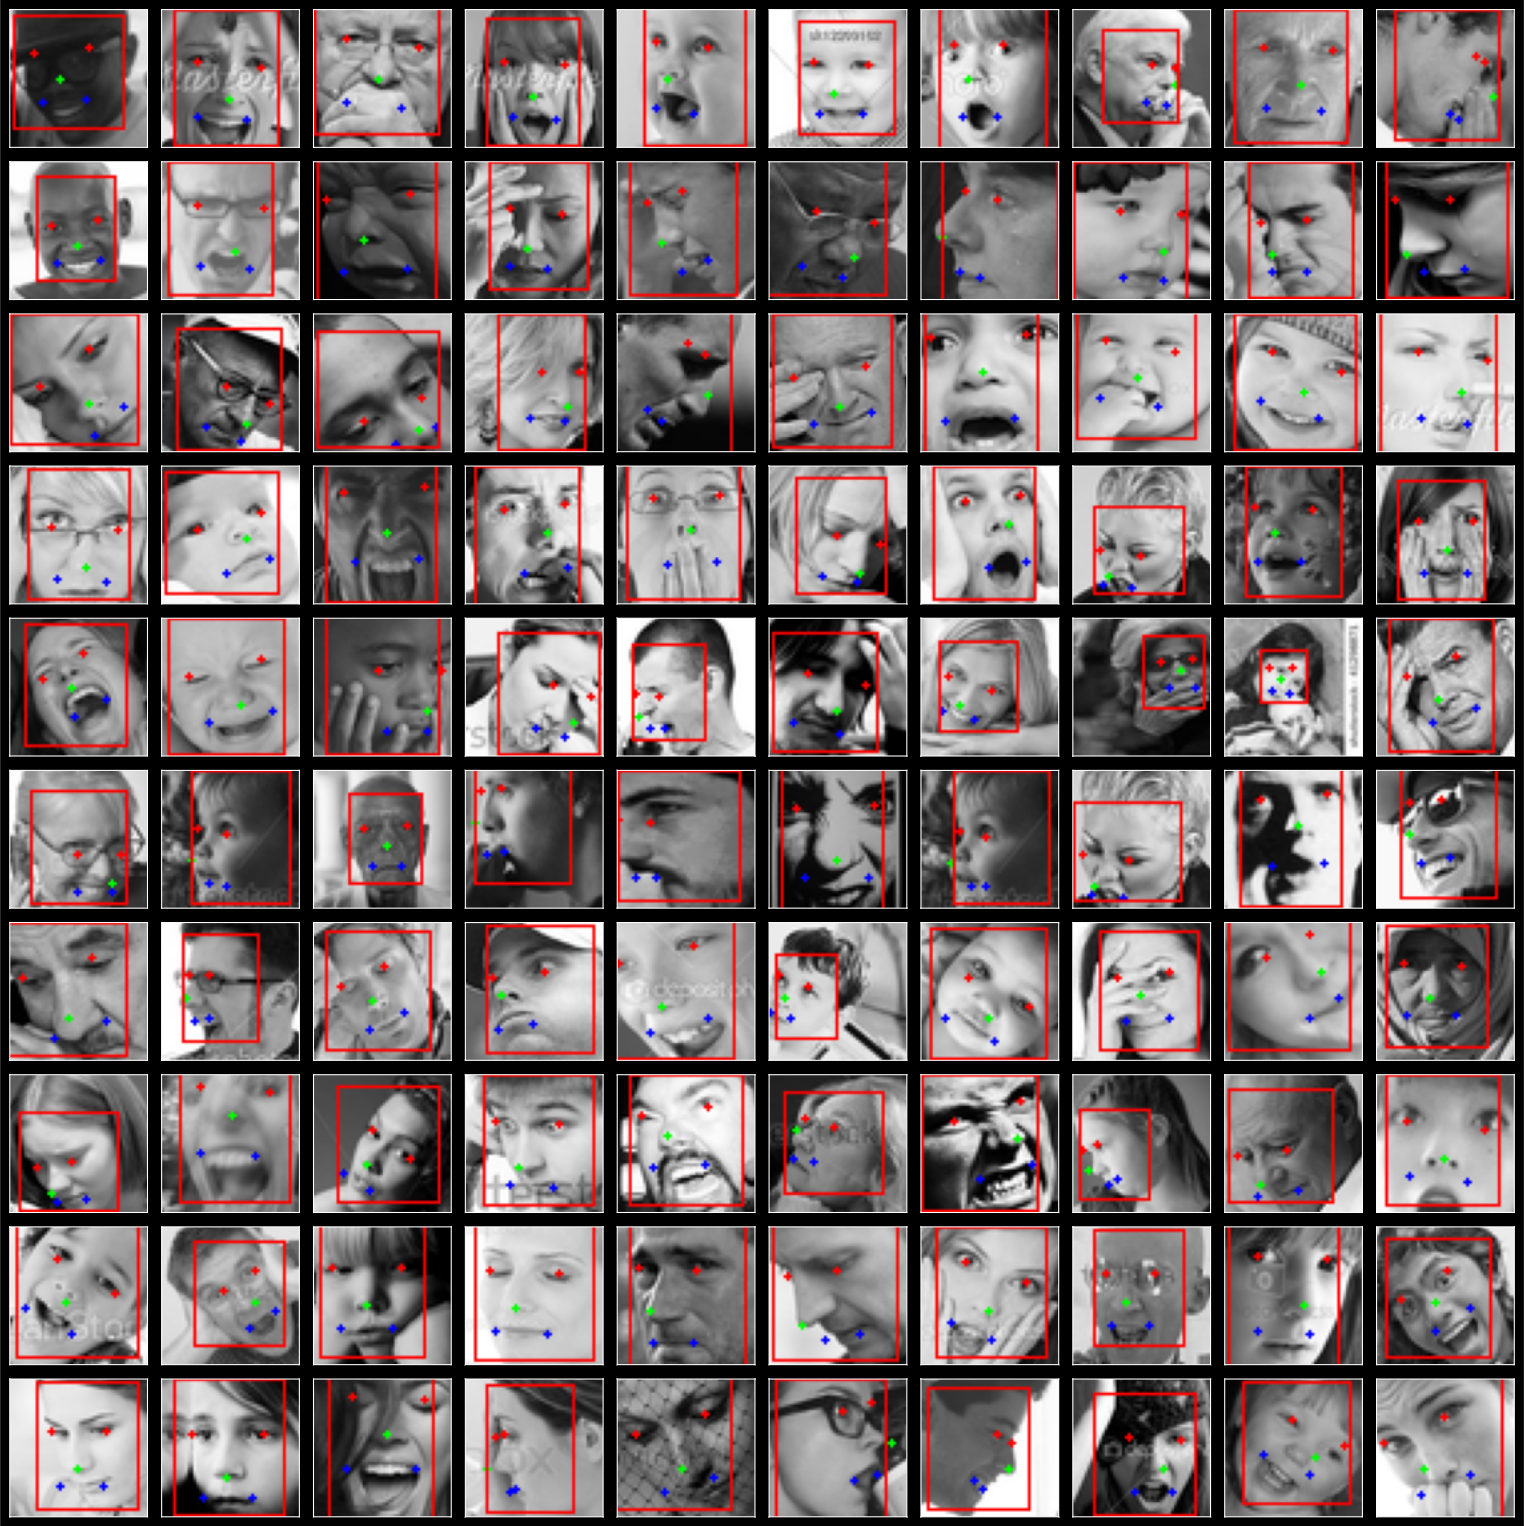
\includegraphics[width=14cm]{gambar/contoh_hasil_retinaface_score50.png}
    \caption{Beberapa Contoh Hasil Deteksi \textit{Facial Landmark} terhadap FER-2013 Menggunakan \textit{RetinaFace} pada ResNet50}
    \label{fig:contohhasilretinaface}
\end{figure}
Berdasarkan Gambar \ref{fig:contohhasilfacealignment} di baris pertama dan kedua, metode \acrshort{fan} sangat presisi dalam memprediksi \textit{facial landmark}. Bahkan berhasil memprediksi \textit{facial landmark} pada objek-objek wajah dengan rotasi yang sangat ekstrem dan/atau halangan yang cukup mengganggu. Namun, pendeteksiannya tidak akurat bahkan sangat berantakan untuk sampel gambar wajah di baris ketiga. Sayangnya, penulis pun tidak dapat menyimpulkan gambar-gambar wajah dengan karakteristik bagaimana yang gagal diprediksi. Oleh karena penulis kesulitan jika harus memeriksa satu per satu hasilnya, maka metode \acrshort{fan} dinilai tidak bisa diandalkan.

Kemudian penulis mencoba meninjau hasil prediksi metode \textit{RetinaFace} dengan ResNet50 yang ditunjukkan pada Gambar \ref{fig:contohhasilretinaface}. Di sini penulis mengambil sampel dari seratus gambar wajah pertama yang berhasil dikenali dan diprediksi dengan skor yang mendekati \textit{threshold}. Hasilnya, prediksi \textit{facial landmark} menggunakan metode ini cukup akurat dan presisi. Disertai kenyataan bahwa entri data terkait yang gagal dikenali tersebar cukup merata pada setiap label emosi, maka metode ini menjadi pilihan penulis yang terbaik dalam mendeteksi \textit{facial landmark}.

\begin{figure}
    \centering
    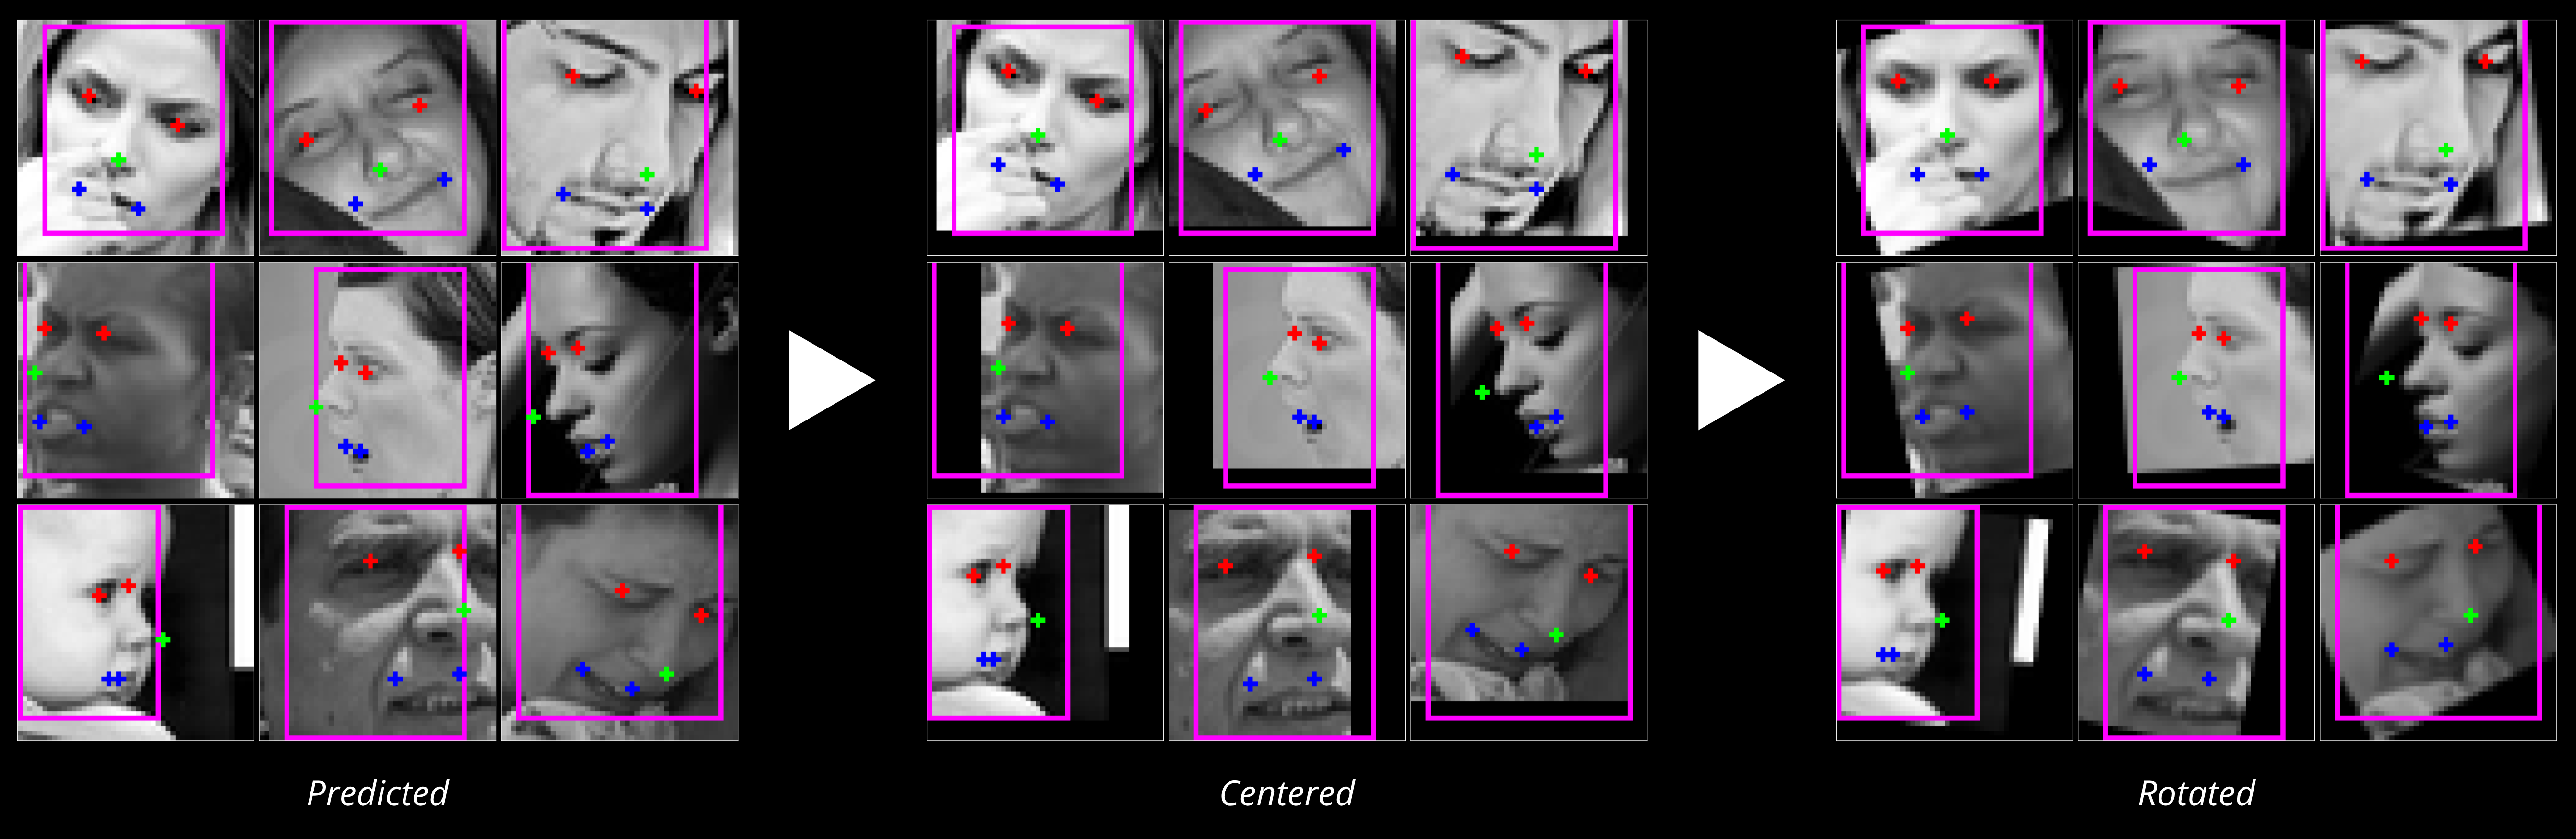
\includegraphics[width=14cm]{gambar/proses_face_alignment.png}
    \caption{Beberapa Contoh Hasil per Subtahap \textit{Face Alignment}}
    \label{fig:prosesfacealignment}
\end{figure}
Tahap ketiga adalah \textit{face alignment}, di mana dilakukan penjajaran setiap objek wajah menggunakan pustaka \textit{opencv} berdasarkan \textit{bounding box} wajah dan \textit{facial landmark} yang bersesuaian. Pertama-tama, sentralisasi setiap objek wajah dilakukan melalui penggeseran seluruh piksel gambar sejauh perpindahan antara titik senter semua \textit{facial landmark} ke titik senter \textit{bounding box} wajah. Lalu perotasian setiap objek wajah dilakukan terhadap titik senter \textit{bounding box} melalui teknik tertentu yang sesuai dengan salah satu dari tiga situasi yang telah didefinisikan. Situasi pertama adalah jika koordinat pada sumbu x tengara hidung berada di tengah-tengah antara tengara sisi kiri dan kanan bibir, maka perotasian dilakukan untuk menjajarkan koordinat pada sumbu y kedua tengara mata. Situasi kedua adalah jika koordinat pada sumbu x tengara hidung berada di kiri terhadap tengara sisi kiri bibir, maka perotasian dilakukan untuk menjajarkan koordinat pada sumbu x tengara mata kanan dan sisi kanan bibir. Situasi ketiga adalah jika koordinat pada sumbu x tengara hidung berada di kanan terhadap tengara sisi kanan bibir, maka perotasian dilakukan untuk menjajarkan koordinat pada sumbu x tengara mata kiri dan sisi kiri bibir. Setiap proses pada tahap ini direpresentasikan ke dalam Gambar \ref{fig:prosesfacealignment}, di mana setiap baris gambar mencontohkan hasil dari masing-masing situasi secara berurutan dari atas ke bawah.

\begin{figure}
    \centering
    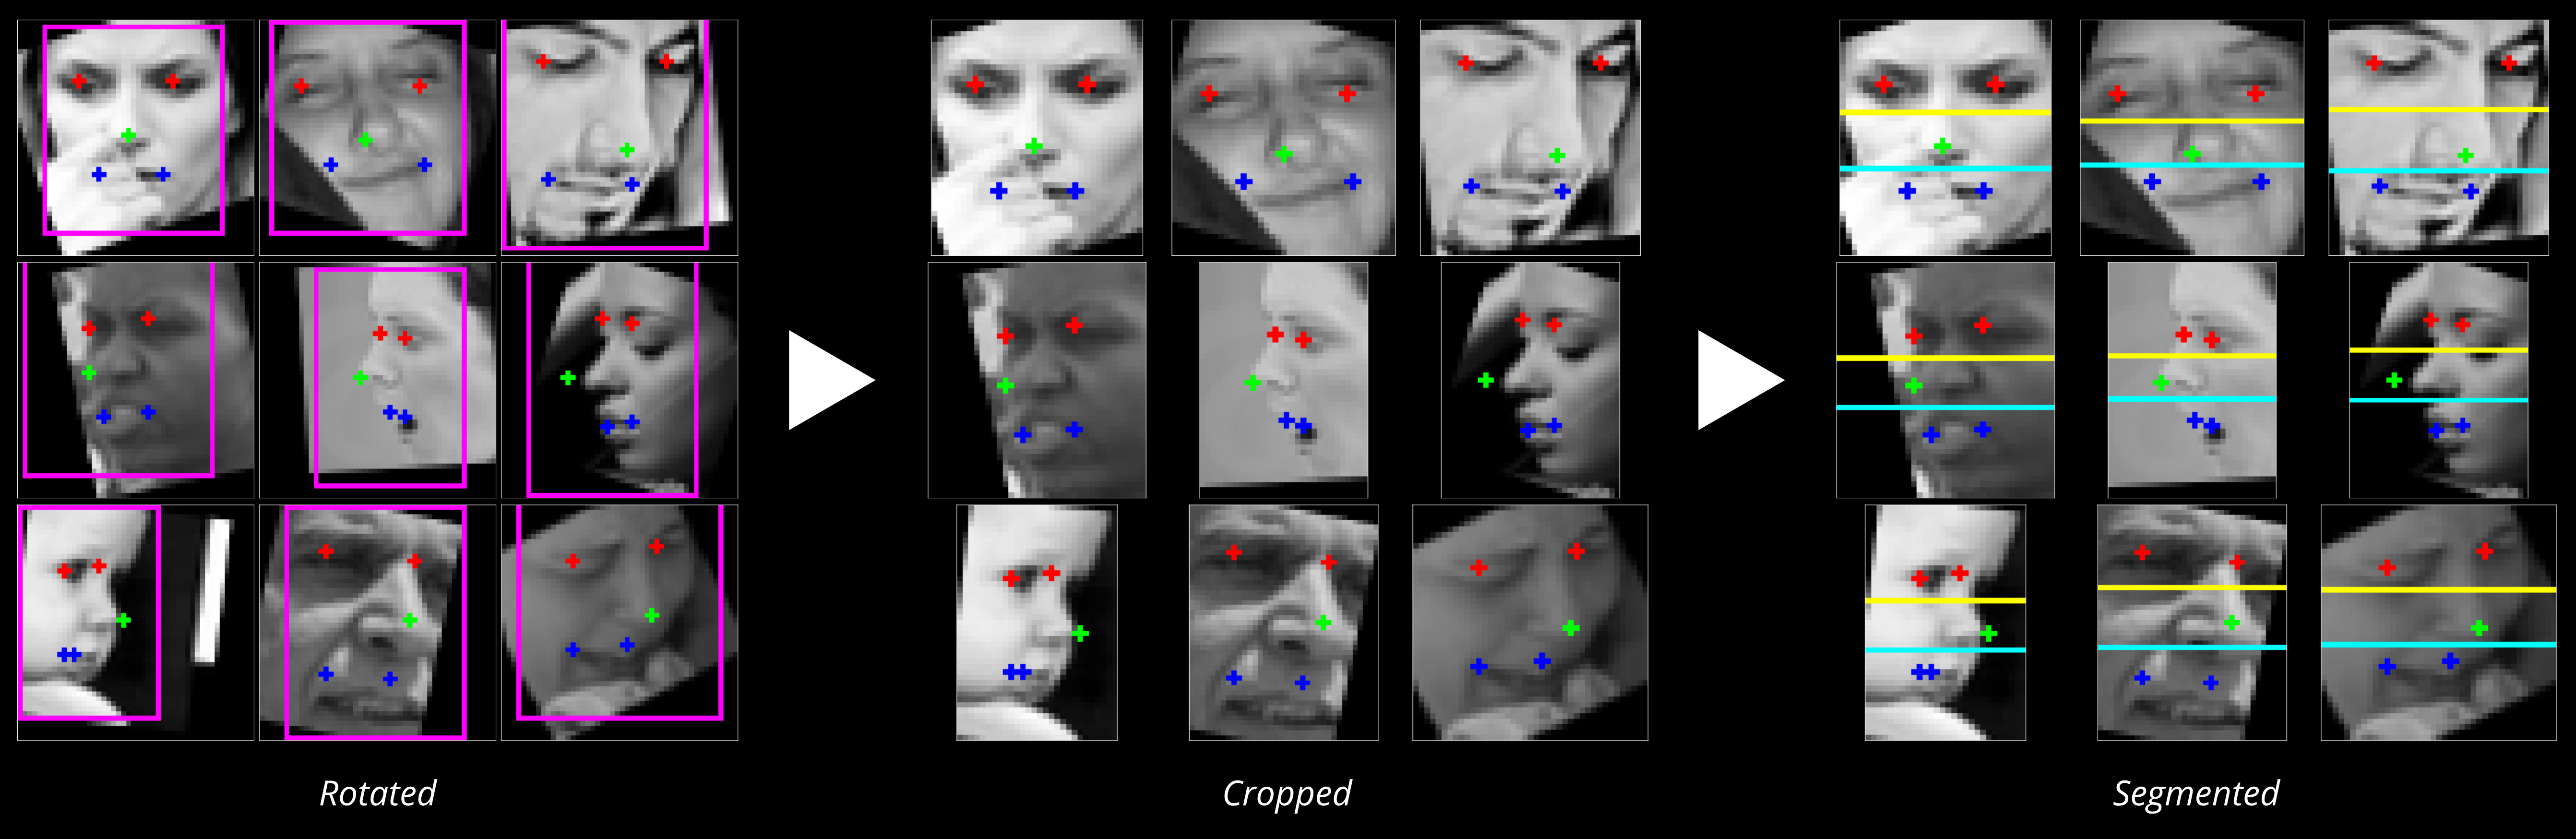
\includegraphics[width=14cm]{gambar/proses_facial_region_segmentation.png}
    \caption{Beberapa Contoh Hasil per Subtahap \textit{\acrlong{frs}}}
    \label{fig:prosesfacialregionsegmentation}
\end{figure}
Tahap keempat adalah \textit{facial region segmentation}, di mana tiap-tiap bagian wajah disegmentasi guna menghasilkan set data sekunder. Pada tahap ini, diusulkan dua konfigurasi segmentasi yang berbeda. Konfigurasi pertama adalah pembagian setiap objek wajah menjadi tiga area, yaitu kedua mata, hidung dan mulut. Sedangkan konfigurasi kedua adalah pembagian dua area yang saling tumpang tindih (\textit{overlapping}), yaitu area kedua mata hingga hidung dan area hidung hingga mulut. Proses segmentasi ini dilakukan dengan memotong gambar sesuai dengan \textit{bounding box}, melakukan kalkulasi ulang untuk tiap-tiap \textit{facial landmark} dan memotong gambar per area yang ditentukan. Setiap area yang dipotong didefinisikan oleh sisi-sisi \textit{bounding box} dan garis horizontal yang melalui titik tengah antar dua area yang bersinggungan. Misalnya untuk area kedua mata, dibatasi oleh sisi atas, kiri dan kanan \textit{bounding box} serta garis horizontal batas area kedua mata dan hidung. Contoh-contoh setiap proses pada tahap ini dapat dilihat pada Gambar \ref{fig:prosesfacialregionsegmentation}.

Secara khusus, melalui algoritma segmentasi yang dikembangkan pada penelitian ini, penulis berupaya menjawab permasalahan segmentasi bagian-bagian wajah pada set data wajah nonfrontal. Yang mana set data tersebut memuat berbagai variasi stuktur wajah yang berbeda \shortcite{islam2018facial3}.

\section{Eksekusi Skenario Pemodelan}
Pada subbab ini, penulis akan menjelaskan proses dan hasil eksperimen secara mendetail untuk setiap skenario pemodelan yang telah direncanakan. Setiap skenario dijalankan sebanyak tiga kali percobaan tanpa mengubah konfigurasi apapun untuk lalu diambil model dengan performa yang terbaik. Penggunaan statistik pada percobaan berulang merupakan solusi tradisional dalam menyimpulkan kinerja model. Meskipun pada dasarnya penulis telah mengeset \textit{seed} untuk setiap \textit{random number generator} ke nilai tertentu, performa model tetap terus berubah pada pengulangan percobaan yang berikutnya.

\subsection{Implementasi \acrshort{cnn} \textit{Baseline}}
\begin{table}[t]
    \caption[Perbandingan Performa Model \textit{Baseline} dengan dan tanpa Augmentasi Data]{Perbandingan Performa Model Baseline dengan dan tanpa Augmentasi Data}
    \label{tab:eksperimenbaseline}
    \begin{tabular}{|L{5.4cm}|C{2.6cm}|C{1.5cm}|C{2.7cm}|}
        \hline
        & Akurasi (\%)$^\bigtriangleup$ & \textit{Epoch} & Waktu (jam)$^\bigtriangledown$ \\
        \hline\hline
        Tanpa data augmentasi & 54,24 & 48 & 0,31 \\
        \hline
        Dengan data augmentasi & 60,27 & 174 & 1,64 \\
        \hline
    \end{tabular}
    \footnotesize
    {\raggedright Akurasi---akurasi model pada \textit{testing}; \textit{Epoch}---banyak \textit{epoch} yang dibutuhkan agar model menjadi optimal; Waktu---waktu yang dibutuhkan agar model menjadi optimal; $^\bigtriangleup$Lebih tinggi lebih baik; $^\bigtriangledown$Lebih rendah lebih baik.}
\end{table}
\begin{figure}[t]
    \centering
    \begin{subfigure}[t]{6.75cm}
        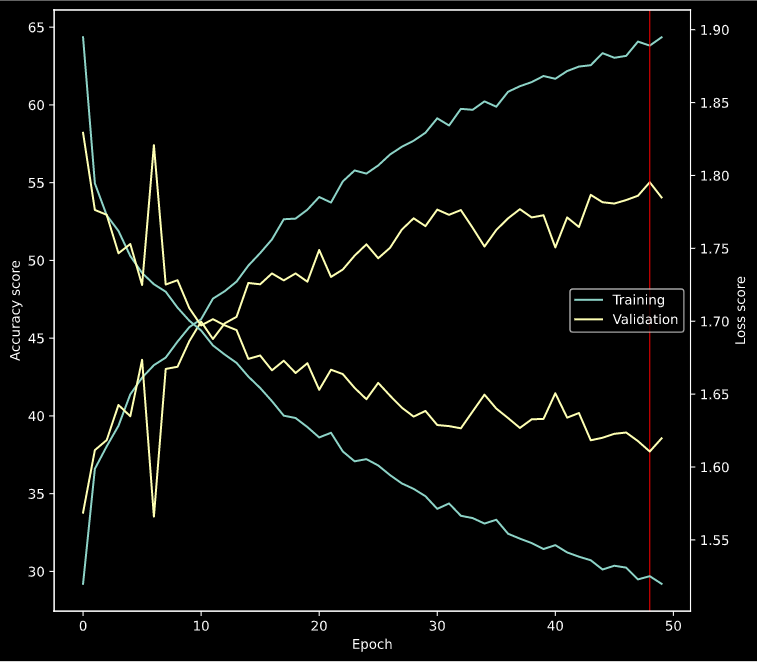
\includegraphics[width=6.75cm]{gambar/eksperimen1_grafik1.png}
        \caption{Grafik Performa Per \textit{Epoch} untuk Model tanpa Augmentasi Data}
        \label{fig:grafikeksperimen1}
    \end{subfigure}
    ~~~
    \begin{subfigure}[t]{6.75cm}
        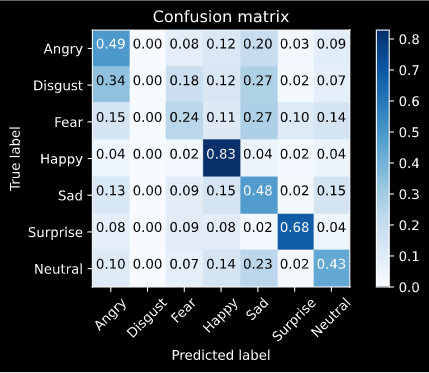
\includegraphics[width=6.75cm]{gambar/eksperimen1_matriks1.png}
        \caption{\textit{Confusion Matrix} Performa Model tanpa Augmentasi Data}
        \label{fig:confusionmatrixeksperimen1}
    \end{subfigure}
    \caption{Performa Model \acrshort{cnn} \textit{Baseline} tanpa Augmentasi Data}
    \label{fig:hasileksperimen1}
\end{figure}
\begin{figure}[!htb]
    \centering
    \begin{subfigure}[t]{6.75cm}
        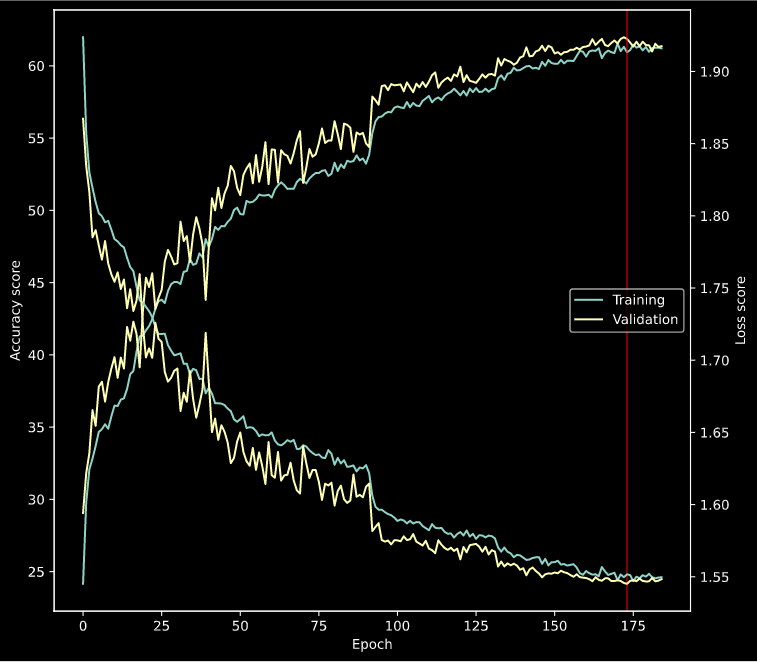
\includegraphics[width=6.75cm]{gambar/eksperimen2_grafik1.png}
        \caption{Grafik Performa Per \textit{Epoch} untuk Model dengan Augmentasi Data}
        \label{fig:grafikeksperimen2}
    \end{subfigure}
    ~~~
    \begin{subfigure}[t]{6.75cm}
        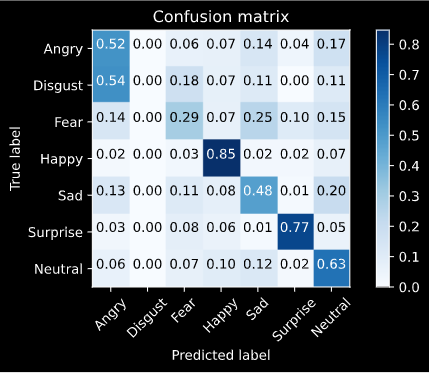
\includegraphics[width=6.75cm]{gambar/eksperimen2_matriks1.png}
        \caption{\textit{Confusion Matrix} Performa Model dengan Augmentasi Data}
        \label{fig:confusionmatrixeksperimen2}
    \end{subfigure}
    \caption{Performa Model \acrshort{cnn} \textit{Baseline} dengan Augmentasi Data}
    \label{fig:hasileksperimen2}
\end{figure}
\begin{figure}[t]
    \centering
    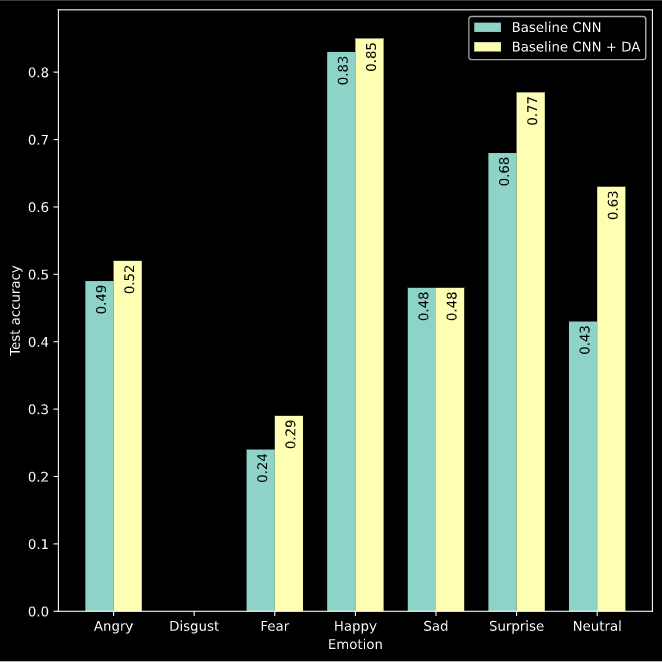
\includegraphics[width=10cm]{gambar/eksperimen1vs2_grafik1.png}
    \caption{Perbandingan Performa Model dengan dan\\tanpa Augmentasi Data Per Kelas Emosi}
    \label{fig:perbandinganeksperimen1dan2}
\end{figure}
Eksperimen dimulai dengan mengimplementasikan model \acrshort{cnn} \textit{baseline} pilihan untuk pengenalan ekspresi wajah pada set data FER-2013. Model yang diklaim dapat mencapai akurasi tes 65,23\% tersebut, berhasil penulis rekonstruksi ulang. Namun, penulis kesulitan bahkan hanya untuk mendekati akurasi tersebut. Penulis menduga terdapat beberapa alasan untuk hal ini. Pertama, yang mana merupakan hal yang paling penting, pembagian distribusi data \textit{training}, \textit{validation} dan \textit{testing} berbeda. Jika pada penelitian \textit{baseline} menggunakan rasio 80:20 untuk data \textit{training} dan \textit{testing}, penulis menggunakan rasio 80:10:10 berturut-turut untuk data \textit{training}, \textit{validation} dan \textit{testing} sesuai dengan \textit{default} dari set data FER-2013 sendiri. Dengan mempertimbangkan bahwa hampir seluruh penelitian pada FER-2013 menggunakan rasio 80:10:10, akan menjadi lebih adil bagi penulis dalam membandingkan hasil metode usulan penulis dengan penelitian lain. Kedua, penelitian \textit{baseline} tidak memerinci bagaimana cara mereka melakukan augmentasi data. Menurut pengamatan penulis, penggunaan teknik augmentasi data dapat meningkatkan performa model pada FER-2013. Seperti yang terlihat pada Tabel \ref{tab:eksperimenbaseline}, augmentasi data telah meningkatkan performa model secara cukup signifikan, yaitu sebesar 6,03\%. Performa model meningkat untuk setiap label emosi kecuali \textit{disgust} dan \textit{sad}. Jika membandingkan \textit{confusion matrix} pada Gambar \ref{fig:confusionmatrixeksperimen1} dan \ref{fig:confusionmatrixeksperimen2}, data berlabel \textit{disgust} malah lebih banyak dikenali sebagai \textit{angry}. Meskipun waktu \textit{training}-nya meningkat sebesar 5,29 kali lipat.

Pada tahap augmentasi data, penulis mengadopsi tiga macam teknik berturut-turut adalah transformasi \textit{affine} acak, \textit{horizontal flipping} acak dan \textit{random erasing}. Khusus untuk eksperimen yang melibatkan \textit{facial region segmentation}, teknik \textit{random erasing} tidak digunakan sebab arsitektur \acrshort{cnn} kesulitan untuk belajar. Sebab memang untuk kasus tertentu, pengombinasian lebih dari dua teknik augmentasi data dapat mempengaruhi kemampuan model dalam generalisasi. Proses augmentasi data ini dilakukan secara berulang per \textit{batch}, atau biasa disebut sebagai \textit{online data augmentation}, agar proses \textit{training} tidak terlalu berat pada komputer berspesifikasi yang telah disebutkan pada bab sebelumnya. Gambar \ref{fig:prosesaugmentasidata} memperlihatkan beberapa contoh untuk setiap proses data augmentasi.
\begin{figure}[t]
    \centering
    \includegraphics[width=14cm]{gambar/proses_augmentasi_data.png}
    \caption{Beberapa Contoh Hasil Per Subtahap \textit{Augmentasi Data}}
    \label{fig:prosesaugmentasidata}
\end{figure}

\begin{figure}[t]
    \centering
    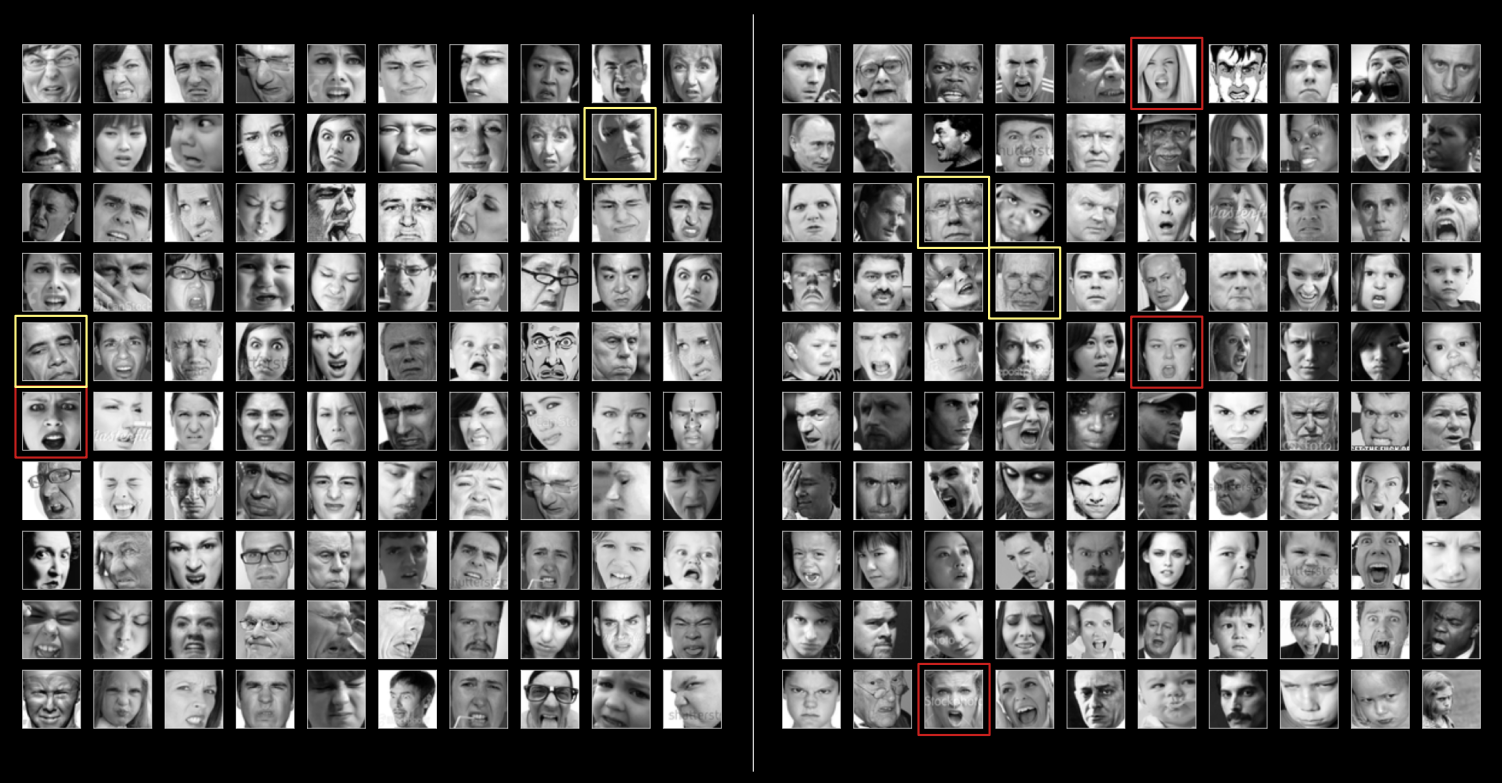
\includegraphics[width=14cm]{gambar/fer2013_disgustvsangry.png}
    \caption{Beberapa Contoh Kemiripan Data Gambar Wajah Berlabel Emosi \textit{Disgust} (Kiri) dan \textit{Angry} (Kanan) pada FER-2013}
    \label{fig:disgustvsangry}
\end{figure}
\begin{figure}[t]
    \centering
    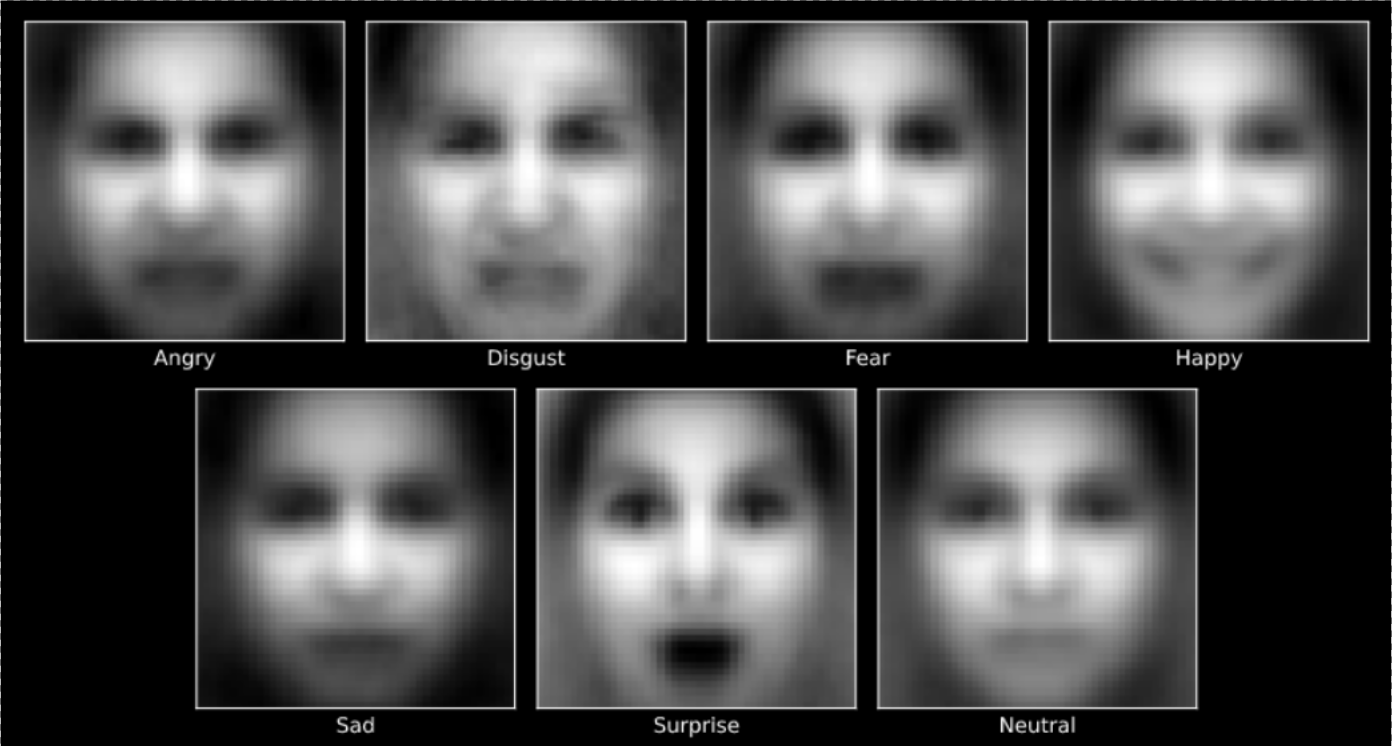
\includegraphics[width=14cm]{gambar/fer2013_rerata_gambar_per_label.png}
    \caption{Rerata Seluruh Data Gambar Wajah pada FER-2013 Per Label Emosi}
    \label{fig:reratagambarfer2013}
\end{figure}
Ada beberapa pertanyaan yang muncul setelah melihat \textit{confusion matrix} pada Gambar \ref{fig:grafikeksperimen2}. Pertama, yang mana merupakan hal yang paling mencolok, model tidak pernah berhasil dalam mengenali emosi berlabel \textit{disgust}. Apakah karena data \textit{training}-nya terlalu sedikit? Lalu jika dilihat secara saksama, emosi \textit{disgust} lebih banyak dikenali sebagai \textit{angry}. Apakah karena emosi \textit{disgust} sulit dibedakan dari \textit{angry}? Untuk itu, penulis melakukan pembandingan beberapa sampel data dari kedua label emosi tersebut yang dapat dilihat pada Gambar \ref{fig:disgustvsangry}. Di sana terlihat beberapa data gambar yang telah ditandai ternyata memang agak sulit untuk dibedakan oleh penulis secara manual sekalipun. Namun hanya dengan ini, penulis tidak bisa serta-merta menyimpulkan bahwa terdapat kesalahan dalam pelabelan set data FER-2013. Kemudian penulis mencoba melakukan pendekatan yang berbeda untuk menjawab persoalan ini, yaitu dengan menghitung rerata gambar wajah per label emosi. Berdasarkan Gambar \ref{fig:reratagambarfer2013}, penulis menyimpulkan bahwa sebenarnya meskipun terdapat beberapa gambar yang terlihat sangat mirip, namun secara keseluruhan data gambar per label masih dapat dibedakan. Kedua, data berlabel \textit{fear} belum mampu seperempatnya dikenali oleh model. Malahan lebih banyak dikenali sebagai emosi \textit{sad}. Sedangkan untuk data berlabel lain \textit{sad} dan \textit{neutral} masih belum mampu dikenali separuhnya. Penulis menduga bahwa hal ini akibat dari kurangnya kompleksitas model \textit{learning}. Oleh karena itu, penulis bersemangat untuk melanjutkan eksperimen ke skenario yang berikutnya. Secara keseluruhan, performa model rekognisi untuk tiap-tiap label emosi mengalami kenaikan. Gambar \ref{fig:perbandinganeksperimen1dan2} merangkum peningkatan tersebut berdasarkan Gambar \ref{fig:confusionmatrixeksperimen1} dan \ref{fig:confusionmatrixeksperimen2}.

\subsection{Modifikasi \acrshort{cnn} \textit{Baseline} Menjadi \acrshort{gcn}}
\begin{figure}[t]
    \centering
    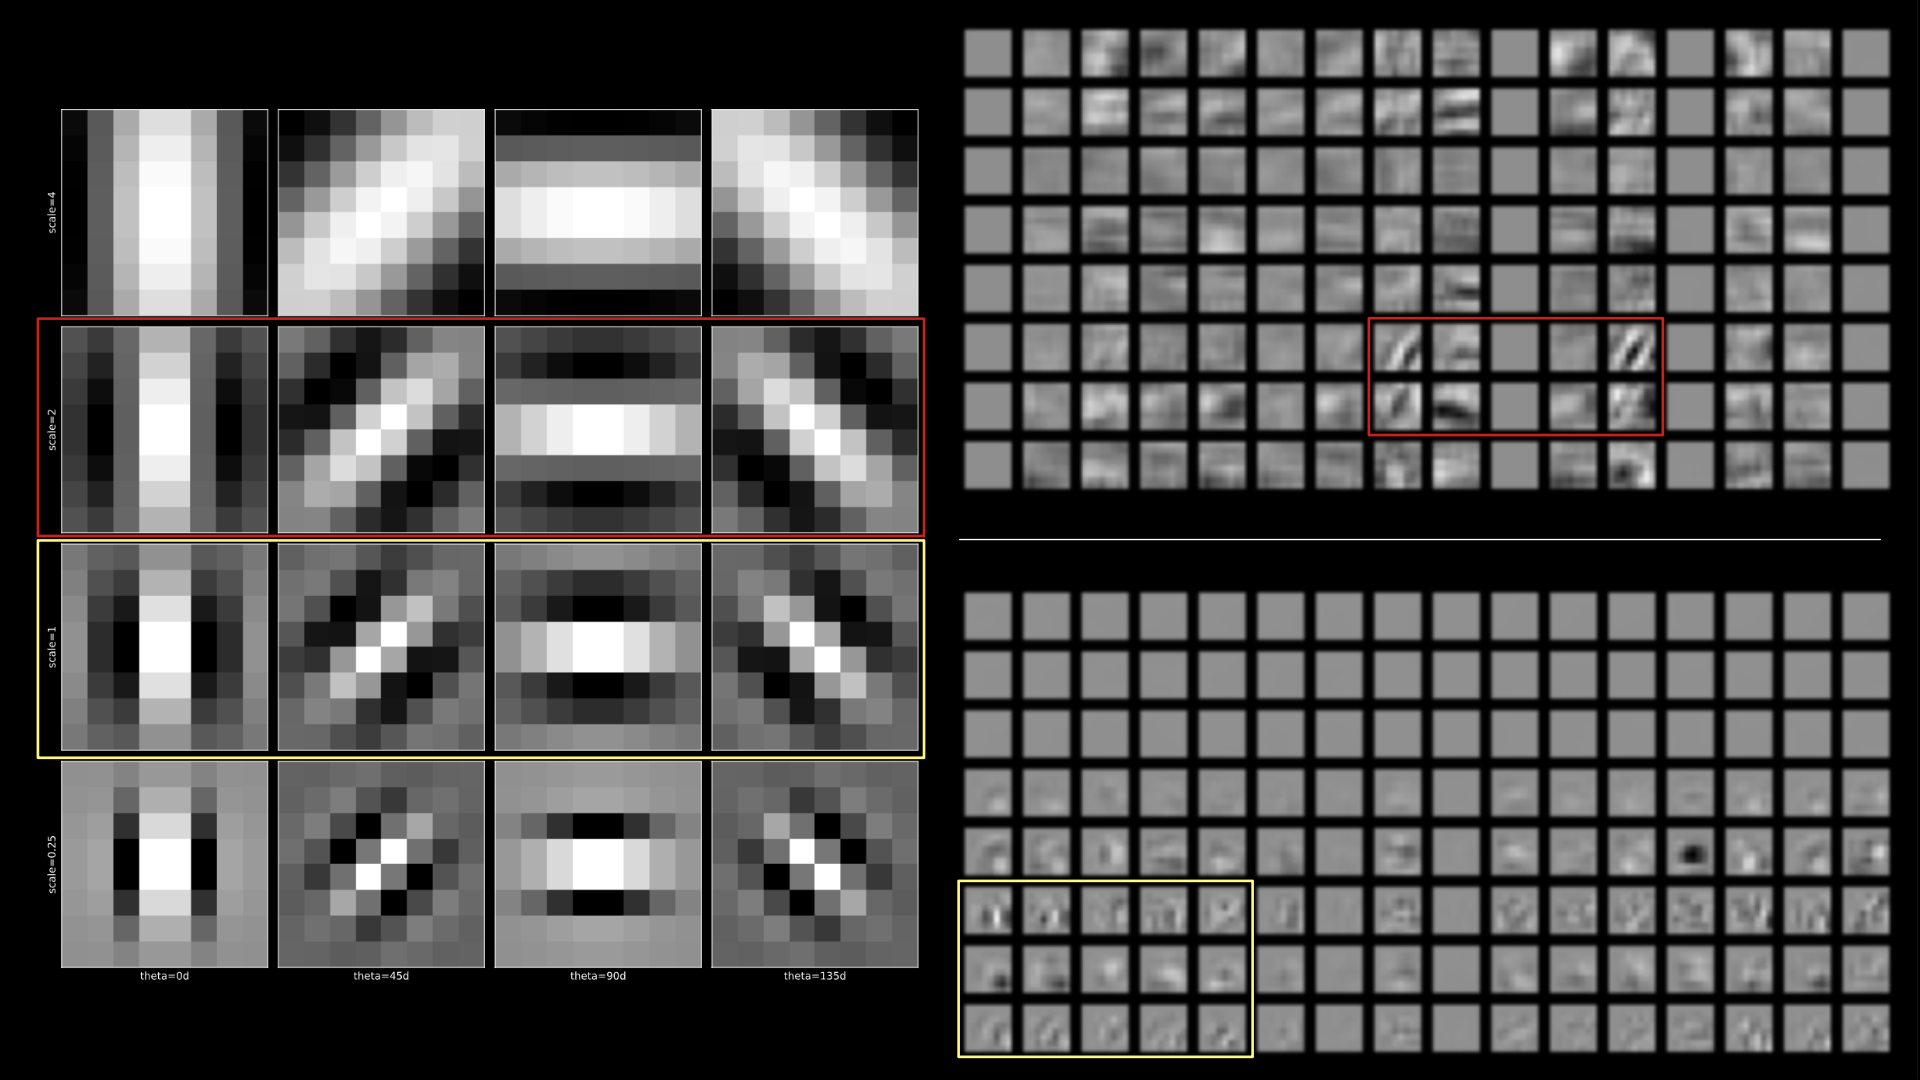
\includegraphics[width=14cm]{gambar/visualisasi_kernel_lapisan8dan9.png}
    \caption{Beberapa Contoh Kemiripan Filter Gabor (Kiri) dengan Kernel dari Lapisan Konvolusi Ke-8 (Kanan Atas) dan Ke-9 (Kanan Bawah) pada Model \acrshort{cnn} \textit{Baseline}}
    \label{fig:visualisasikernel8dan9}
\end{figure}
Pada skenario ke-2 ini, penulis melakukan modifikasi arsitektur \acrshort{cnn} \textit{baseline} menjadi \acrshort{gcn} melalui: 1) pengubahan setiap lapisan konvolusi biasa menjadi lapisan konvolusi Gabor, 2) penambahan sebuah \textit{max layer} sebelum lapisan akhir dan 3) penambahan sebuah lapisan \textit{dense} (\textit{fully connected layer}) di bagian paling akhir dalam arsitektur model.

Pada arsitektur \acrshort{gcn}, terdapat dua parameter tambahan yang perlu ditentukan, yaitu $M$ dan \textit{scale}. $M$ adalah parameter yang menentukan banyaknya variasi rotasi filter Gabor yang akan dipakai dalam rentang 0--180\degree. Jika $M = 1$, maka hanya sebuah filter Gabor pada sudut 0\degree\ yang dipakai. Jika $M > 2$, maka filter Gabor yang dipakai adalah sebanyak $M$ buah meliputi sebuah filter Gabor pada sudut 0\degree\ ditambah $M - 1$ buah filter Gabor pada rotasi yang dihitung secara kumulatif menurut $\theta = (i/M) \times 180\degree$ di mana $i$ adalah indeks urutan filter Gabor yang dimulai dari $i = 1$. Sedangkan \textit{scale} adalah skala filter Gabor relatif terhadap ukuran kernel yang dipakai pada setiap lapisan konvolusi, yaitu $8 \times 8$. Dari enam belas lapisan konvolusi pada arsitektur \textit{baseline}, penulis mengelompokkannya menjadi empat grup secara berurutan. Kemudian penulis melakukan \textit{training} pada model \acrshort{cnn} \textit{baseline} yang telah diubah menjadi \acrshort{gcn} melalui pencacahan konfigurasi parameter $M$ dalam rentang nilai 1--4 dan \textit{scale} dalam rentang nilai yang sama. Dari situ penulis dapat menyimpulkan bahwa parameter yang optimal untuk kasus ini adalah $M = 4$ dengan $\text{scale} = 2$ untuk lapisan konvolusi ke-1 hingga ke-8 dan $\text{scale} = 1$ untuk lapisan konvolusi yang lain. Hal ini dapat dijelaskan melalui visualisasi kernel pada setiap lapisan konvolusi, di mana kernel pada lapisan konvolusi ke-8 ke bawah mirip dengan filter Gabor pada $\text{scale} = 2$ dan kernel pada lapisan konvolusi ke-9 ke atas mirip dengan filter Gabor pada $\text{scale} = 1$. Pada Gambar \ref{fig:visualisasikernel8dan9} diperlihatkan beberapa contoh kemiripan tersebut. Pada bagian kiri, ditampilkan empat baris filter Gabor dengan parameter \textit{scale} yang berbeda pada empat rotasi yang berbeda. Pada bagian kanan, dari atas ke bawah, menunjukkan separuh kernel dari lapisan konvolusi ke-8 dan ke-9 secara berurutan.

\begin{table}[!t]
    \caption[Perbandingan Performa Model \acrshort{cnn} \textit{Baseline} dan \acrshort{gcn}]{Perbandingan Performa Model \acrshort{cnn} Baseline dan \acrshort{gcn}}
    \label{tab:eksperimengcn}
    \begin{tabular}{|L{5.4cm}|C{2.6cm}|C{1.5cm}|C{2.7cm}|}
        \hline
        & Akurasi (\%)$^\bigtriangleup$ & \textit{Epoch} & Waktu (jam)$^\bigtriangledown$ \\
        \hline\hline
        Model \acrshort{cnn} \textit{baseline} & 60,27 & 174 & 1,64 \\
        \hline
        Model \acrshort{gcn} & 63,51 & 150 & 7,95 \\
        \hline
    \end{tabular}
    \footnotesize
    {\raggedright Akurasi---akurasi model pada \textit{testing}; \textit{Epoch}---banyak \textit{epoch} yang dibutuhkan agar model menjadi optimal; Waktu---waktu yang dibutuhkan agar model menjadi optimal; $^\bigtriangleup$Lebih tinggi lebih baik; $^\bigtriangledown$Lebih rendah lebih baik.}
\end{table}
\begin{figure}[ht]
    \centering
    \begin{subfigure}[t]{6.75cm}
        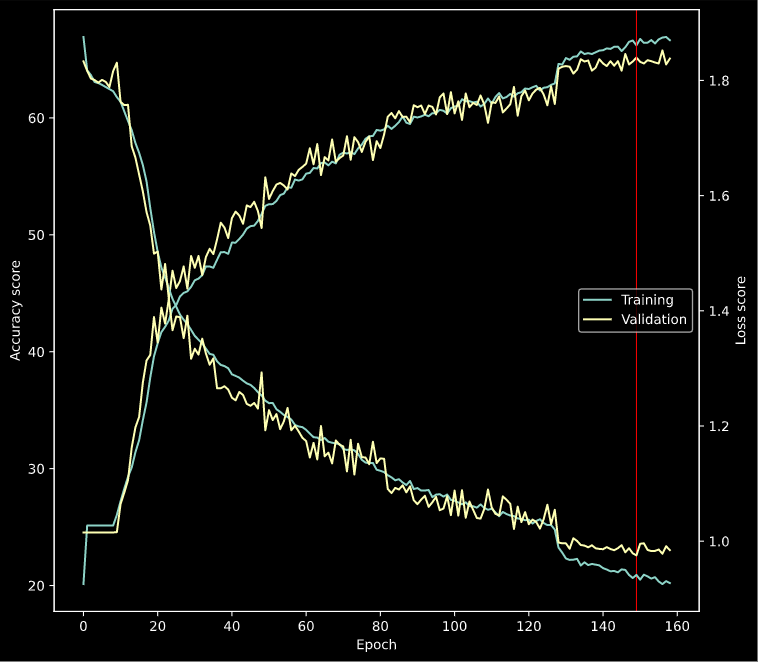
\includegraphics[width=6.75cm]{gambar/eksperimen3_grafik1.png}
        \caption{Grafik Performa Per \textit{Epoch} untuk Model \acrshort{gcn}}
        \label{fig:grafikeksperimen3}
    \end{subfigure}
    ~~~
    \begin{subfigure}[t]{6.75cm}
        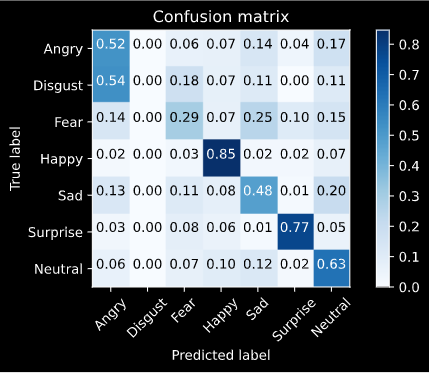
\includegraphics[width=6.75cm]{gambar/eksperimen2_matriks1.png}
        \caption{\textit{Confusion Matrix} Performa Model \acrshort{gcn}}
        \label{fig:confusionmatrixeksperimen3}
    \end{subfigure}
    \caption{Performa Model \acrshort{gcn}}
    \label{fig:hasileksperimen3}
\end{figure}
Dari eksperimen ini dibuktikan bahwa model \acrshort{gcn}, yang merupakan hasil modifikasi dari \acrshort{cnn} \textit{baseline}, memiliki performa yang lebih unggul dari pendahulunya. Sebagaimana yang terangkum dalam Tabel \ref{tab:eksperimengcn}, performa model meningkat sebesar 3,24\% disertai oleh peningkatan waktu \textit{training} sebesar 4,84 kali lipat. Di sisi lain, banyak \textit{epoch} yang harus dilalui untuk melatih model \acrshort{gcn} lebih rendah daripada sebelumnya untuk \textit{batch size} yang sama.

Sebelum membahas lebih lanjut mengenai perbandingan performa kedua model, ada dua hal yang menarik bagi penulis ketika membandingkan grafik log performa model pada Gambar \ref{fig:grafikeksperimen2} dan \ref{fig:grafikeksperimen3}. Pertama, melalui pengamatan penulis pada pengubahan parameter $M$, penggunaan arsitektur model \acrshort{gcn} selalu dimulai dengan grafik akurasi untuk \textit{training} dan \textit{validation} yang sama sekali konstan pada \textit{epoch} ke-1 hingga ke-10. Sementara itu, grafik \textit{loss} untuk \textit{training} dan \textit{validation} selalu mengalami perbaikan. Baru pada \textit{epoch} ke-10 hingga ke-25, tiap-tiap grafik mengalami perbaikan yang sangat signifikan. Sedangkan grafik log performa model yang sebelumnya relatif lebih halus setelah \textit{epoch} ke-5. Hal ini menerangkan bahwa pengenaan filter Gabor pada lapisan konvolusi \acrshort{cnn} menyulitkan mesin untuk belajar, namun memberikan wawasan yang lebih baik dalam rekognisi kelas emosi. Kedua, yang mana mengherankan penulis, grafik performa \textit{validation} hampir selalu lebih baik daripada grafik performa \textit{training} hingga \textit{epoch} tertentu di mana terlihat loncatan peningkatan yang cukup dengan jelas sesaat setelah grafik performa \textit{training} relatif mulai stabil. Jika dibandingkan dengan grafik log performa model yang paling awal pada Gambar \ref{fig:grafikeksperimen1}, hal ini menyatakan bagaimana data augmentasi dan penggunaan \textit{Gabor convolutional layer} dapat meningkatkan kemampuan generalisasi model rekognisi. Adapun kejadian di mana grafik \textit{validation} mulai konstan setelah mengalami loncatan peningkatan yang signifikan, menjelaskan bahwa hal ini terjadi akibat penulis menggunakan teknik pengecilan parameter \textit{learning rate} menggunakan fungsi \textit{reduce learning rate on plateau} dalam \textit{training} dengan faktor pengali sebesar $\sqrt{0,1}$ ketika menemukan bahwa tidak ada peningkatan senilai tertentu pada grafik \textit{validation loss} dalam sepuluh \textit{epoch} terakhir.

\begin{figure}[t]
    \centering
    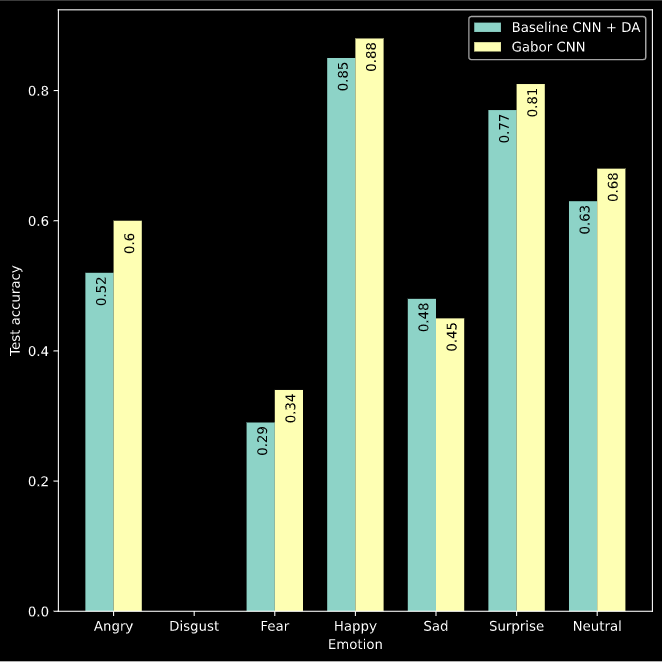
\includegraphics[width=10cm]{gambar/eksperimen2vs3_grafik1.png}
    \caption{Perbandingan Performa Model \acrshort{cnn} \textit{Baseline}\\dan \acrshort{gcn} Per Kelas Emosi}
    \label{fig:perbandinganeksperimen2dan3}
\end{figure}
Secara umum, pengadopsian arsitektur \acrshort{gcn} telah berhasil meningkatkan performa model rekognisi per kelas emosi, seperti yang diperlihatkan pada Gambar \ref{fig:perbandinganeksperimen2dan3}. Performa model meningkat untuk setiap label emosi kecuali \textit{disgust} dan \textit{fear}. Berulang lagi tidak ada perbaikan apapun dalam pengenalan emosi \textit{disgust}. Bahkan jika membandingkan \textit{confusion matrix} pada Gambar \ref{fig:confusionmatrixeksperimen2} dan \ref{fig:confusionmatrixeksperimen3}, data berlabel \textit{disgust} malah lebih banyak lagi dikenali sebagai \textit{angry}. Sehingga penulis berakhir pada kesimpulan bahwa ketimpangan yang sangat jelas terjadi pada banyak data berlabel emosi \textit{disgust} telah menyebabkan kegagalan model dalam mengenali emosi tersebut. Sementara kemampuan model dalam mengenali emosi \textit{sad} menjadi sedikit berkurang.

\subsection{Modifikasi \acrshort{gcn} Menjadi \textit{Ensemble} \acrshort{gcns}}
Pada skenario ini, penulis mencoba membangun \textit{ensemble network} menggunakan dua teknik yang berbeda. Teknik yang pertama merupakan teknik \textit{ensemble} konvensional, yaitu penggabungan hasil prediksi secara terpisah dari setiap model yang dilatih menggunakan bagian wajah tertentu. Hasil prediksi akhir untuk sebuah input gambar baru dihitung menggunakan rumus statistik tertentu, yaitu \textit{simple average} dan \textit{weighted average}. \textit{Simple average} diperoleh melalui operasi perhitungan rata-rata biasa pada (\ref{equ:average}),
\begin{equation}
    \bar{y} = \frac{y_{\text{i}} + y_{\text{j}}}{2}
    \label{equ:average}
\end{equation}
sedangkan \textit{weighted average} diperoleh dari (\ref{equ:waverage}),
\begin{equation}
    \bar{y} = \frac{y_{\text{i}} * a_{\text{i}} + y_{\text{j}} * a_{\text{j}}}{a_{\text{i}} + a_{\text{i}}}
    \label{equ:waverage}
\end{equation}
di mana $y$ adalah larik probabilitas berdimensi $1 \times 7$ hasil prediksi sebuah input baru dan $a$ adalah akurasi tes untuk masing-masing model $i$ dan $j$ yang berbeda. Sejujurnya, alangkah lebih baik jika \textit{weighted average} dihitung dengan mempertimbangkan akurasi tes per kelas pada \textit{confusion matrix}. Namun penulis kesulitan menghitungnya, sebab model sama sekali tidak bisa memprediksi data berlabel \textit{disgust}. Sementara teknik yang kedua bekerja dengan menggabungkan arsitektur jaringan sebanyak $n$ menjadi jaringan bertingkat (\textit{cascaded network}), di mana $n$ adalah banyak bagian wajah yang disegmentasi.

Sebelum membahas hasil eksperimen pada skenario ini, perlu diketahui bahwa kali ini penulis meninggalkan fungsi \textit{reduce learning rate on plateau}. Karena menurut hasil pengamatan penulis, proses \textit{training} pada skenario ini relatif lambat dan kurang stabil. Sehingga jika penulis tetap menggunakan fungsi tersebut, proses \textit{training} hingga mencapai optimal akan sangat lambat akibat beberapa kali pengecilan \textit{learning rate} dalam rentang waktu yang sebentar.

\begin{table}[t]
    \caption{Perbandingan Performa Berbagai Kombinasi Model \textit{Ensemble} \acrshort{gcns}}
    \label{tab:eksperimengcnfrs}
    \begin{tabular}{|C{2.3cm}|C{1cm}|C{1cm}|C{1.2cm}|C{1.8cm}|C{1.8cm}|C{1.8cm}|}
        \hline
        \multicolumn{1}{|c|}{\multirow{3}{*}{Fitur}} & \multicolumn{2}{c|}{\multirow{3}{*}{Waktu (jam)$^\bigtriangledown$}} & \multicolumn{1}{c|}{\multirow{3}{*}{\textit{Epoch}}} & \multicolumn{3}{c|}{Akurasi \textit{Testing} (\%)$^\bigtriangleup$} \\
        \cline{5-7}
        & \multicolumn{2}{c|}{} &  & \multirow{2}{*}{\textit{Single}} & \textit{Simple Average} & \textit{Weighted Average} \\
        \hline\hline
        \multirow{2}{*}{EN + NM} & 4,17 & \multirow{2}{*}{8,87} & 124 & 58,09 & \multirow{2}{*}{62,20} & \multirow{2}{*}{62,20} \\
        \cline{2-2}\cline{4-5}
        & 4,70 &  & 141 & 58,06 &  &  \\
        \hline
        \multirow{3}{*}{E + N + M} & 3,44 & \multirow{3}{*}{10,34} & 153 & 17,41 & \multirow{3}{*}{44,10} & \multirow{3}{*}{53,22} \\
        \cline{2-2}\cline{4-5}
        & 4,05 &  & 181 & 25,45 &  &  \\
        \cline{2-2}\cline{4-5}
        & 2,85 &  & 129 & 53,88 &  &  \\
        \hline
        E + N & \multirow{3}{*}{Ibid.} & 7,49 & \multicolumn{2}{c|}{\multirow{3}{*}{Ibid.}} & 17,74 & 17,62 \\
        \cline{1-1}\cline{3-3}\cline{6-7}
        N + M &  & 6,90 & \multicolumn{2}{c|}{} & 52,77 & 53,61 \\
        \cline{1-1}\cline{3-3}\cline{6-7}
        E + M &  & 6,29 & \multicolumn{2}{c|}{} & 44,91 & 53,28 \\
        \hline\hline
        EN + NM (\textit{concat.}) & \multicolumn{2}{c|}{\multirow{2}{*}{7,34}} & \multirow{2}{*}{103} & \multirow{2}{*}{59,71} & \multicolumn{2}{c|}{\multirow{4}{*}{-}} \\
        \cline{1-5}
        E + N + M (\textit{concat.}) & \multicolumn{2}{c|}{\multirow{2}{*}{8,36}} & \multirow{2}{*}{131} & \multirow{2}{*}{54,12} & \multicolumn{2}{c|}{} \\
        \hline\hline
        ENM & \multicolumn{2}{c|}{6,80} & 131 & 62,08 & \multicolumn{2}{c|}{-} \\
        \hline
    \end{tabular}
    \footnotesize
    {\raggedright E---(\textit{Eyes}) area bagian kedua mata; N---(\textit{Nose}) area bagian hidung; M---(\textit{Mouth}) area bagian mulut;\\
    \textit{Epoch}---banyak \textit{epoch} yang dibutuhkan agar model menjadi optimal; Waktu---waktu yang dibutuhkan agar model menjadi optimal; $^\bigtriangleup$Lebih tinggi lebih baik; $^\bigtriangledown$Lebih rendah lebih baik.}
\end{table}
\begin{figure}[t]
    \centering
    \begin{subfigure}[t]{6.75cm}
        \includegraphics[width=6.75cm]{gambar/eksperimen4b1_grafik1.png}
        \caption{Grafik Performa Per \textit{Epoch} untuk Model EN}
        \label{fig:grafikeksperimen4b11}
    \end{subfigure}
    ~~~
    \begin{subfigure}[t]{6.75cm}
        \includegraphics[width=6.75cm]{gambar/eksperimen4b1_matriks1.png}
        \caption{\textit{Confusion Matrix} Performa Model EN}
        \label{fig:confusionmatrixeksperimen4b11}
    \end{subfigure}
    ~~~
    \begin{subfigure}[t]{6.75cm}
        \includegraphics[width=6.75cm]{gambar/eksperimen4b1_grafik2.png}
        \caption{Grafik Performa Per \textit{Epoch} untuk Model NM}
        \label{fig:grafikeksperimen4b12}
    \end{subfigure}
    ~~~
    \begin{subfigure}[t]{6.75cm}
        \includegraphics[width=6.75cm]{gambar/eksperimen4b1_matriks2.png}
        \caption{\textit{Confusion Matrix} Performa Model NM}
        \label{fig:confusionmatrixeksperimen4b12}
    \end{subfigure}
    \caption{Performa Model \acrshort{gcns} Menggunakan Fitur EN + NM}
    \label{fig:hasileksperimen4b1}
\end{figure}
\begin{figure}[t]
    \ContinuedFloat
    \centering
    \begin{subfigure}[t]{6.75cm}
        \includegraphics[width=6.75cm]{gambar/eksperimen4b1_matriks3.png}
        \caption{\textit{Confusion Matrix} Performa Model EN + NM Berdasarkan Perhitungan \textit{Simple Average}}
        \label{fig:confusionmatrixeksperimen4b13}
    \end{subfigure}
    ~~~
    \begin{subfigure}[t]{6.75cm}
        \includegraphics[width=6.75cm]{gambar/eksperimen4b1_matriks4.png}
        \caption{\textit{Confusion Matrix} Performa Model EN + NM Berdasarkan Perhitungan \textit{Weighted Average}}
        \label{fig:confusionmatrixeksperimen4b14}
    \end{subfigure}
    \caption{Performa Model \acrshort{gcns} Menggunakan Fitur EN + NM (Lanjutan)}
\end{figure}
Secara khusus, salah satu tujuan dari skenario ini adalah menjawab sebuah \textit{future work} penelitian terkait demi mengembangkan model rekognisi yang andal menggunakan teknik \acrshort{frs} untuk mampu mengenali emosi dari gambar wajah manusia yang diputar pada sudut berapa pun \shortcite{islam2018facial2}. Hasil dari tiap-tiap eksperimen pada skenario ini terangkum pada Tabel \ref{tab:eksperimengcnfrs}. Pada kolom akurasi \textit{testing}, terlihat bahwa pemodelan menggunakan set data hasil \acrshort{frs} dua bagian wajah (EN + NM) memiliki akurasi yang paling tinggi; jauh lebih baik daripada pemodelan menggunakan tiga bagian wajah (E + N + M) dan kombinasi dua-dua (E + N, N + M dan E + M), baik menggunakan teknik \textit{ensemble} yang pertama maupun yang kedua. Kendati pun akurasinya masih lebih rendah ketimbang model yang dilatih tanpa memanfaatkan teknik \acrshort{frs} (model terbaik pada skenario sebelumnya), namun penurunannya hanya sebesar 1,31\%. Sementara pemodelan menggunakan tiga area wajah dan kombinasi dua-dua tidak bisa diandalkan, bahkan performanya jauh lebih rendah daripada model \textit{baseline}.

Lebih jauhnya, jika ditilik setiap \emph{confusion matrix} yang ditunjukkan pada Gambar \ref{fig:confusionmatrixeksperimen4b11}--\ref{fig:confusionmatrixeksperimen4b8}, maka dapat disimpulkan beberapa poin. Dalam membandingkan masing-masing dari performa model EN dan NM, tampak bahwa model EN memiliki akurasi yang lebih tinggi pada pengenalan emosi \textit{angry} dan \textit{surprise}. Untuk pengenalan emosi \textit{angry}, model EN jauh lebih baik dari model NM dengan selisih 22\%. Sehingga jelas bahwa emosi \textit{angry} lebih mudah dikenali menggunakan bagian wajah atas manusia. Sedangkan model NM relatif sedikit lebih baik pada sisanya. Khusus untuk \textit{disgust}, model EN lebih banyak melakukan kesalahan prediksi sebagai \textit{angry} dengan selisih 30\%. Hal ini menjelaskan bahwa emosi \textit{disgust} lebih sulit dikenali menggunakan bagian wajah atas manusia. Untuk emosi \textit{fear}, dapat disimpulkan bahwa emosi ini lebih sulit dikenali dengan melihat bagian atas dan bawah wajah secara terpisah.

Di sisi lain, performa model EN + NM dalam perhitungan dua teknik rerata memberikan \textit{confusion matrix} yang tepat sama seperti yang terlihat pada Gambar \ref{fig:confusionmatrixeksperimen4b13} dan \ref{fig:confusionmatrixeksperimen4b14}. Untuk setiap label emosi, kombinasi kedua model ini mampu memberikan nilai akurasi yang sedikit lebih baik dibandingkan model NM. Namun untuk label \textit{angry}, akurasinya 5\% lebih rendah daripada model EN. Sementara penyimpangan prediksi emosi \textit{disgust} mendekati kemampuan model EN.

\begin{figure}[t]
    \centering
    \begin{subfigure}[t]{6.75cm}
        \includegraphics[width=6.75cm]{gambar/eksperimen4b2_grafik1.png}
        \caption{Grafik Performa Per \textit{Epoch} untuk Model E}
        \label{fig:grafikeksperimen4b21}
    \end{subfigure}
    ~~~
    \begin{subfigure}[t]{6.75cm}
        \includegraphics[width=6.75cm]{gambar/eksperimen4b2_matriks1.png}
        \caption{\textit{Confusion Matrix} Performa Model E}
        \label{fig:confusionmatrixeksperimen4b21}
    \end{subfigure}
    ~~~
    \begin{subfigure}[t]{6.75cm}
        \includegraphics[width=6.75cm]{gambar/eksperimen4b2_grafik2.png}
        \caption{Grafik Performa Per \textit{Epoch} untuk Model N}
        \label{fig:grafikeksperimen4b22}
    \end{subfigure}
    ~~~
    \begin{subfigure}[t]{6.75cm}
        \includegraphics[width=6.75cm]{gambar/eksperimen4b2_matriks2.png}
        \caption{\textit{Confusion Matrix} Performa Model N}
        \label{fig:confusionmatrixeksperimen4b22}
    \end{subfigure}
    \caption{Performa Model \acrshort{gcns} Menggunakan Fitur E + N + M}
    \label{fig:hasileksperimen4b2}
\end{figure}
\begin{figure}[!htb]
    \ContinuedFloat
    \centering
    \begin{subfigure}[t]{6.75cm}
        \includegraphics[width=6.75cm]{gambar/eksperimen4b2_grafik3.png}
        \caption{Grafik Performa Per \textit{Epoch} untuk Model M}
        \label{fig:grafikeksperimen4b23}
    \end{subfigure}
    ~~~
    \begin{subfigure}[t]{6.75cm}
        \includegraphics[width=6.75cm]{gambar/eksperimen4b2_matriks3.png}
        \caption{\textit{Confusion Matrix} Performa Model M}
        \label{fig:confusionmatrixeksperimen4b23}
    \end{subfigure}
    ~~~
    \begin{subfigure}[t]{6.75cm}
        \includegraphics[width=6.75cm]{gambar/eksperimen4b2_matriks4.png}
        \caption{\textit{Confusion Matrix} Performa Model E + N + M Berdasarkan Perhitungan \textit{Simple Average}}
        \label{fig:confusionmatrixeksperimen4b24}
    \end{subfigure}
    ~~~
    \begin{subfigure}[t]{6.75cm}
        \includegraphics[width=6.75cm]{gambar/eksperimen4b2_matriks5.png}
        \caption{\textit{Confusion Matrix} Performa Model E + N + M Berdasarkan Perhitungan \textit{Weighted Average}}
        \label{fig:confusionmatrixeksperimen4b25}
    \end{subfigure}
    \caption{Performa Model \acrshort{gcns} Menggunakan Fitur E + N + M (Lanjutan)}
\end{figure}
Dalam membandingkan masing-masing dari performa model E, N dan M, terlihat pada Gambar \ref{fig:confusionmatrixeksperimen4b21}--\ref{fig:confusionmatrixeksperimen4b23} bahwa untuk model E dan N memiliki \textit{confusion matrix} yang tidak menarik dan masuk akal. Model E hanya mampu mengenali emosi \textit{angry}, \textit{happy} dan \textit{sad} pada akurasi yang kurang dari 30\%. Sedangkan untuk emosi sisanya tersebar dengan cukup merata pada ketiga label emosi tersebut. Emosi \textit{surprise} dan \textit{neutral} yang umumnya termasuk kelas yang paling mudah untuk dikenali, tidak mampu diprediksi oleh model E. Selanjutnya yang sangat mengejutkan adalah model N hanya mampu mengenali emosi \textit{happy} secara 100\% akurat. Namun, label emosi lainnya juga 100\% gagal diprediksi dan malah dianggap sebagai \textit{happy}. Kemudian untuk model M, performanya dalam mengenali setiap emosi cukup dapat diterima. Sebab memberikan \textit{confusion matrix} yang mirip dengan model \textit{baseline} tanpa augmentasi data.

Di sisi lain, rerata performa model E + N + M memberikan \textit{confusion matrix} yang cukup mirip dengan performa model M. Terutama dalam perhitungan \textit{weighted average}, model memberikan akurasi yang sedikit lebih baik pada pengenalan emosi \textit{angry} dan \textit{fear}. Sedangkan untuk sisanya relatif menurun sedikit.

Dari analisis di atas, diketahui bahwa ketiga fitur wajah tersebut ternyata saling berkaitan satu sama lain pada pengenalan emosi manusia. Namun area bagian mulut memang memberikan kontribusi paling besar dari keseluruhan skenario yang dilakukan. Di sisi lain, rendahnya akurasi model rekognisi emosi untuk tiap-tiap bagian wajah terpisah mengungkapkan bahwa di antara kemungkinan sebabnya adalah adanya perbedaan yang kuat antara orang barat dan timur dalam bagaimana mereka mengekspresikan suatu emosi \shortcite{benitez2017analysis}.

\begin{figure}[t]
    \centering
    \begin{subfigure}[t]{6.75cm}
        \includegraphics[width=6.75cm]{gambar/eksperimen4b3_matriks1.png}
        \caption{\textit{Confusion Matrix} Performa Model E + N Berdasarkan Perhitungan \textit{Simple Average}}
        \label{fig:confusionmatrixeksperimen4b3}
    \end{subfigure}
    ~~~
    \begin{subfigure}[t]{6.75cm}
        \includegraphics[width=6.75cm]{gambar/eksperimen4b3_matriks2.png}
        \caption{\textit{Confusion Matrix} Performa Model E + N Berdasarkan Perhitungan \textit{Weighted Average}}
        \label{fig:confusionmatrixeksperimen4b3}
    \end{subfigure}
    \caption{Performa Model \acrshort{gcns} Menggunakan Fitur E + N}
    \label{fig:hasileksperimen4b3}
\end{figure}

\begin{figure}[t]
    \centering
    \begin{subfigure}[t]{6.75cm}
        \includegraphics[width=6.75cm]{gambar/eksperimen4b4_matriks1.png}
        \caption{\textit{Confusion Matrix} Performa Model N + M Berdasarkan Perhitungan \textit{Simple Average}}
        \label{fig:confusionmatrixeksperimen4b4}
    \end{subfigure}
    ~~~
    \begin{subfigure}[t]{6.75cm}
        \includegraphics[width=6.75cm]{gambar/eksperimen4b4_matriks2.png}
        \caption{\textit{Confusion Matrix} Performa Model N + M Berdasarkan Perhitungan \textit{Weighted Average}}
        \label{fig:confusionmatrixeksperimen4b4}
    \end{subfigure}
    \caption{Performa Model \acrshort{gcns} Menggunakan Fitur N + M}
    \label{fig:hasileksperimen4b4}
\end{figure}

\begin{figure}[t]
    \centering
    \begin{subfigure}[t]{6.75cm}
        \includegraphics[width=6.75cm]{gambar/eksperimen4b5_matriks1.png}
        \caption{\textit{Confusion Matrix} Performa Model E + M Berdasarkan Perhitungan \textit{Simple Average}}
        \label{fig:confusionmatrixeksperimen4b5}
    \end{subfigure}
    ~~~
    \begin{subfigure}[t]{6.75cm}
        \includegraphics[width=6.75cm]{gambar/eksperimen4b5_matriks2.png}
        \caption{\textit{Confusion Matrix} Performa Model E + M Berdasarkan Perhitungan \textit{Weighted Average}}
        \label{fig:confusionmatrixeksperimen4b5}
    \end{subfigure}
    \caption{Performa Model \acrshort{gcns} Menggunakan Fitur E + M}
    \label{fig:hasileksperimen4b5}
\end{figure}

\begin{figure}[t]
    \centering
    \begin{subfigure}[t]{6.75cm}
        \includegraphics[width=6.75cm]{gambar/eksperimen4b6_grafik1.png}
        \caption{Grafik Performa Per \textit{Epoch} untuk Model EN + NM (\textit{Concat.})}
        \label{fig:confusionmatrixeksperimen4b6}
    \end{subfigure}
    ~~~
    \begin{subfigure}[t]{6.75cm}
        \includegraphics[width=6.75cm]{gambar/eksperimen4b6_matriks1.png}
        \caption{\textit{Confusion Matrix} Performa Model EN + NM (\textit{Concat.})}
        \label{fig:confusionmatrixeksperimen4b6}
    \end{subfigure}
    \caption{Performa Model \acrshort{gcns} Menggunakan Fitur EN + NM (\textit{Concat.})}
    \label{fig:hasileksperimen4b6}
\end{figure}

\begin{figure}[t]
    \centering
    \begin{subfigure}[t]{6.75cm}
        \includegraphics[width=6.75cm]{gambar/eksperimen4b7_grafik1.png}
        \caption{Grafik Performa Per \textit{Epoch} untuk Model E + N + M (\textit{Concat.})}
        \label{fig:confusionmatrixeksperimen4b7}
    \end{subfigure}
    ~~~
    \begin{subfigure}[t]{6.75cm}
        \includegraphics[width=6.75cm]{gambar/eksperimen4b7_matriks1.png}
        \caption{\textit{Confusion Matrix} Performa Model E + N + M (\textit{Concat.})}
        \label{fig:confusionmatrixeksperimen4b7}
    \end{subfigure}
    \caption{Performa Model \acrshort{gcns} Menggunakan Fitur E + N + M (\textit{Concat.})}
    \label{fig:hasileksperimen4b7}
\end{figure}

\begin{figure}[!t]
    \centering
    \begin{subfigure}[t]{6.75cm}
        \includegraphics[width=6.75cm]{gambar/eksperimen4b8_grafik1.png}
        \caption{Grafik Performa Per \textit{Epoch} untuk Model ENM}
        \label{fig:confusionmatrixeksperimen4b8}
    \end{subfigure}
    ~~~
    \begin{subfigure}[t]{6.75cm}
        \includegraphics[width=6.75cm]{gambar/eksperimen4b8_matriks1.png}
        \caption{\textit{Confusion Matrix} Performa Model ENM}
        \label{fig:confusionmatrixeksperimen4b8}
    \end{subfigure}
    \caption{Performa Model \acrshort{gcns} Menggunakan Fitur ENM}
    \label{fig:hasileksperimen4b8}
\end{figure}

Meskipun penggunaan fitur bagian mulut memberikan akurasi yang relatif lebih baik daripada yang lain, namun penggabungan dengan fitur lain (area bagian mata dan hidung) malah mengurangi sedikit performa model rekognisi. Di mana model N + M memberikan penurunan yang cukup signifikan pada pengenalan emosi \textit{sad} dengan selisih akurasi 13\%. Akan tetapi untuk emosi \textit{angry}, \textit{fear}, \textit{happy} dan \textit{neutral} meningkat sedikit berturut-turut sebesar 1\%, 3\%, 1\% dan 6\%. Sementara itu, model E + M hanya memberikan peningkatan yang sedikit pada emosi \textit{fear}, \textit{happy} dan \textit{sad} berturut-turut sebesar 5\%, 1\% dan 2\%. Namun mengalami penurunan sebesar 7\% untuk emosi \textit{surprise} dan \textit{neutral}.

Hal ini mungkin terjadi sebagai akibat dari sangat jeleknya akurasi model pada set data bagian mata dan hidung secara terpisah, terutama untuk bagian mata. Sehingga meskipun akurasi model dihitung secara proporsional, performa model menjadi sedikit menurun. Fenomena penurunan performa ini diperkuat oleh perbandingan hasil perhitungan akurasi menggunakan dua teknik yang berbeda, di mana perhitungan \textit{simple average} yang tidak proporsional hampir selalu memberikan nilai akurasi yang lebih rendah dari \textit{weighted average}. Sementara penggabungan fitur bagian mata dan hidung menghasilkan performa yang tidak bisa diterima.

Selanjutnya, model EN + NM yang dilatih menggunakan \textit{network ensemble} pun tidak memiliki keunggulan yang menarik dibandingkan model-model yang sebelumnya. Malahan model E + N + M yang dilatih pada \textit{network ensemble} sangat mengecewakan dalam mengenali emosi \textit{angry}. Namun satu hal yang membedakannya dari semua model sebelumnya adalah kebanyakan data tes berlabel emosi \textit{disgust} dikenali sebagai \textit{fear}. Hal ini membuka sedikit peluang peningkatan performa model dalam mengenali \textit{disgust}, yaitu bahwa sebetulnya tidak benar jika \textit{disgust} ini tidak dapat dibedakan dari \textit{angry}.

Sebagai pertimbangan lain, pada skenario ini dilakukan \textit{training} pada set data hasil \textit{cropping} area wajah penuh, yaitu set data yang disimpan sesaat sebelum masuk ke dalam proses \acrshort{frs}. Sayangnya, teknik \textit{cropping} ini ternyata tidak membuat performa model lebih baik ketimbang tanpa \textit{cropping}. Di sisi lain, tanpa harus mengorbankan performa yang cukup berarti, teknik ini lebih disukai daripada pemodelan menggunakan teknik \acrshort{frs}, sebab membutuhkan waktu \textit{training} yang relatif lebih cepat.

\subsection{Modifikasi Log-\acrshort{gcn} Menjadi \textit{Ensemble} Log-\acrshort{gcns}}
Pada eksperimen ini, penulis mencoba melakukan modifikasi \acrshort{gcn} melalui pengubahan filter Gabor yang dimanfaatkan dalam proses ekstraksi fitur menjadi filter log-Gabor. Namun sebelum mengeksekusi skenario eksperimen terakhir ini, penulis ingin melihat apakah pengubahan filter tersebut dapat memberikan dampak terhadap kinerja model \acrshort{gcn}, sehingga diputuskan bahwa penulis kembali menggunakan set data primer.

Konfigurasi parameter filter log-Gabor yang dipakai pada eksperimen ini dibuat menyerupai konfigurasi filter Gabor terbaik yang sebelumnya. Bedanya, untuk filter log-Gabor, penulis menentukan frekuensi spasial $\text{sf\_0} = 0,0075 / \text{scale}$ sebagai ganti atas variabel \textit{scale} pada filter Gabor. Di mana untuk lapisan konvolusi ke-8 ke bawah menggunakan $\text{scale} = 1,25$, sedangkan sisanya menggunakan $\text{scale} = 1,0$. Perbedaan yang mendasar dari kedua filter ini ditunjukkan pada Gambar \ref{fig:filterloggaborvsgabor}. Di mana bagian daerah dengan frekuensi spasial yang rendah (daerah berwarna hitam) pada filter log-Gabor cenderung cembung mengarah ke dalam. Sedangkan pada filter Gabor, daerah ini cenderung cembung mengarah ke luar.
\begin{figure}[!t]
    \centering
    \begin{subfigure}[t]{14cm}
        \includegraphics[width=14cm]{gambar/filter_loggaborvsgabor1.png}
        \caption{Filter log-Gabor Versus Gabor pada $8 \times 8$ Piksel}
        \label{fig:filterloggaborvsgabor1}
    \end{subfigure}
    ~~~
    \begin{subfigure}[t]{14cm}
        \includegraphics[width=14cm]{gambar/filter_loggaborvsgabor2.png}
        \caption{Filter log-Gabor Versus Gabor pada $100 \times 100$ Piksel}
        \label{fig:filterloggaborvsgabor2}
    \end{subfigure}
    \caption{Beberapa Contoh Perbedaan Filter log-Gabor (Kanan) dan Gabor (Kiri)}
    \label{fig:filterloggaborvsgabor}
\end{figure}

\begin{table}[t]
    \caption{Perbandingan Performa Model \acrshort{gcn} dan Log-\acrshort{gcn}}
    \label{tab:eksperimenloggcn}
    \begin{tabular}{|L{5.4cm}|C{2.6cm}|C{1.5cm}|C{2.7cm}|}
        \hline
        & Akurasi (\%)$^\bigtriangleup$ & \textit{Epoch} & Waktu (jam)$^\bigtriangledown$ \\
        \hline\hline
        Model \acrshort{gcn} & 63,51 & 150 & 7,95 \\
        \hline
        Model Log-\acrshort{gcn} & 65,13 & 155 & 8,38 \\
        \hline
    \end{tabular}
    \footnotesize
    {\raggedright Akurasi---akurasi model pada \textit{testing}; \textit{Epoch}---banyak \textit{epoch} yang dibutuhkan agar model menjadi optimal; Waktu---waktu yang dibutuhkan agar model menjadi optimal; $^\bigtriangleup$Lebih tinggi lebih baik; $^\bigtriangledown$Lebih rendah lebih baik.}
\end{table}
Hasil dari eksperimen pada skenario ini ditampilkan pada Tabel \ref{tab:eksperimenloggcn} di mana terbukti bahwa model log-\acrshort{gcn} memiliki performa yang lebih baik daripada \acrshort{gcn} dengan perbaikan yang cukup jelas pada data berlabel \textit{sad} (Gambar \ref{fig:perbandinganeksperimen3dan5a}). Untuk mendapatkan peningkatan sebesar 1,62\% pada akurasi \textit{testing}, model log-\acrshort{gcn} memerlukan waktu \textit{training} 1,05 kali lebih lama. Model ini menjadi model dengan performa terbaik di atas semua skenario pemodelan pada penelitian ini. Peningkatan akurasi ini bukan akibat dari kebetulan melakukan \emph{training} pada kondisi mesin sedemikian rupa. Sebab berdasarkan dari percobaan tiga kali \emph{training} untuk masing-masing skenario utama pada penelitian ini, biasanya perbedaan akurasi antara model paling buruk dan paling baik berkisar di bawah angka 1,0\%. Kemudian yang amat disayangkan di sini adalah model yang dilatih hingga saat ini masih belum mampu untuk mengenali data berlabel \textit{disgust} dengan benar sama sekali sebagaimana yang ditunjukkan oleh \textit{confusion matrix} pada Gambar \ref{fig:confusionmatrixeksperimen5a}.
\begin{figure}[t]
    \centering
    \begin{subfigure}[t]{6.75cm}
        \includegraphics[width=6.75cm]{gambar/eksperimen5a_grafik1.png}
        \caption{Grafik Performa Per \textit{Epoch} untuk Model Log-\acrshort{gcn}}
        \label{fig:confusionmatrixeksperimen5a}
    \end{subfigure}
    ~~~
    \begin{subfigure}[t]{6.75cm}
        \includegraphics[width=6.75cm]{gambar/eksperimen5a_matriks1.png}
        \caption{\textit{Confusion Matrix} Performa Model Log-\acrshort{gcn}}
        \label{fig:confusionmatrixeksperimen5a}
    \end{subfigure}
    \caption{Performa Model Log-\acrshort{gcn}}
    \label{fig:hasileksperimen5a}
\end{figure}
\begin{figure}[t]
    \centering
    \includegraphics[width=10cm]{gambar/eksperimen3vs5_grafik1.png}
    \caption{Perbandingan Performa Model \acrshort{gcn} dan\\Log-\acrshort{gcn} Per Kelas Emosi}
    \label{fig:perbandinganeksperimen3dan5a}
\end{figure}

Setelah mengetahui bahwa pengubahan filter Gabor menjadi log-Gabor berhasil meningkatkan performa model, penulis melakukan modifikasi log-\acrshort{gcn} menjadi \textit{ensemble} log-\acrshort{gcns}, yaitu pengenaan teknik \acrshort{frs} terhadap arsitektur log-\acrshort{gcn}. Dari berbagai skenario implementasi teknik \acrshort{frs} pada Tabel \ref{tab:eksperimengcnfrs}, penulis mengangkat tiga pendekatan yang menghasilkan kinerja model terbaik untuk dilakukan kembali pada eksperimen tahap ini. Hasilnya diperlihatkan pada Tabel \ref{tab:eksperimenlgcnfrs}.
\begin{table}[t]
    \caption{Perbandingan Performa Berbagai Kombinasi Model \textit{Ensemble} Log-\acrshort{gcns}}
    \label{tab:eksperimenlgcnfrs}
    \begin{tabular}{|C{2.3cm}|C{1cm}|C{1cm}|C{1.2cm}|C{1.8cm}|C{1.8cm}|C{1.8cm}|}
        \hline
        \multicolumn{1}{|c|}{\multirow{3}{*}{Fitur}} & \multicolumn{2}{c|}{\multirow{3}{*}{Waktu (jam)$^\bigtriangledown$}} & \multicolumn{1}{c|}{\multirow{3}{*}{\textit{Epoch}}} & \multicolumn{3}{c|}{Akurasi \textit{Testing} (\%)$^\bigtriangleup$} \\
        \cline{5-7}
        & \multicolumn{2}{c|}{} &  & \multirow{2}{*}{\textit{Single}} & \textit{Simple Average} & \textit{Weighted Average} \\
        \hline\hline
        \multirow{2}{*}{EN + NM} & 3,71 & \multirow{2}{*}{6,91} & 114 & 59,23 & \multirow{2}{*}{64,21} & \multirow{2}{*}{64,21} \\
        \cline{2-2}\cline{4-5}
        & 3,20 &  & 102 & 59,83 &  &  \\
        \hline
        EN + NM (\textit{concat.}) & \multicolumn{2}{c|}{\multirow{2}{*}{8,69}} & \multirow{2}{*}{136} & \multirow{2}{*}{61,27} & \multicolumn{2}{c|}{\multirow{3}{*}{-}} \\
        \cline{1-5}
        ENM & \multicolumn{2}{c|}{4,34} & 86 & 63,07 & \multicolumn{2}{c|}{} \\
        \hline\hline
        EN + NM + ENM & \multicolumn{2}{c|}{\multirow{2}{*}{11,25}} & \multirow{2}{*}{Ibid.} & \multirow{2}{*}{Ibid.} & \multirow{2}{*}{66,25} & \multirow{2}{*}{66,34} \\
        \hline
    \end{tabular}
    \footnotesize
    {\raggedright E---(\textit{Eyes}) area bagian kedua mata; N---(\textit{Nose}) area bagian hidung; M---(\textit{Mouth}) area bagian mulut;\\
    \textit{Epoch}---banyak \textit{epoch} yang dibutuhkan agar model menjadi optimal; Waktu---waktu yang dibutuhkan agar model menjadi optimal; $^\bigtriangleup$Lebih tinggi lebih baik; $^\bigtriangledown$Lebih rendah lebih baik.}
\end{table}

Dari tiga pendekatan \acrshort{frs} ini yang dilakukan pada arsitektur log-\acrshort{gcn}, seluruhnya membutuhkan waktu \textit{training} yang relatif lebih cepat dalam \textit{epoch} yang relatif lebih sedikit dan menghasilkan akurasi pengenalan yang lebih tinggi daripada sebelumnya. Adapun kinerja yang diperoleh oleh tiga pendekatan tersebut memiliki urutan yang sama seperti sebelumnya. Yaitu kinerja terbaik berhasil dicapai oleh model EN + NM yang menggunakan teknik \textit{ensemble} konvensional. Dilanjutkan dengan model EN + NM yang dilatih pada \textit{network ensemble} dan model ENM berturut-turut menempati urutan kedua dan ketiga.

\begin{figure}[t]
    \centering
    \begin{subfigure}[t]{6.75cm}
        \includegraphics[width=6.75cm]{gambar/eksperimen5b1_grafik1.png}
        \caption{Grafik Performa Per \textit{Epoch} untuk Model EN}
        \label{fig:grafikeksperimen5b11}
    \end{subfigure}
    ~~~
    \begin{subfigure}[t]{6.75cm}
        \includegraphics[width=6.75cm]{gambar/eksperimen5b1_matriks1.png}
        \caption{\textit{Confusion Matrix} Performa Model EN}
        \label{fig:confusionmatrixeksperimen5b11}
    \end{subfigure}
    ~~~
    \begin{subfigure}[t]{6.75cm}
        \includegraphics[width=6.75cm]{gambar/eksperimen5b1_grafik2.png}
        \caption{Grafik Performa Per \textit{Epoch} untuk Model NM}
        \label{fig:grafikeksperimen5b12}
    \end{subfigure}
    ~~~
    \begin{subfigure}[t]{6.75cm}
        \includegraphics[width=6.75cm]{gambar/eksperimen5b1_matriks2.png}
        \caption{\textit{Confusion Matrix} Performa Model NM}
        \label{fig:confusionmatrixeksperimen5b12}
    \end{subfigure}
    \caption{Performa Model Log-\acrshort{gcns} Menggunakan Fitur EN + NM}
    \label{fig:hasileksperimen5b1}
\end{figure}
\begin{figure}[t]
    \ContinuedFloat
    \centering
    \begin{subfigure}[t]{6.75cm}
        \includegraphics[width=6.75cm]{gambar/eksperimen5b1_matriks3.png}
        \caption{\textit{Confusion Matrix} Performa Model EN + NM Berdasarkan Perhitungan \textit{Simple Average}}
        \label{fig:confusionmatrixeksperimen5b13}
    \end{subfigure}
    ~~~
    \begin{subfigure}[t]{6.75cm}
        \includegraphics[width=6.75cm]{gambar/eksperimen5b1_matriks4.png}
        \caption{\textit{Confusion Matrix} Performa Model EN + NM Berdasarkan Perhitungan \textit{Weighted Average}}
        \label{fig:confusionmatrixeksperimen5b14}
    \end{subfigure}
    \caption{Performa Model Log-\acrshort{gcns} Menggunakan Fitur EN + NM (Lanjutan)}
\end{figure}
Berdasarkan \textit{confusion matrix} pada Gambar \ref{fig:confusionmatrixeksperimen5b11} dan \ref{fig:confusionmatrixeksperimen5b12}, terlihat bahwa model EN memiliki akurasi yang lebih tinggi pada pengenalan emosi \textit{angry} dengan selisih 14\% dan \textit{sad} dengan selisih 5\%. Ini kembali menekankan bahwa emosi \textit{angry} lebih mudah dikenali menggunakan bagian wajah atas manusia. Adapun model NM relatif cukup lebih baik pada sisanya. Kecuali untuk \textit{disgust}, model EN kembali lebih banyak melakukan kesalahan prediksi sebagai \textit{angry}. Namun kali ini, selisihnya hanya sebesar 2\%. Untuk emosi \textit{fear}, model ini jauh lebih baik dalam pengenalan emosi tersebut dengan kembali lagi model NM memiliki akurasi yang lebih baik ketimbang model EN. Secara umum, sebesar 2,01\% performa \textit{testing}  untuk model EN + NM berhasil ditingkatkan.

Model EN + NM memberikan hasil perhitungan dua teknik rerata berbeda dalam \textit{confusion matrix} yang tepat sama seperti yang tampak pada Gambar \ref{fig:confusionmatrixeksperimen5b13} dan \ref{fig:confusionmatrixeksperimen5b14}. Untuk setiap label emosi, kombinasi kedua model ini mampu memberikan nilai akurasi yang sedikit lebih baik dibandingkan model NM. Namun untuk label \textit{angry}, akurasinya turun sebesar 1\% terhadap model EN. Sementara penyimpangan prediksi emosi \textit{disgust} relatif cukup lebih besar daripada model EN dan NM secara terpisah.

\begin{figure}[!t]
    \centering
    \begin{subfigure}[t]{6.75cm}
        \includegraphics[width=6.75cm]{gambar/eksperimen5b2_grafik1.png}
        \caption{Grafik Performa Per \textit{Epoch} untuk Model EN + NM (\textit{Concat.})}
        \label{fig:grafikeksperimen5b2}
    \end{subfigure}
    ~~~
    \begin{subfigure}[t]{6.75cm}
        \includegraphics[width=6.75cm]{gambar/eksperimen5b2_matriks1.png}
        \caption{\textit{Confusion Matrix} Performa Model EN + NM (\textit{Concat.})}
        \label{fig:confusionmatrixeksperimen5b2}
    \end{subfigure}
    \caption{Performa Model Log-\acrshort{gcns} Menggunakan Fitur EN + NM (\textit{Concat.})}
    \label{fig:hasileksperimen5b2}
\end{figure}
Model EN + NM yang dilatih menggunakan \textit{network ensemble} memiliki akurasi rekognisi yang relatif lebih rendah terhadap model di atas untuk semua kelas emosi kecuali \textit{sad}. Selain dari peningkatan akurasi 2\% untuk emosi \textit{sad}, tidak ditemukan adanya hal-hal yang menarik untuk dibahas baik dari log performa model per \textit{epoch} pada Gambar \ref{fig:grafikeksperimen5b2} maupun dari \textit{confusion matrix} pada Gambar \ref{fig:confusionmatrixeksperimen5b2}. Bahkan jika dibandingkan dengan model EN + NM yang menggunakan \acrshort{gcn} sebelumnya, tidak ada peningkatan yang cukup signifikan. Meskipun secara keseluruhan, akurasinya meningkat sebesar 1,56\%.

\begin{figure}[!t]
    \centering
    \begin{subfigure}[t]{6.75cm}
        \includegraphics[width=6.75cm]{gambar/eksperimen5b3_grafik1.png}
        \caption{Grafik Performa Per \textit{Epoch} untuk Model EN + NM (\textit{Concat.})}
        \label{fig:grafikeksperimen5b3}
    \end{subfigure}
    ~~~
    \begin{subfigure}[t]{6.75cm}
        \includegraphics[width=6.75cm]{gambar/eksperimen5b3_matriks1.png}
        \caption{\textit{Confusion Matrix} Performa Model EN + NM (\textit{Concat.})}
        \label{fig:confusionmatrixeksperimen5b3}
    \end{subfigure}
    \caption{Performa Model Log-\acrshort{gcns} Menggunakan Fitur EN + NM (\textit{Concat.})}
    \label{fig:hasileksperimen5b3}
\end{figure}
Model ENM pada eksperimen ini hanya mendapatkan peningkatan akurasi sebesar 0,99\% terhadap eksperimen sebelumnya. Meskipun demikian, akurasi pengenalan emosi \textit{fear} pada model ini meningkatkan sebesar 8\% sebagaimana yang terlihat dalam \textit{confusion matrix} pada Gambar \ref{fig:confusionmatrixeksperimen5b3}. Performa tersebut dapat diperoleh hanya dalam \textit{epoch} yang relatif jauh lebih sedikit daripada model yang pernah dilatih pada penelitian ini. Dari informasi tersebut, penulis merasa bila masih terdapat peluang untuk meningkatkan akurasi yang diperoleh.

\begin{figure}[!t]
    \ContinuedFloat
    \centering
    \begin{subfigure}[t]{6.75cm}
        \includegraphics[width=6.75cm]{gambar/eksperimen5b4_matriks1.png}
        \caption{\textit{Confusion Matrix} Performa Model EN + NM + ENM Berdasarkan Perhitungan \textit{Simple Average}}
        \label{fig:confusionmatrixeksperimen5b41}
    \end{subfigure}
    ~~~
    \begin{subfigure}[t]{6.75cm}
        \includegraphics[width=6.75cm]{gambar/eksperimen5b4_matriks2.png}
        \caption{\textit{Confusion Matrix} Performa Model EN + NM + ENM Berdasarkan Perhitungan \textit{Weighted Average}}
        \label{fig:confusionmatrixeksperimen5b42}
    \end{subfigure}
    \caption{Performa Model Log-\acrshort{gcns} Menggunakan Fitur EN + NM + ENM}
    \label{fig:hasileksperimen5b4}
\end{figure}
Pada eksperimen ini, penulis juga mencoba melakukan penggabungan terhadap dua pendekatan yang berbeda, yaitu pendekatan holistik dan parsial. Di mana model prediksi ENM dan EN + NM berturut-turut merupakan representasi dari pendekatan holistik dan parsial. Alhasil, model yang dihasilkan mampu mengungguli setiap model yang pernah ada pada penelitian ini dengan peningkatan relatif terbesar pada akurasi pengenalan emosi \textit{fear} dan \textit{neutral}. Sementara itu, kesalahan pengenalan emosi \textit{disgust} sebagai \textit{angry} juga sangat memprihatinkan. Sebagaimana yang tampak melalui \textit{confusion matrix} pada Gambar \ref{fig:confusionmatrixeksperimen5b41} dan \ref{fig:confusionmatrixeksperimen5b42}, perhitungan dua teknik \textit{averaging} tersebut menghasilkan hasil yang hampir serupa. Mungkin sifat ini diturunkan dari sifat model EN + NM itu sendiri. Pencapaian ini membuktikan bahwa pengenalan menggunakan kombinasi data holistik dan parsial lebih akurat ketimbang menggunakan salah satu dari kedua data tersebut. Secara umum, perbandingan performa tiap-tiap model terbaik dari seluruh skenario eksperimen yang dilakukan per kelas emosi ditunjukkan pada Gambar \ref{fig:perbandinganeksperimen1hingga5}.

\begin{figure}[!t]
    \begin{subfigure}{14cm}
        \includegraphics[width=14cm]{gambar/eksperimen1to5_grafik1.png}
        \caption{Perbandingan Performa Tiap-Tiap Model Terbaik Per Kelas Emosi}
    \end{subfigure}

    \begin{subfigure}{14cm}
        \includegraphics[width=14cm]{gambar/eksperimen1to5_grafik2.png}
        \caption{Perbandingan Performa Tiap-Tiap Model Terbaik Secara Keseluruhan}
    \end{subfigure}
    \caption{Perbandingan Performa Tiap-Tiap Model Terbaik dari Seluruh Skenario Eksperimen}
    \label{fig:perbandinganeksperimen1hingga5}
\end{figure}

\section{Evaluasi Akhir}
Analisis secara kuantitatif telah dibahas dengan cukup detail pada bagian-bagian sebelumnya. Oleh karena itu, pada bagian ini akan memaparkan analisis secara kualitatif mengenai peningkatan model terbaik terhadap model \acrshort{cnn} \textit{baseline} yang menggunakan augmentasi data. Penulis berpikir bahwa evaluasi akhir yang terbaik dapat dilakukan melalui penyelidikan kombinasi \textit{facial action unit} per kelas emosi yang berhasil dan tidak berhasil dikenali dengan benar oleh model terbaik secara saksama terhadap beberapa sampel data tes yang diberikan pada Gambar \ref{fig:hasilprediksifalse1}--\ref{fig:hasilprediksitrue6}. Penyelidikan yang dimaksud di sini mengacu kepada \shortciteA{ekman2002facial} dan \shortciteA{zhang2018facial}. Namun, penulis merasa terlalu berlebihan jika evaluasi dilakukan dengan cara demikian. Sebab model terbaik yang berhasil diperoleh secara umum memiliki kinerja yang belum cukup dapat diandalkan, baik diukur secara kuantitatif maupun secara kualitatif.

Pada sistem pengenalan ekspresi wajah di dunia nyata, di mana biasanya kamera diletakkan pada posisi dan sudut yang mampu menjangkau banyak wajah manusia di sebuah tempat kerumunan, set data wajah yang akan diprediksi dalam waktu-waktu tertentu diakuisisi menggunakan teknik deteksi wajah. Sehingga model terbaik yang diusulkan pada penelitian ini lebih cocok diterapkan daripada model \textit{baseline}. Sebab model yang diusulkan dilatih menggunakan set data wajah hasil dari proses deteksi wajah yang serupa. Sementara model \textit{baseline} dilatih menggunakan set data wajah yang juga mengandung selain dari area wajah, sehingga sejumlah informasi yang tidak diperlukan juga ikut terlibat dalam pelatihan model. Dibuktikan dengan pengujian model \textit{baseline} menggunakan set data wajah penuh hanya memberikan nilai akurasi 17,14\% dengan \textit{confusion matrix} yang tertera pada Gambar \ref{fig:hasileksperimen2enm}.
\begin{figure}[t]
    \centering
    \includegraphics[width=6.75cm]{gambar/eksperimen2_matriks2.png}
    \caption{\textit{Confusion Matrix} Performa\\Model \acrshort{cnn} \textit{Baseline} dengan Augmentasi\\Data pada Set Data Wajah Penuh}
    \label{fig:hasileksperimen2enm}
\end{figure}

Selain model yang diusulkan mampu memberikan nilai akurasi yang relatif lebih baik baik pada pengenalan secara umum maupun pada masing-masing kelas emosi kecuali \textit{disgust}, model tersebut juga memberikan nilai \textit{precision} dan \textit{recall} yang secara umum relatif lebih baik ketimbang model \textit{baseline}. Secara berturut-turut, \textit{precision} yang diberikan oleh model \textit{baseline}, yaitu 0,365, 0,359, 0,658, 0,426, 0,801, dan 0,457 untuk emosi \textit{angry}, \textit{fear}, \textit{happy}, \textit{sad}, \textit{surprise} dan \textit{neutral}. Sedangkan \textit{precision} yang diberikan oleh model yang diusulkan secara berturut-turut, yaitu 0,349, 0,446, 0,829, 0,466, 0,850, dan 0,579. Adapun \textit{precision} untuk emosi \textit{disgust} tidak bisa dihitung karena memberikan perhitungan yang tidak terdefinisi. Jelas terlihat bahwa selain untuk emosi \textit{angry}, \textit{precision} yang diberikan oleh model yang diusulkan relatif lebih baik ketimbang model \textit{baseline}. Penurunan nilai \textit{precision} yang diberikan oleh model yang diusulkan terhadap model \textit{baseline} pada prediksi emosi \textit{angry} terjadi akibat meningkatnya kesalahan prediksi emosi \textit{disgust} menjadi \textit{angry}. Jika tanpa melibatkan kelas \textit{disgust}, perhitungan rata-rata dari \textit{precision} untuk model \textit{baseline} dan model yang diusulkan secara berturut-turut menghasilkan 0,511 dan 0,586.

Model yang diusulkan membutuhkan sumber daya komputasi yang relatif lebih besar, baik ketika \textit{training} maupun prediksi, ketimbang model \textit{baseline}. Di luar dari waktu \textit{training} yang lama sebagaimana yang telah dipaparkan sebelumnya, performa kedua model tersebut dalam memprediksi set data tes FER-2013 berjumlah 3.331 data gambar wajah menggunakan spesifikasi komputer dan sistem yang telah disebutkan dalam penelitian ini tertera pada Tabel \ref{tab:perbandinganperformates}. Tampak bahwa model yang diusulkan memerlukan konsumsi memori yang lebih boros tiga kali lipat dan waktu prediksi yang lebih lama sepuluh kali lipat. Data tabel tersebut tidak bisa dijadikan sebagai acuan dalam estimasi perhitungan kecepatan prediksi dalam \textit{frame per second} (FPS) ketika produksi, di mana berbagai macam faktor terlibat seperti ukuran gambar input, kecepatan algoritma \textit{face detection}, kecepatan algoritma \acrshort{frs} dan lain-lain.
\begin{table}[t]
    \caption{Perbandingan Performa Prediksi Model \acrshort{cnn} \textit{Baseline} dan Log-\acrshort{gcn}\\(EN + NM + ENM) pada Set Data Tes FER-2013}
    \label{tab:perbandinganperformates}
    \begin{tabular}{|L{7.1cm}|C{2.8cm}|C{2.8cm}|}
        \hline
        & Memori (MiB) & Waktu (sekon) \\
        \hline\hline
        Model \acrshort{cnn} \textit{Baseline} & 577 & 1,55 \\
        \hline
        Model Log-\acrshort{gcn} (EN + NM + ENM) & 1.523 & 15,98 \\
        \hline
    \end{tabular}
    \footnotesize
    {\raggedright Waktu yang diukur adalah waktu prediksi seluruh data tes FER-2013 menggunakan spesifikasi komputer dan sistem dalam penelitian ini.}
\end{table}

Emosi berlabel \textit{disgust} tidak mampu sama sekali dikenali dengan benar baik oleh model \textit{baseline} maupun oleh model yang diusulkan. Bahkan model yang diusulkan lebih banyak salah memprediksi emosi tersebut sebagai \textit{angry}. Meskipun kesalahan prediksi ini telah menghancurkan angka presisi dalam pengenalan emosi \textit{angry}, penulis tidak melihat signifikansi dalam hal ini yang mengakibatkan menurunnya performa model secara umum dalam memprediksi setiap emosi terutama \textit{angry} dan \textit{disgust} dengan benar. Terlebih lagi, kesalahan prediksi data berlabel \textit{disgust} menjadi \textit{angry} masih mendapatkan toleransi. \shortciteA{widen2013children} menyimpulkan bahwa mayoritas anak-anak pada usia delapan tahun menyatakan bahwa ekspresi wajah \textit{disgust} mengindikasikan emosi \textit{angry}. Dan hanya setengah dari anak-anak berumur sekitar sembilan tahun yang menganggap bahwa ekspresi wajah \textit{disgust} mengindikasikan emosi \textit{disgust}. Bahkan sebagian dari orang-orang dewasa pun salah mengartikan ekspresi wajah \textit{disgust} sebagai \textit{angry} \shortcite{widen2010disgust}. Setengah dari mereka justru memasukkan ekspresi wajah \textit{disgust} sebagai emosi \textit{angry} dan seperempat dari mereka memasukkan \textit{angry} sebagai \textit{disgust} \shortcite{widen2004anger}. Hal ini membuktikan bahwa sebenarnya orang-orang mempertanyakan mengenai perbedaan emosi \textit{disgust} dan \textit{angry} itu sendiri. Bagaimana pun juga, kedua emosi tersebut sama-sama tergolong ke dalam kelompok emosi negatif. Menurut orang-orang yang memiliki kecemasan sosial, emosi \textit{disgust} dinilai lebih negatif daripada \textit{angry} \shortcite{amir2010disgust}.

Secara umum, akurasi model yang diusulkan dapat mengungguli akurasi model \textit{baseline} seperti yang telah dibahas sebelumnya. Dengan akurasi yang diperoleh tersebut, model yang diusulkan berhasil mencapai \textit{human accuracy} pada set data FER-2013, yaitu 65$\pm$5\% \shortcite{goodfellow2013challenges}. Namun, jika ditinjau dari kemampuan rekognisi per label emosi, model hanya mendapatkan \textit{human accuracy} untuk label \textit{angry}, \textit{happy}, \textit{surprise} dan \textit{neutral}.

% Akhirnya, evaluasi dilakukan terhadap model terbaik yang berhasil dibangun hingga saat ini. Evaluasi dilakukan melalui penyelidikan secara saksama pada beberapa sampel data tes baik yang berhasil maupun yang gagal diprediksi dengan benar. Berdasarkan sejumlah sampel data tes berlabel emosi yang berhasil dikenali dengan benar pada Gambar \ref{fig:hasilprediksitrue1}--\ref{fig:hasilprediksitrue6}, model berhasil mengenali tiap-tiap emosi tersebut pada kombinasi tanda-tanda pada raut wajah yang dijabarkan pada Tabel \ref{tab:indikatorekspresiwajah}.
% \begin{table}[t]
%     \caption{Beberapa Kombinasi Sinyal pada Raut Wajah per Emosi yang Berhasil Dikenali oleh Model Terbaik}
%     \label{tab:indikatorekspresiwajah}
%     \small
%     \begin{tabular}{|C{1.5cm}|L{8.15cm}|L{3cm}|}
%         \hline
%         Label & \multicolumn{1}{C{8.15cm}|}{Kombinasi Sinyal$^\odot$} & \multicolumn{1}{C{3cm}|}{Sampel Gambar$^\oplus$} \\
%         \hline\hline
%         \textit{Angry} & Mata menyipit, mulut sedikit terbuka dengan gigi terkatup dan alis bagian dalam sedikit turun & B1K1, B2K5, B3K1, B4K10, B5K1 \\
%         \cline{2-3}
%         & Mata menyipit, kepala sedikit tertunduk (atau kepala miring ke samping), mata melihat ke depan, mulut terkatup rapat dan alis bagian dalam sedikit turun & B1K7, B1K10, B2K6, B2K7, B3K10 \\
%         \cline{2-3}
%         & Mata menyipit, mulut terbuka lebar dan alis dalam sedikit turun & B1K4, B1K5, B2K1, B2K4, B3K4 \\
%         \cline{2-3}
%         & Mata melotot, mulut terbuka separuh dan dagu condong ke depan & \multirow{2}{*}{B3K6} \\
%         \cline{2-3}
%         & Mata melirik ke samping dan mulut terkatup & B4K3 \\
%         \hline
%         \textit{Fear} & Mulut terkatup dengan jari-jari tangan menutupi mulut (atau jari-jari tangan tergigit) dan mata terbuka normal hingga melotot & B4K3, B1K9, B2K1, B2K5, B3K4, B5K8 \\
%         \cline{2-3}
%         & Mata menyipit dan pipi hingga pelipis tertutup jari-jari tangan & B1K1, B1K2, B3K2, B3K9, B4K2 \\
%         \hline
%         \textit{Happy} & Bibir bagian luar naik (melengkung ke bawah), mulut terbuka sedikit (terkadang menunjukkan gigi) dan mata terbuka normal & \multirow{3}{3cm}{Rata-rata} \\
%         \hline
%         \textit{Sad} & Salah satu sisi wajah tertutup jari-jari tangan, bibir bagian luar turun sedikit dan mata melirik ke bawah/samping & B3K3, B3K5, B4K7, B4K8, B5K2 \\
%         \cline{2-3}
%         & Salah satu sisi wajah tertutup jari-jari tangan, bibir bagian luar turun sedikit dan mata melirik ke bawah/samping & B3K3, B3K5, B4K7, B4K8, B5K2 \\
%         \cline{2-3}
%         & Mata terbuka normal hingga melotot, bibir bawah terlipat ke dalam/luar dan mulut terbuka sedikit/separuh & B1K3, B1K9, B2K3, B3K4, B3K6 \\
%         \cline{2-3}
%         & Mata menyipit, alis bagian dalam naik dan mulut terkatup rapat & B1K6, B2K2, B2K6, B4K1, B5K2 \\
%         \hline
%         \textit{Surprise} & Mata melotot dan mulut terbuka lebar & Rata-rata \\
%         \cline{2-3}
%         & Mata melotot, mulut terbuka separuh hingga lebar dan jari-jari tangan menyentuh pipi (atau menutupi mulut) & B1K1, B1K3, B1K6, B3K6, B3K8 \\
%         \hline
%     \end{tabular}
%     \footnotesize
%     {\raggedright $^\odot$Tanda diukur relatif terhadap ekspresi wajah normal; $^\oplus$BbKk---Baris ke-b Kolom ke-k pada matriks gambar yang sesuai}
% \end{table}

% Fenomena perubahan kecil pada ekspresi wajah seseorang yang seperti ini umumnya disebut sebagai \textit{micro-expression} \shortcite{zhang2020cross}.

\begin{figure}[t]
    \centering
    \includegraphics[width=14cm]{gambar/contoh_hasil_prediksi_false_angry.png}
    \caption{Beberapa Contoh Kesalahan Prediksi Emosi \textit{Angry} oleh Model Terbaik (Label Prediksi $|$ Label Sebenarnya)}
    \label{fig:hasilprediksifalse1}
\end{figure}

\begin{figure}[t]
    \centering
    \includegraphics[width=14cm]{gambar/contoh_hasil_prediksi_false_fear.png}
    \caption{Beberapa Contoh Kesalahan Prediksi Emosi \textit{Fear} oleh Model Terbaik (Label Prediksi $|$ Label Sebenarnya)}
    \label{fig:hasilprediksifalse2}
\end{figure}

\begin{figure}[t]
    \centering
    \includegraphics[width=14cm]{gambar/contoh_hasil_prediksi_false_happy.png}
    \caption{Beberapa Contoh Kesalahan Prediksi Emosi \textit{Happy} oleh Model Terbaik (Label Prediksi $|$ Label Sebenarnya)}
    \label{fig:hasilprediksifalse3}
\end{figure}

\begin{figure}[t]
    \centering
    \includegraphics[width=14cm]{gambar/contoh_hasil_prediksi_false_sad.png}
    \caption{Beberapa Contoh Kesalahan Prediksi Emosi \textit{Sad} oleh Model Terbaik (Label Prediksi $|$ Label Sebenarnya)}
    \label{fig:hasilprediksifalse4}
\end{figure}

\begin{figure}[t]
    \centering
    \includegraphics[width=14cm]{gambar/contoh_hasil_prediksi_false_surprise.png}
    \caption{Beberapa Contoh Kesalahan Prediksi Emosi \textit{Surprise} oleh Model Terbaik (Label Prediksi $|$ Label Sebenarnya)}
    \label{fig:hasilprediksifalse5}
\end{figure}

\begin{figure}[t]
    \centering
    \includegraphics[width=14cm]{gambar/contoh_hasil_prediksi_false_neutral.png}
    \caption{Beberapa Contoh Kesalahan Prediksi Emosi \textit{Neutral} oleh Model Terbaik (Label Prediksi $|$ Label Sebenarnya)}
    \label{fig:hasilprediksifalse6}
\end{figure}

\begin{figure}[!t]
    \centering
    \includegraphics[width=14cm]{gambar/contoh_hasil_prediksi_true_angry.png}
    \caption{Beberapa Contoh Keberhasilan Prediksi Emosi \textit{Angry} oleh Model Terbaik}
    \label{fig:hasilprediksitrue1}
\end{figure}

\begin{figure}[!t]
    \centering
    \includegraphics[width=14cm]{gambar/contoh_hasil_prediksi_true_fear.png}
    \caption{Beberapa Contoh Keberhasilan Prediksi Emosi \textit{Fear} oleh Model Terbaik}
    \label{fig:hasilprediksitrue2}
\end{figure}

\begin{figure}[!t]
    \centering
    \includegraphics[width=14cm]{gambar/contoh_hasil_prediksi_true_happy.png}
    \caption{Beberapa Contoh Keberhasilan Prediksi Emosi \textit{Happy} oleh Model Terbaik}
    \label{fig:hasilprediksitrue3}
\end{figure}

\begin{figure}[!t]
    \centering
    \includegraphics[width=14cm]{gambar/contoh_hasil_prediksi_true_sad.png}
    \caption{Beberapa Contoh Keberhasilan Prediksi Emosi \textit{Sad} oleh Model Terbaik}
    \label{fig:hasilprediksitrue4}
\end{figure}

\begin{figure}[!t]
    \centering
    \includegraphics[width=14cm]{gambar/contoh_hasil_prediksi_true_surprise.png}
    \caption{Beberapa Contoh Keberhasilan Prediksi Emosi \textit{Surprise} oleh Model Terbaik}
    \label{fig:hasilprediksitrue5}
\end{figure}

\begin{figure}[!t]
    \centering
    \includegraphics[width=14cm]{gambar/contoh_hasil_prediksi_true_neutral.png}
    \caption{Beberapa Contoh Keberhasilan Prediksi Emosi \textit{Neutral} oleh Model Terbaik}
    \label{fig:hasilprediksitrue6}
\end{figure}

% https://www.youtube.com/results?search_query=video+pembelajaran+di+kelas, https://www.youtube.com/watch?v=qKCl8Yw4-H4, https://www.youtube.com/watch?v=fOuuTL_dATI

% Meskipun pelabelannya dilakukan oleh manusia, namun sayangnya masih belum cukup akurat. Maka dari itu, FER+ \shortcite{barsoum2016training} dibuat melalui penandaan ulang set data FER-2013 oleh sepuluh orang pengamat sehingga menghasilkan akurasi yang lebih baik \shortcite{georgescu2019local}. FER+ tersedia dengan lisensi MIT secara publik di https://github.com/Microsoft/FERPlus.

\chapter{Simpulan}

\dots


% ----------------------------------------
% Daftar pustaka
% ----------------------------------------
\bibliography{pustaka}

% ----------------------------------------
% Lampiran
% ----------------------------------------
% https://tex.stackexchange.com/questions/26732/how-to-get-a-list-of-appendices

\end{document}
